\RCS$Revision: 326816 $
\RCS$HeadURL: svn+ssh://svn.cern.ch/reps/tdr2/papers/SUS-15-005/trunk/SUS-15-005.tex $
\RCS$Id: SUS-15-005.tex 326816 2016-02-19 20:36:18Z sakuma $

\newlength\cmsFigWidth
\ifthenelse{\boolean{cms@external}}{\setlength\cmsFigWidth{0.85\columnwidth}}{\setlength\cmsFigWidth{0.4\textwidth}}
\ifthenelse{\boolean{cms@external}}{\providecommand{\cmsLeft}{top\xspace}}{\providecommand{\cmsLeft}{left\xspace}}
\ifthenelse{\boolean{cms@external}}{\providecommand{\cmsRight}{bottom\xspace}}{\providecommand{\cmsRight}{right\xspace}}

\newcommand{\kfactor}{\ensuremath{k\text{-factor}}\xspace}
\newcommand{\kfactors}{\ensuremath{k\text{-factors}}\xspace}
\newcommand{\njet}{\ensuremath{n_{\text{jet}}}\xspace}
\newcommand{\njetlow}{\ensuremath{2 \leq \njet \leq 3}\xspace}
\newcommand{\njethigh}{\ensuremath{\njet \geq 4}\xspace}
\newcommand{\nb}{\ensuremath{n_{\text{b}}}\xspace}
\newcommand{\alphat}{\ensuremath{\alpha_{\text{T}}}\xspace}
\newcommand{\alphatcut}{\ensuremath{\alpha_{\text{T}}^{\text{cut}}}\xspace}
\newcommand{\htalphat}{\texttt{HT\_AlphaT}\xspace}
\newcommand{\photon}{\texttt{Photon}\xspace}
\newcommand{\muht}{\texttt{Mu\_HT}\xspace}
\newcommand{\httrigger}{\texttt{HT}\xspace}
\newcommand{\mt}{\ensuremath{M_{\textrm T}}\xspace}
\newcommand{\gj}{\ensuremath{\gamma} + jets\xspace}
\newcommand{\mj}{\ensuremath{\mu} + jets\xspace}
\newcommand{\mmj}{\ensuremath{\mu\mu} + jets\xspace}
\newcommand{\npre}{\ensuremath{N_{\textrm{pred}}}\xspace}
\newcommand{\nobs}{\ensuremath{N_{\textrm{obs}}}\xspace}
\newcommand{\njets}{\ensuremath{N_{\textrm{jet}}}\xspace}
\newcommand{\sq}{\ensuremath{\tilde{\rm q}}\xspace}
\newcommand{\st}{\ensuremath{\tilde{\rm t}}\xspace}
\newcommand{\gl}{\ensuremath{\tilde{\rm g}}\xspace}
\newcommand{\dht}{\ensuremath{\Delta\scalht}\xspace}
\newcommand{\ewk}{\ensuremath{\mathrm{EWK}}\xspace}
\newcommand{\qcd}{\ensuremath{\mathrm{QCD}}\xspace}
\newcommand{\fZinv}[1]{\ensuremath{f_{\rm Zinv}^{#1}}\xspace}
\newcommand{\zInv}[1]{\ensuremath{Z_{\rm inv}^{#1}}\xspace}
\newcommand{\meanHt}[1]{\ensuremath{\langle \HT \rangle^{#1}}\xspace}
\newcommand{\lk}[2]{\ensuremath{L^{\rm #1}_{\rm #2}}\xspace}
\newcommand{\sep}{\ensuremath{68^{\mathrm{th}}}\xspace}
\newcommand{\partonht}{\ensuremath{\scalht^{\rm parton}}\xspace}
\newcommand{\meff}{\ensuremath{M_{\rm eff}}\xspace}
\newcommand{\mhttt}{\ensuremath{\hslash_{\rm T}^{TT}}\xspace}


\newcommand\rs{\raisebox{1.0ex}[-1.0ex]}
\newcommand{\ra}{\ensuremath{\rightarrow}}
\newcommand{\znunu}{\ensuremath{{\text Z} \ra \nu\bar{\nu}}\xspace}
\newcommand{\zll}{\ensuremath{{\text Z} \ra \ell\ell}\xspace}
\newcommand{\zmumu}{\ensuremath{{\text Z} \ra \mu\mu}\xspace}
\newcommand{\zee}{\ensuremath{{\text Z} \ra ee}\xspace}
\newcommand{\wmunu}{\ensuremath{{\text W} \ra \mu\nu}}
\newcommand{\wtaunu}{\ensuremath{{\text W} \ra \tau\nu}}
\newcommand{\dphi}{\ensuremath{\Delta \phi}}
\newcommand{\dphijj}{\ensuremath{\Delta \phi_{ j1,j2}}}
\newcommand{\Pt}{\ensuremath{{p_{\text T}}}\xspace}
\newcommand{\pts}{\ensuremath{p_{\text T}{\text s}}\xspace}
\newcommand{\Et}{\ensuremath{{E_{\text T}}}\xspace}
\newcommand{\ptjf}{\ensuremath{p_{\rm T}^{ {\rm j}_1} }}
\newcommand{\ptjs}{\ensuremath{p_{\rm T}^{ {\rm j}_2} }}
\newcommand{\ptjt}{\ensuremath{p_{\rm T}^{ {\rm j}_3} }}
\newcommand{\etajf}{\ensuremath{\eta^{ {\rm j}_1} }}
\newcommand{\etajs}{\ensuremath{\eta^{ {\rm j}_2} }}
\newcommand{\etajt}{\ensuremath{\eta^{ {\rm j}_3} }}
\newcommand{\ttj}{\ensuremath{\rm{t}\bar{\rm{t}} + jets}\xspace}
\newcommand{\wj}{\ensuremath{\rm W + \textrm{jets}}\xspace}
\newcommand{\wej}{\ensuremath{{\rm W}(\rightarrow{\rm e}\nu) + \textrm{jets}}\xspace}
\newcommand{\wmj}{\ensuremath{{\rm W}(\rightarrow\mu\nu) + \textrm{jets}}\xspace}
\newcommand{\zj}{\ensuremath{{\rm Z} + \textrm{jets}}\xspace}
\newcommand{\zmmj}{\ensuremath{{\rm Z}(\rightarrow\mu\mu) + \textrm{jets}}\xspace}
\newcommand{\zeej}{\ensuremath{{\rm Z}(\rightarrow{\rm ee}) + \textrm{jets}}\xspace}

\newcommand{\al}{\ensuremath{\alpha}}
\newcommand{\alt}{\ensuremath{\alpha_{\text{T}}}\xspace}
\newcommand{\etaabs}{\ensuremath{|\eta|}}
%\newcommand{\gev}{\ensuremath{\mathrm{\,Ge\kern -0.1em V}}}
\newcommand{\pb}{\ensuremath{pb^{-1}}}
\newcommand{\mjj}{\ensuremath{M_{\text{inv}}^{j1,j2}}}
%\newcommand{\ttbar}{\ensuremath{t\bar{t}}}
\newcommand{\chiznew}{\ensuremath{\chi^{0}}\xspace}
\newcommand{\chipnew}{\ensuremath{\chi^{+}}\xspace}
\newcommand{\sQuanew}{\ensuremath{\tilde{\rm q}}\xspace}
\newcommand{\sGlunew}{\ensuremath{\tilde{\rm g}}\xspace}
\newcommand{\ttNew}{\ensuremath{\rm{t}\bar{\rm{t}}}\xspace}
\newcommand{\tev}{\TeV}
%<TW date="30/10/2010">
%\newcommand{\Et}{E_{T}}
\newcommand{\combIso}{Iso_{\textrm{comb.}}}
\renewcommand{\arraystretch}{1.2}
\newcommand{\bigNum}[2]{#1 \, \times \, 10 \, ^{#2}}
%</TW>

\newcommand{\raT}{\ensuremath{R_{\alt}}}
\newcommand{\RaT}{\ensuremath{R_{\alt}}\xspace}

\newcommand{\Ttwocc}{\ensuremath{\text{pp}\,\ra\,\sTop\sTop^{*}\,\ra\,\text{c}\chiz\,\bar{\text{c}}\chiz}}
\newcommand{\Ttwodegen}{\ensuremath{\text{pp}\,\ra\,\sTop\sTop^{*}\,\ra\,\text{b}ff'\chiz \,\text{b}ff'\chiz}}
\newcommand{\Ttwobw}{\ensuremath{\text{pp}\,\ra\,\sTop\sTop^{*}\,\ra\,\text{b}W\chiz \,\bar{\text{b}}W\chiz}}
\newcommand{\Ttwott}{\ensuremath{\text{pp}\,\ra\,\sTop\sTop^{*}\,\ra\,\text{t}\chiz\,\bar{\text{t}}\chiz}}
\newcommand{\Ttwobb}{\ensuremath{\text{pp}\,\ra\,\sBot\sBot^{*}\,\ra\,\text{b}\chiz\,\bar{\text{b}}\chiz}}
\newcommand{\Ttwoqq}{\ensuremath{\text{pp}\,\ra\,\sQua\sQua^{*}\,\ra\,\text{q}\chiz\,\bar{\text{q}}\chiz}}
\newcommand{\Tonebbbb}{\ensuremath{\text{pp}\,\ra\,\sGlunew\sGlunew^{*}\,\ra\,\bar{\text{b}}\text{b}\chiz\,\bar{\text{b}}\text{b}\chiz}}
\newcommand{\Toneqqqq}{\ensuremath{\text{pp}\,\ra\,\sGlunew\sGlunew^{*}\,\ra\,\bar{\text{q}}\text{q}\chiz\,\bar{\text{q}}\text{q}\chiz}}
\newcommand{\Tonetttt}{\ensuremath{\text{pp}\,\ra\,\sGlunew\sGlunew^{*}\,\ra\,\bar{\text{t}}\text{t}\chiz\,\bar{\text{t}}\text{t}\chiz}}

\newcommand\T{\rule{0pt}{2.6ex}}
\newcommand\B{\rule[-1.2ex]{0pt}{0pt}}

\def\eslash{{\hbox{$E$\kern-0.6em\lower-.05ex\hbox{/}\kern0.10em}}}
\def\vecmet{\mbox{$\vec{\eslash}_T$}} %missing ET vector
\def\vecet{\mbox{$\vec{E}_\text{T}$}} % ET vector
\def\MET{\mbox{$\eslash_\text{T}$}\xspace}
%\def\met{\mbox{$\eslash_\text{T}$}\xspace}
\def\met{\mbox{$E_\text{T}^{\rm miss}$}\xspace}
\def\pfmet{\mbox{$\eslash_\text{T}^{\rm PF}$}\xspace}
\def\mex{\mbox{$\eslash_\text{x}$}} %missing Ex
\def\mey{\mbox{$\eslash_\text{y}$}} %missing Ey
\def\mepar{\mbox{$\eslash_\parallel$}}
\def\meperp{\mbox{$\eslash_\perp$}}
\def\Zmm{Z \rightarrow \mu\mu}
\def\metvec{\mbox{$\vec{\met}$}\xspace}
\def\metvecrec{\mbox{$\vec{\met}^{\rm rec}$}\xspace}
\def\metvecgen{\mbox{$\vec{\met}^{\rm gen}$}\xspace}
\def\metgen{\mbox{$\met^{\rm gen}$}\xspace}
\def\metparl{\mbox{$\mepar^{\rm rec}$}\xspace}
\def\metperp{\mbox{$\meperp^{\rm rec}$}\xspace}
\def\deltamet{\mbox{$\Delta\met$}\xspace}
\def\pthat{\mbox{$\hat{p}_T$}\xspace}
\def\hslash{{\hbox{$H$\kern-0.8em\lower-.05ex\hbox{/}\kern0.10em}}}
\def\MHT{\mbox{$\hslash_\text{T}$}\xspace}
%\def\mht{\mbox{$\hslash_\text{T}$}\xspace}
\def\mht{\mbox{$H_{\rm T}^{\rm miss}$}\xspace}
\def\mhtvec{\mbox{$\vec{H}_{\rm T}^{\rm miss}$}\xspace}
%\def\mhtmet{\mbox{$\hslash_\text{T} / \eslash_\text{T}$}\xspace}
\def\mhtmet{\mbox{$\mht / \met$}\xspace}
\def\mhtmetmiss{\mbox{$\H_\text{T}^{\rm miss} / \E_\text{T}^{\rm miss}$}\xspace}
%\def\rmhtmet{\mbox{$R_{\hslash_\text{T} / \eslash_\text{T}}$}\xspace}
\def\rmhtmet{\mbox{$R_{\mht / \met}$}\xspace}
\def\sumet{\mbox{$\sum \rm{E}_\text{T}$}\xspace}
\def\scalht{\mbox{$H_\text{T}$}\xspace}
\def\etmiss{\mbox{$\eslash_\text{T}$}\xspace}
\def\htmiss{\mbox{$\hslash_\text{T}$}\xspace}
\def\mtt{\mbox{$\rm{M}_\text{T2}$}\xspace}
\def\rmec{\mbox{$R_{\mht/\met}$}\xspace}
\def\bdphi{\mbox{$\Delta\phi^{*}_{\rm min}$}\xspace}
\def\dphimhtj{\mbox{$\Delta\phi(j_{1234}, \mht)_{\rm min}$}\xspace}
\def\bigeslash{{\hbox{$E$\kern-0.38em\lower-.05ex\hbox{/}\kern0.10em}}}
\def\bigmet{\mbox{$\bigeslash_T$}}
\def\bighslash{{\hbox{$H$\kern-0.6em\lower-.05ex\hbox{/}\kern0.10em}}}
\def\bigmht{\mbox{$\bighslash_T$}}
\def\incl{\includegraphics[width=0.49\linewidth]}
\def\inclrot{\includegraphics[angle=90,width=0.47\linewidth]}
\def\INCL{\includegraphics[angle=90,width=0.45\linewidth]}
\def\Incl{\includegraphics[angle=90,width=0.60\linewidth]}
\def\cls{\mbox{CL$_s$}\xspace}
\def\nj{\ensuremath{n_{\mathrm{jet}}}}
\def\nb{\ensuremath{n_{\mathrm{b}}}}

\newcommand{\zero}{\ensuremath{\phantom{0}}}


\cmsNoteHeader{SUS-15-005\_aux}

\title{Additional material for SUS-15-005}

\date{\today}

\abstract{This document contains the auxiliary public material for the
  search ``A search for new phenomena in pp collisions at $\sqrt{s} =
  13\TeV$ in final states with missing transverse momentum and at
  least one jet using the \alphat variable'' (SUS-15-005).}

\hypersetup{ 
  pdfauthor={Mark Baber, Robert Bainbridge, Freya Blekman, Oliver
    Buchmueller, Stefano Casasso, Matthew Citron, Adam Elwood, Henning
    Flaecher, Aran Garcia-Bellido, Christian Laner, Kin Ho Lo, Sarah
    Alam Malik, Bjoern Penning, Tai Sakuma, Dominic Smith, Alex
    Tapper},
  pdftitle={A search for new phenomena in pp collisions at 13 TeV in
  final states with missing transverse momentum and at least one jet
  using the AlphaT variable},
  pdfsubject={CMS},
  pdfkeywords={CMS, jets, missing transverse momentum, supersymmetry,
    dark matter, AlphaT}, 
}

\maketitle
\tableofcontents

\clearpage
\section{Tabulated results}

\begin{table*}[h!]
  \scriptsize
  \centering
  \caption{
    Observed data counts and ``post-fit'' background expectations based on
    the result of a combined fit to the signal region and multiple 
    control regions under the SM-only hypothesis for the ``monojet''
    event category. The rows labelled SM ``pre-fit'' show the background
    expectations when excluding the signal region from the fit. The
    uncertainties include statistical as well as systematic
    contributions. 
  }
  \label{tab:mono}  
  \scalebox{0.85}{
    \begin{tabular}{lccccccccc}
      \hline
                &              & \multicolumn{8}{c}{\scalht (\gev)}                                                                                                        \\ 
                & (\njet, \nb) & 200-250           & 250-300          & 300-350          & 350-400        & 400-500        & 500-600        & 600-800       & 800-$\infty$ \\ [0.8ex] 
    \hline
    Data        & $(1j,0)$     & $13094$           & $4130$           & $1477$           & $663$          & $461$          & $118$          & $50$          & --           \\[0.5ex]
    SM pre-fit  & $(1j,0)$     & $12319.3\pm985.8$ & $4167.9\pm384.1$ & $1474.1\pm155.2$ & $559.8\pm95.2$ & $463.1\pm74.5$ & $145.6\pm29.1$ & $60.4\pm25.1$ & --           \\[0.5ex]
    SM post-fit & $(1j,0)$     & $13012.3\pm112.8$ & $4133.5\pm57.7$  & $1480.8\pm33.9$  & $638.0\pm21.4$ & $439.5\pm16.0$ & $118.1\pm7.0$  & $51.3\pm6.4$  & --           \\[0.5ex]
    Data        & $(1j,1)$     & $475$             & $151$            & $57$             & $25$           & $24$           & $6$            & --            & --           \\[0.5ex]
    SM pre-fit  & $(1j,1)$     & $505.3\pm64.3$    & $169.6\pm24.6$   & $61.3\pm10.3$    & $21.3\pm4.5$   & $21.0\pm4.4$   & $4.7\pm1.3$    & --            & --           \\[0.5ex]
    SM post-fit & $(1j,1)$     & $488.4\pm18.1$    & $157.9\pm11.0$   & $58.1\pm6.2$     & $24.1\pm3.8$   & $20.8\pm2.6$   & $5.3\pm1.4$    & --            & --           \\[0.5ex]
    \hline
  \end{tabular}
}
\end{table*}

\clearpage
\begin{table*}[h!]
  \scriptsize
  \centering
  \caption{
    Observed data counts and ``post-fit'' background expectations based on
    the result of a combined fit to the signal region and multiple control
    regions under the SM-only hypothesis for the ``asymmetric'' event
    categories. The rows labelled SM ``pre-fit'' show the background
    expectations when excluding the signal region from the fit. The
    uncertainties include statistical as well as systematic contributions.
    \label{tab:asym}
  }  
  \scalebox{0.85}{
    \begin{tabular}{lccccccccc}
      \hline
            &                    & \multicolumn{8}{c}{\scalht (\gev)}                                                                                                  \\ 
            & (\njet, \nb)       & 200-250          & 250-300          & 300-350        & 350-400        & 400-500        & 500-600      & 600-800      & 800-$\infty$ \\ [0.8ex] 
\hline
Data        & $(2a,0)$           & $5788$           & $1585$           & $584$          & $232$          & $139$          & $26$         & $16$         & --           \\[0.5ex]
SM pre-fit  & $(2a,0)$           & $5681.6\pm487.9$ & $1662.2\pm167.3$ & $601.3\pm70.5$ & $224.3\pm39.3$ & $144.4\pm25.0$ & $36.4\pm7.2$ & $19.0\pm7.5$ & --           \\[0.5ex]
SM post-fit & $(2a,0)$           & $5816.3\pm80.3$  & $1628.0\pm29.0$  & $590.1\pm14.8$ & $231.6\pm9.4$  & $138.8\pm6.7$  & $30.2\pm2.4$ & $17.2\pm2.6$ & --           \\[0.5ex]
Data        & $(2a,1)$           & $536$            & $152$            & $51$           & $18$           & $7$            & $4$          & --           & --           \\[0.5ex]
SM pre-fit  & $(2a,1)$           & $524.5\pm53.1$   & $158.5\pm21.7$   & $49.3\pm7.9$   & $20.5\pm4.1$   & $12.9\pm2.6$   & $4.3\pm1.1$  & --           & --           \\[0.5ex]
SM post-fit & $(2a,1)$           & $540.3\pm15.2$   & $155.2\pm6.6$    & $50.8\pm3.7$   & $20.1\pm2.2$   & $10.9\pm1.3$   & $4.1\pm0.9$  & --           & --           \\[0.5ex]
Data        & $(2a,2)$           & $31$             & $10$             & $3$            & $1$            & $0$            & --           & --           & --           \\[0.5ex]
SM pre-fit  & $(2a,2)$           & $28.6\pm3.5$     & $7.0\pm1.1$      & $6.5\pm1.2$    & $2.0\pm0.5$    & $0.8\pm0.2$    & --           & --           & --           \\[0.5ex]
SM post-fit & $(2a,2)$           & $29.5\pm3.1$     & $7.5\pm1.3$      & $5.0\pm1.0$    & $1.9\pm0.7$    & $0.6\pm0.3$    & --           & --           & --           \\[0.5ex]
Data        & $(3a,0)$           & $1599$           & $1609$           & $777$          & $239$          & $95$           & $15$         & $9$          & --           \\[0.5ex]
SM pre-fit  & $(3a,0)$           & $1605.7\pm148.1$ & $1477.9\pm163.3$ & $756.8\pm83.0$ & $251.7\pm43.9$ & $111.3\pm18.1$ & $19.7\pm4.0$ & $9.3\pm3.9$  & --           \\[0.5ex]
SM post-fit & $(3a,0)$           & $1617.8\pm32.4$  & $1538.8\pm36.8$  & $770.2\pm29.6$ & $254.0\pm10.7$ & $102.8\pm5.0$  & $16.6\pm1.6$ & $8.1\pm1.5$  & --           \\[0.5ex]
Data        & $(3a,1)$           & $340$            & $299$            & $152$          & $59$           & $15$           & $1$          & $1$          & --           \\[0.5ex]
SM pre-fit  & $(3a,1)$           & $327.0\pm33.2$   & $346.4\pm52.0$   & $143.9\pm21.1$ & $41.9\pm8.6$   & $14.6\pm2.7$   & $2.3\pm0.7$  & $1.1\pm0.5$  & --           \\[0.5ex]
SM post-fit & $(3a,1)$           & $339.4\pm12.3$   & $331.9\pm12.6$   & $146.7\pm8.3$  & $46.5\pm3.5$   & $13.3\pm1.3$   & $2.1\pm0.5$  & $1.0\pm0.3$  & --           \\[0.5ex]
Data        & $(3a,2)$           & $52$             & $62$             & $29$           & $12$           & $1$            & $0$          & --           & --           \\[0.5ex]
SM pre-fit  & $(3a,2)$           & $57.2\pm6.8$     & $59.8\pm10.3$    & $31.6\pm5.7$   & $10.2\pm2.6$   & $1.9\pm0.5$    & $0.4\pm0.1$  & --           & --           \\[0.5ex]
SM post-fit & $(3a,2)$           & $58.0\pm4.2$     & $59.3\pm3.9$     & $30.9\pm3.1$   & $11.0\pm1.6$   & $1.6\pm0.3$    & $0.4\pm0.2$  & --           & --           \\[0.5ex]
Data        & $(3a,\geq 3)$      & $3$              & $1$              & $1$            & --             & --             & --           & --           & --           \\[0.5ex]
SM pre-fit  & $(3a,\geq 3)$      & $0.9\pm0.2$      & $1.8\pm0.4$      & $0.7\pm0.2$    & --             & --             & --           & --           & --           \\[0.5ex]
SM post-fit & $(3a,\geq 3)$      & $1.3\pm0.5$      & $1.5\pm0.6$      & $0.8\pm0.4$    & --             & --             & --           & --           & --           \\[0.5ex]
Data        & $(4a,0)$           & $3$              & $178$            & $412$          & $246$          & $119$          & $15$         & $2$          & --           \\[0.5ex]
SM pre-fit  & $(4a,0)$           & $3.8\pm0.5$      & $150.4\pm17.8$   & $406.0\pm60.3$ & $259.9\pm46.3$ & $133.0\pm19.9$ & $14.7\pm3.3$ & $2.6\pm1.2$  & --           \\[0.5ex]
SM post-fit & $(4a,0)$           & $4.2\pm1.1$      & $159.4\pm7.9$    & $411.1\pm20.6$ & $254.3\pm11.1$ & $126.2\pm7.0$  & $13.1\pm1.7$ & $2.3\pm0.6$  & --           \\[0.5ex]
Data        & $(4a,1)$           & $1$              & $53$             & $180$          & $96$           & $51$           & $4$          & $0$          & --           \\[0.5ex]
SM pre-fit  & $(4a,1)$           & $1.4\pm0.2$      & $50.5\pm7.4$     & $165.7\pm28.3$ & $98.4\pm19.7$  & $51.8\pm9.3$   & $3.1\pm0.9$  & $0.6\pm0.3$  & --           \\[0.5ex]
SM post-fit & $(4a,1)$           & $1.6\pm0.5$      & $51.1\pm3.6$     & $169.9\pm9.8$  & $98.5\pm6.5$   & $48.6\pm3.9$   & $2.9\pm0.6$  & $0.5\pm0.1$  & --           \\[0.5ex]
Data        & $(4a,2)$           & $0$              & $11$             & $44$           & $30$           & $8$            & $0$          & $0$          & --           \\[0.5ex]
SM pre-fit  & $(4a,2)$           & $0.3\pm0.1$      & $14.4\pm2.4$     & $51.9\pm10.2$  & $27.2\pm6.3$   & $14.7\pm3.3$   & $0.6\pm0.2$  & $0.1\pm0.1$  & --           \\[0.5ex]
SM post-fit & $(4a,2)$           & $0.3\pm0.2$      & $14.0\pm1.6$     & $50.9\pm4.8$   & $28.6\pm2.9$   & $12.7\pm1.7$   & $0.6\pm0.2$  & $0.1\pm0.0$  & --           \\[0.5ex]
Data        & $(4a,\geq 3)$      & --               & $0$              & $0$            & $2$            & $2$            & --           & --           & --           \\[0.5ex]
SM pre-fit  & $(4a,\geq 3)$      & --               & $1.8\pm0.4$      & $3.0\pm0.7$    & $2.6\pm0.8$    & $1.8\pm0.5$    & --           & --           & --           \\[0.5ex]
SM post-fit & $(4a,\geq 3)$      & --               & $1.3\pm0.5$      & $2.4\pm0.9$    & $2.3\pm0.8$    & $2.0\pm0.7$    & --           & --           & --           \\[0.5ex]
Data        & $(\geq 5a,0)$      & --               & $3$              & $40$           & $96$           & $105$          & $20$         & $3$          & --           \\[0.5ex]
SM pre-fit  & $(\geq 5a,0)$      & --               & $3.9\pm1.0$      & $49.0\pm8.2$   & $113.6\pm21.2$ & $126.1\pm19.2$ & $21.3\pm5.2$ & $4.5\pm2.0$  & --           \\[0.5ex]
SM post-fit & $(\geq 5a,0)$      & --               & $2.9\pm1.3$      & $44.0\pm5.1$   & $105.6\pm8.2$  & $112.2\pm8.2$  & $19.4\pm2.6$ & $3.3\pm1.0$  & --           \\[0.5ex]
Data        & $(\geq 5a,1)$      & --               & $0$              & $24$           & $60$           & $74$           & $15$         & $0$          & --           \\[0.5ex]
SM pre-fit  & $(\geq 5a,1)$      & --               & $1.2\pm0.3$      & $21.9\pm3.9$   & $51.6\pm10.3$  & $72.3\pm13.7$  & $17.3\pm5.3$ & $1.9\pm0.9$  & --           \\[0.5ex]
SM post-fit & $(\geq 5a,1)$      & --               & $0.8\pm0.4$      & $22.7\pm3.0$   & $56.3\pm5.0$   & $70.7\pm5.8$   & $15.3\pm2.3$ & $1.5\pm0.5$  & --           \\[0.5ex]
Data        & $(\geq 5a,2)$      & --               & $0$              & $11$           & $27$           & $29$           & $6$          & $1$          & --           \\[0.5ex]
SM pre-fit  & $(\geq 5a,2)$      & --               & $0.0\pm0.0$      & $6.7\pm1.3$    & $25.6\pm5.5$   & $29.1\pm6.3$   & $6.1\pm2.1$  & $0.5\pm0.3$  & --           \\[0.5ex]
SM post-fit & $(\geq 5a,2)$      & --               & $0.0\pm0.1$      & $8.1\pm1.6$    & $26.8\pm3.1$   & $28.4\pm3.3$   & $5.5\pm1.1$  & $0.4\pm0.2$  & --           \\[0.5ex]
Data        & $(\geq 5a,\geq 3)$ & --               & --               & $0$            & $2$            & $5$            & $1$          & --           & --           \\[0.5ex]
SM pre-fit  & $(\geq 5a,\geq 3)$ & --               & --               & $0.5\pm0.1$    & $3.0\pm0.7$    & $4.5\pm1.2$    & $0.8\pm0.3$  & --           & --           \\[0.5ex]
SM post-fit & $(\geq 5a,\geq 3)$ & --               & --               & $0.5\pm0.3$    & $2.9\pm0.8$    & $4.5\pm1.2$    & $0.9\pm0.5$  & --           & --           \\[0.5ex]
\hline
\end{tabular}
}
\end{table*}

\clearpage
\begin{table*}[h!]
  \scriptsize
  \centering
  \caption{
    Observed data counts and ``post-fit'' background expectations based on
    the result of a combined fit to the signal region and multiple control
    regions under the SM-only hypothesis for the ``symmetric'' event
    categories. The rows labelled SM ``pre-fit'' show the background
    expectations when excluding the signal region from the fit. The
    uncertainties include statistical as well as systematic contributions.
    \label{tab:sym}
  }  
  \scalebox{0.85}{
    \begin{tabular}{lccccccccc}
      \hline
             &                    & \multicolumn{8}{c}{\scalht (\gev)}                                                                                                       \\ 
             & (\njet, \nb)       & 200-250          & 250-300          & 300-350        & 350-400        & 400-500        & 500-600        & 600-800        & 800-$\infty$  \\ [0.8ex] 
             \hline
 Data        & $(2j,0)$           & $1167$           & $1155$           & $760$          & $442$          & $335$          & $119$          & $58$           & $57$          \\[0.5ex]
 SM pre-fit  & $(2j,0)$           & $1102.8\pm230.3$ & $1156.3\pm205.3$ & $756.9\pm91.8$ & $417.9\pm48.8$ & $355.8\pm48.1$ & $117.6\pm25.0$ & $48.5\pm7.5$   & $57.8\pm13.5$ \\[0.5ex]
 SM post-fit & $(2j,0)$           & $1177.7\pm42.2$  & $1166.1\pm31.5$  & $760.4\pm26.3$ & $441.6\pm23.5$ & $351.0\pm13.1$ & $113.5\pm5.2$  & $48.4\pm2.9$   & $56.7\pm3.7$  \\[0.5ex]
 Data        & $(2j,1)$           & $137$            & $115$            & $76$           & $40$           & $39$           & $5$            & $4$            & $2$           \\[0.5ex]
 SM pre-fit  & $(2j,1)$           & $112.6\pm24.9$   & $91.0\pm17.0$    & $53.3\pm8.2$   & $31.6\pm4.7$   & $31.2\pm5.0$   & $11.8\pm2.7$   & $4.9\pm0.9$    & $4.4\pm1.2$   \\[0.5ex]
 SM post-fit & $(2j,1)$           & $128.9\pm9.5$    & $100.9\pm6.9$    & $63.3\pm5.3$   & $34.3\pm3.9$   & $31.9\pm2.5$   & $9.5\pm1.2$    & $4.6\pm0.7$    & $3.7\pm0.8$   \\[0.5ex]
 Data        & $(2j,2)$           & $8$              & $6$              & $3$            & $5$            & $3$            & $0$            & $0$            & --            \\[0.5ex]
 SM pre-fit  & $(2j,2)$           & $5.6\pm1.2$      & $3.5\pm0.7$      & $7.1\pm1.3$    & $1.1\pm0.2$    & $1.3\pm0.3$    & $1.5\pm0.5$    & $0.3\pm0.1$    & --            \\[0.5ex]
 SM post-fit & $(2j,2)$           & $7.0\pm2.1$      & $4.5\pm1.5$      & $5.0\pm1.5$    & $2.1\pm0.7$    & $1.3\pm0.4$    & $1.2\pm0.5$    & $0.2\pm0.1$    & --            \\[0.5ex]
 Data        & $(3j,0)$           & $4$              & $205$            & $592$          & $577$          & $624$          & $215$          & $97$           & $79$          \\[0.5ex]
 SM pre-fit  & $(3j,0)$           & $0.9\pm0.4$      & $225.5\pm40.9$   & $639.8\pm90.7$ & $535.2\pm76.3$ & $613.6\pm83.5$ & $213.8\pm44.4$ & $102.3\pm16.1$ & $78.0\pm18.1$ \\[0.5ex]
 SM post-fit & $(3j,0)$           & $2.7\pm1.3$      & $217.4\pm11.3$   & $606.8\pm22.4$ & $564.1\pm22.7$ & $606.5\pm21.9$ & $210.0\pm11.8$ & $100.8\pm5.2$  & $81.4\pm4.7$  \\[0.5ex]
 Data        & $(3j,1)$           & $0$              & $46$             & $114$          & $114$          & $93$           & $32$           & $18$           & $10$          \\[0.5ex]
 SM pre-fit  & $(3j,1)$           & $0.5\pm0.2$      & $47.2\pm9.0$     & $107.8\pm18.5$ & $123.1\pm21.9$ & $123.8\pm20.0$ & $33.8\pm7.8$   & $20.7\pm3.7$   & $11.6\pm3.1$  \\[0.5ex]
 SM post-fit & $(3j,1)$           & $0.3\pm0.3$      & $46.7\pm4.2$     & $105.1\pm7.1$  & $119.6\pm7.9$  & $108.2\pm6.3$  & $30.9\pm2.5$   & $19.2\pm1.7$   & $11.7\pm1.4$  \\[0.5ex]
 Data        & $(3j,2)$           & --               & $11$             & $12$           & $14$           & $16$           & $5$            & $1$            & $1$           \\[0.5ex]
 SM pre-fit  & $(3j,2)$           & --               & $7.1\pm1.4$      & $23.0\pm4.6$   & $24.4\pm5.4$   & $16.0\pm3.7$   & $5.1\pm1.5$    & $1.2\pm0.3$    & $1.3\pm0.4$   \\[0.5ex]
 SM post-fit & $(3j,2)$           & --               & $7.7\pm1.1$      & $20.2\pm2.5$   & $21.2\pm2.6$   & $15.6\pm1.7$   & $4.4\pm0.8$    & $1.1\pm0.2$    & $1.2\pm0.3$   \\[0.5ex]
 Data        & $(3j,\geq 3)$      & --               & $0$              & $1$            & --             & --             & --                                              \\[0.5ex]
 SM pre-fit  & $(3j,\geq 3)$      & --               & $0.2\pm0.1$      & $0.5\pm0.2$    & --             & --             & --                                              \\[0.5ex]
 SM post-fit & $(3j,\geq 3)$      & --               & $0.2\pm0.1$      & $0.6\pm0.2$    & --             & --             & --                                              \\[0.5ex]
 Data        & $(4j,0)$           & --               & --               & $77$           & $181$          & $369$          & $175$          & $120$          & $68$          \\[0.5ex]
 SM pre-fit  & $(4j,0)$           & --               & --               & $60.0\pm8.3$   & $192.5\pm28.5$ & $374.7\pm54.4$ & $170.0\pm38.1$ & $117.8\pm18.8$ & $71.2\pm16.1$ \\[0.5ex]
 SM post-fit & $(4j,0)$           & --               & --               & $67.6\pm6.6$   & $189.5\pm10.2$ & $372.1\pm13.5$ & $167.4\pm7.6$  & $116.2\pm5.9$  & $69.1\pm4.4$  \\[0.5ex]
 Data        & $(4j,1)$           & --               & --               & $19$           & $93$           & $134$          & $39$           & $18$           & $10$          \\[0.5ex]
 SM pre-fit  & $(4j,1)$           & --               & --               & $31.5\pm5.6$   & $86.1\pm17.6$  & $114.5\pm22.7$ & $49.6\pm12.5$  & $25.9\pm4.6$   & $14.4\pm3.6$  \\[0.5ex]
 SM post-fit & $(4j,1)$           & --               & --               & $26.0\pm3.3$   & $89.0\pm6.9$   & $118.4\pm6.9$  & $46.7\pm3.7$   & $22.8\pm2.1$   & $14.2\pm1.5$  \\[0.5ex]
 Data        & $(4j,2)$           & --               & --               & $8$            & $30$           & $39$           & $12$           & $7$            & $2$           \\[0.5ex]
 SM pre-fit  & $(4j,2)$           & --               & --               & $7.4\pm1.5$    & $21.9\pm5.4$   & $42.3\pm10.6$  & $10.8\pm3.2$   & $3.6\pm0.8$    & $3.4\pm1.1$   \\[0.5ex]
 SM post-fit & $(4j,2)$           & --               & --               & $7.8\pm1.4$    & $25.0\pm3.5$   & $40.2\pm3.4$   & $10.6\pm1.3$   & $3.5\pm0.5$    & $2.9\pm0.5$   \\[0.5ex]
 Data        & $(4j,\geq 3)$      & --               & --               & $0$            & $3$            & $0$            & $2$            & $0$            & $0$           \\[0.5ex]
 SM pre-fit  & $(4j,\geq 3)$      & --               & --               & $0.3\pm0.1$    & $2.0\pm0.5$    & $2.8\pm0.9$    & $1.0\pm0.3$    & $0.1\pm0.0$    & $0.1\pm0.0$   \\[0.5ex]
 SM post-fit & $(4j,\geq 3)$      & --               & --               & $0.2\pm0.2$    & $2.4\pm0.8$    & $2.0\pm0.7$    & $1.0\pm0.3$    & $0.1\pm0.1$    & $0.1\pm0.1$   \\[0.5ex]
 Data        & $(\geq 5j,0)$      & --               & --               & --             & $8$            & $109$          & $100$          & $94$           & $64$          \\[0.5ex]
 SM pre-fit  & $(\geq 5j,0)$      & --               & --               & --             & $18.7\pm4.2$   & $115.6\pm18.0$ & $103.5\pm25.0$ & $90.9\pm15.7$  & $63.1\pm15.1$ \\[0.5ex]
 SM post-fit & $(\geq 5j,0)$      & --               & --               & --             & $13.1\pm2.5$   & $110.6\pm7.4$  & $99.2\pm6.9$   & $91.1\pm5.5$   & $63.2\pm4.3$  \\[0.5ex]
 Data        & $(\geq 5j,1)$      & --               & --               & --             & $6$            & $62$           & $48$           & $35$           & $21$          \\[0.5ex]
 SM pre-fit  & $(\geq 5j,1)$      & --               & --               & --             & $3.6\pm0.9$    & $71.2\pm13.9$  & $53.9\pm15.0$  & $38.0\pm8.3$   & $24.3\pm6.4$  \\[0.5ex]
 SM post-fit & $(\geq 5j,1)$      & --               & --               & --             & $4.5\pm1.1$    & $67.6\pm5.4$   & $49.7\pm4.4$   & $36.7\pm3.2$   & $22.7\pm2.2$  \\[0.5ex]
 Data        & $(\geq 5j,2)$      & --               & --               & --             & $0$            & $27$           & $18$           & $10$           & $16$          \\[0.5ex]
 SM pre-fit  & $(\geq 5j,2)$      & --               & --               & --             & $2.7\pm0.8$    & $24.6\pm5.6$   & $21.7\pm6.8$   & $10.9\pm2.9$   & $7.2\pm2.2$   \\[0.5ex]
 SM post-fit & $(\geq 5j,2)$      & --               & --               & --             & $1.9\pm0.7$    & $25.2\pm3.0$   & $20.1\pm2.1$   & $10.8\pm1.3$   & $7.6\pm0.9$   \\[0.5ex]
 Data        & $(\geq 5j,\geq 3)$ & --               & --               & --             & --             & $1$            & $1$            & $1$            & $3$           \\[0.5ex]
 SM pre-fit  & $(\geq 5j,\geq 3)$ & --               & --               & --             & --             & $1.4\pm0.4$    & $3.0\pm1.1$    & $1.5\pm0.4$    & $0.9\pm0.3$   \\[0.5ex]
 SM post-fit & $(\geq 5j,\geq 3)$ & --               & --               & --             & --             & $1.2\pm0.6$    & $2.3\pm0.6$    & $1.4\pm0.4$    & $1.0\pm0.3$   \\[0.5ex]
    \hline
  \end{tabular}
}
\end{table*}

\clearpage
\section{Interpretations}

\begin{figure*}[!h]
 \begin{center}
   \subfigure[]{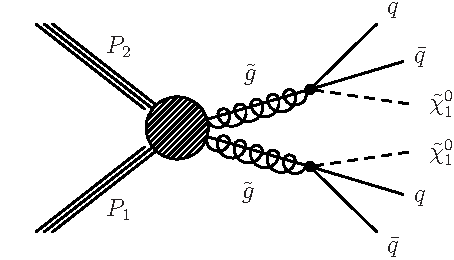
\includegraphics[height=0.15\textwidth]{Supplementary/T1qqqq_feyn_aux}} ~~
   \subfigure[]{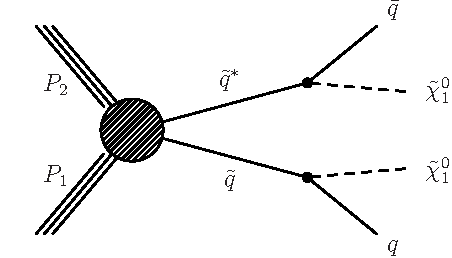
\includegraphics[height=0.15\textwidth]{Supplementary/T2qq_feyn_aux}} \\
   \subfigure[]{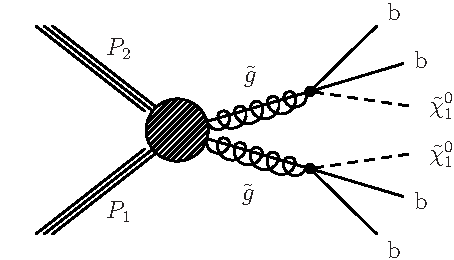
\includegraphics[height=0.15\textwidth]{Supplementary/T1bbbb_feyn_aux}} ~~
   \subfigure[]{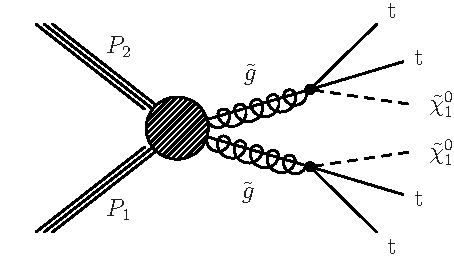
\includegraphics[height=0.15\textwidth]{Supplementary/T1tttt_feyn_aux}} ~~
   \subfigure[]{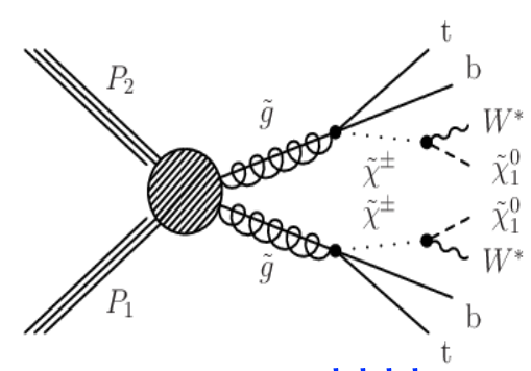
\includegraphics[height=0.15\textwidth]{Supplementary/T1ttbb_feyn_aux}} \\
   \subfigure[]{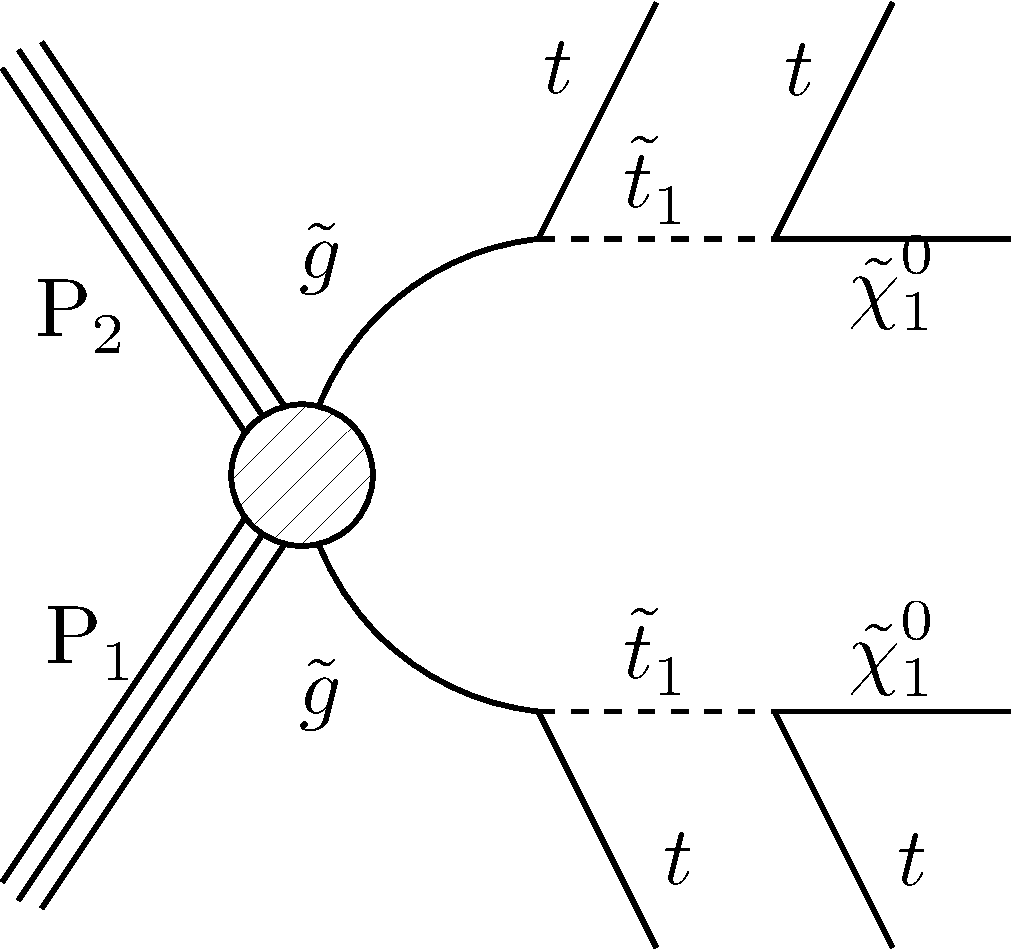
\includegraphics[height=0.15\textwidth]{Supplementary/T5tttt_feyn_aux}} ~~
   \subfigure[]{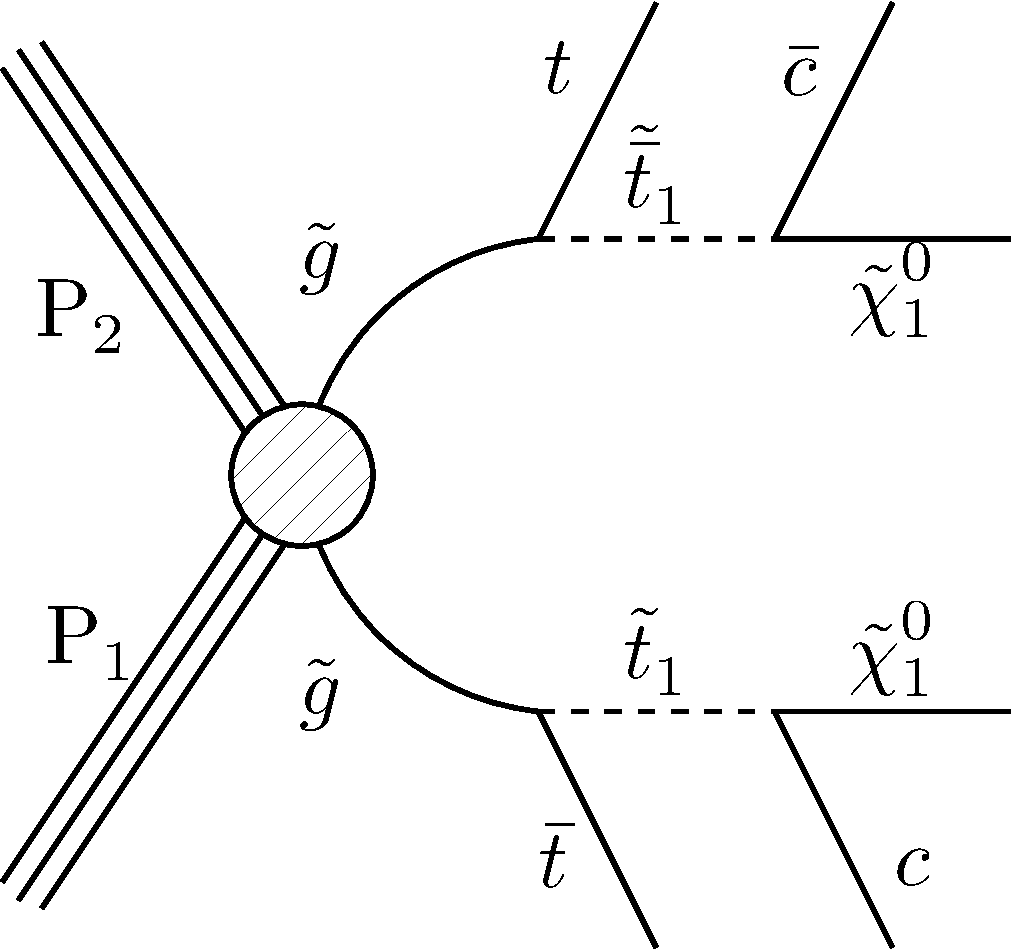
\includegraphics[height=0.15\textwidth]{Supplementary/T5ttcc_feyn_aux}} \\
   \subfigure[]{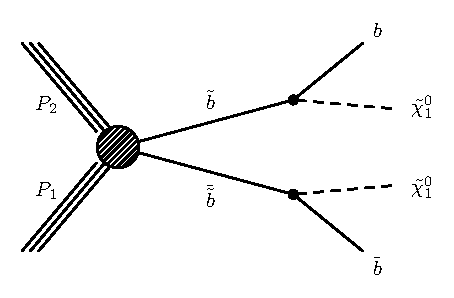
\includegraphics[height=0.15\textwidth]{Supplementary/T2bb_feyn_aux}} ~~
   \subfigure[]{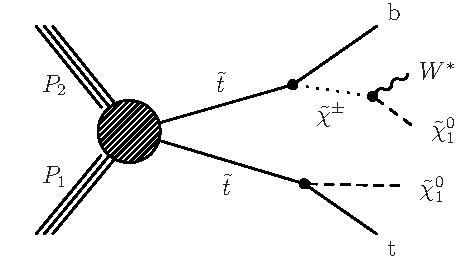
\includegraphics[height=0.15\textwidth]{Supplementary/T2tb_feyn_aux}} ~~
   \subfigure[]{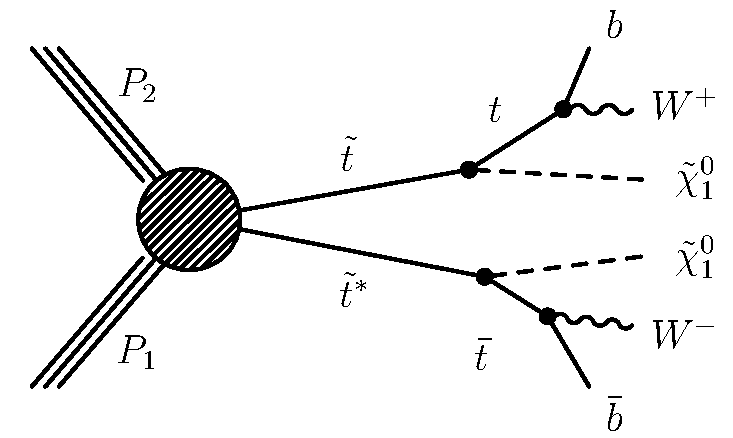
\includegraphics[height=0.15\textwidth]{Supplementary/T2tt_feyn_aux}} \\
   \subfigure[]{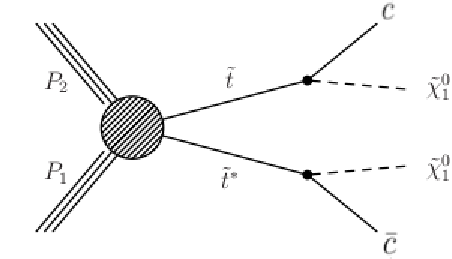
\includegraphics[height=0.15\textwidth]{Supplementary/T2cc_feyn_aux}} ~~
   \subfigure[]{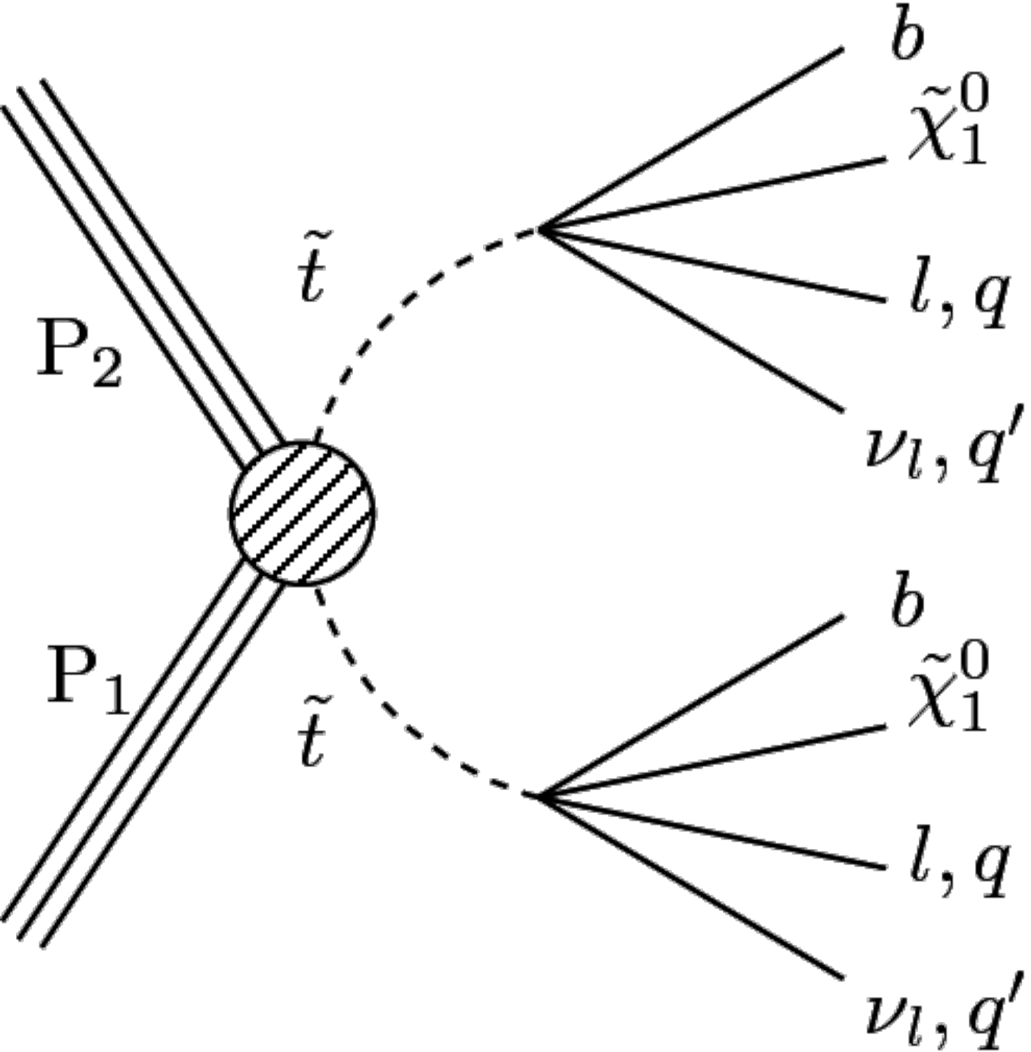
\includegraphics[height=0.15\textwidth]{Supplementary/T2tt_degen_feyn_aux}} ~~
   \subfigure[]{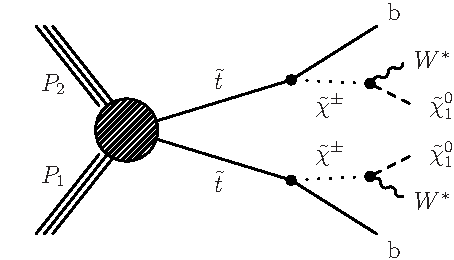
\includegraphics[height=0.15\textwidth]{Supplementary/T2bW_X05_feyn_aux}}
   \caption{ Simplified model diagrams that represent unique
     production and decay modes of supersymmetric particles. The
     figures correspond to the following models: \texttt{T1qqqq} (a),
     \texttt{T2qq} (b), \texttt{T1bbbb} (c), \texttt{T1tttt} (d),
     \texttt{T1ttbb} (e), \texttt{T5tttt\_DM175} (f), \texttt{T5ttcc}
     (g), \texttt{T2bb} (h), \texttt{T2tb} (i), \texttt{T2tt} (j),
     \texttt{T2cc} (k), \texttt{T2tt\_degen} (l), and \texttt{T2bW}
     (m). Three-body decays of gluinos are assumed to proceed through
     off-shell squarks. The diagrams labelled \texttt{T1qqqq} and
     \texttt{T2qq} depict, respectively, the gluino-mediated and
     direct production of light-flavour squarks. The diagrams labelled
     \texttt{T1bbbb}, \texttt{T1tttt}, and \texttt{T1ttbb} depict
     models involving the gluino-mediated production of off-shell
     third-generation squarks. The diagrams labelled
     \texttt{T5tttt\_DM175} and \texttt{T5ttcc} depict ``natural''
     models comprising gluino-mediated production of on-shell top
     squarks. Finally, the remaining six diagrams depict the direct
     production of third-generation squarks, decaying via a range of
     channels.  }
   \label{fig:simplified-models}
 \end{center}
\end{figure*}


\clearpage
\begin{figure*}[!h]
  \begin{center}
    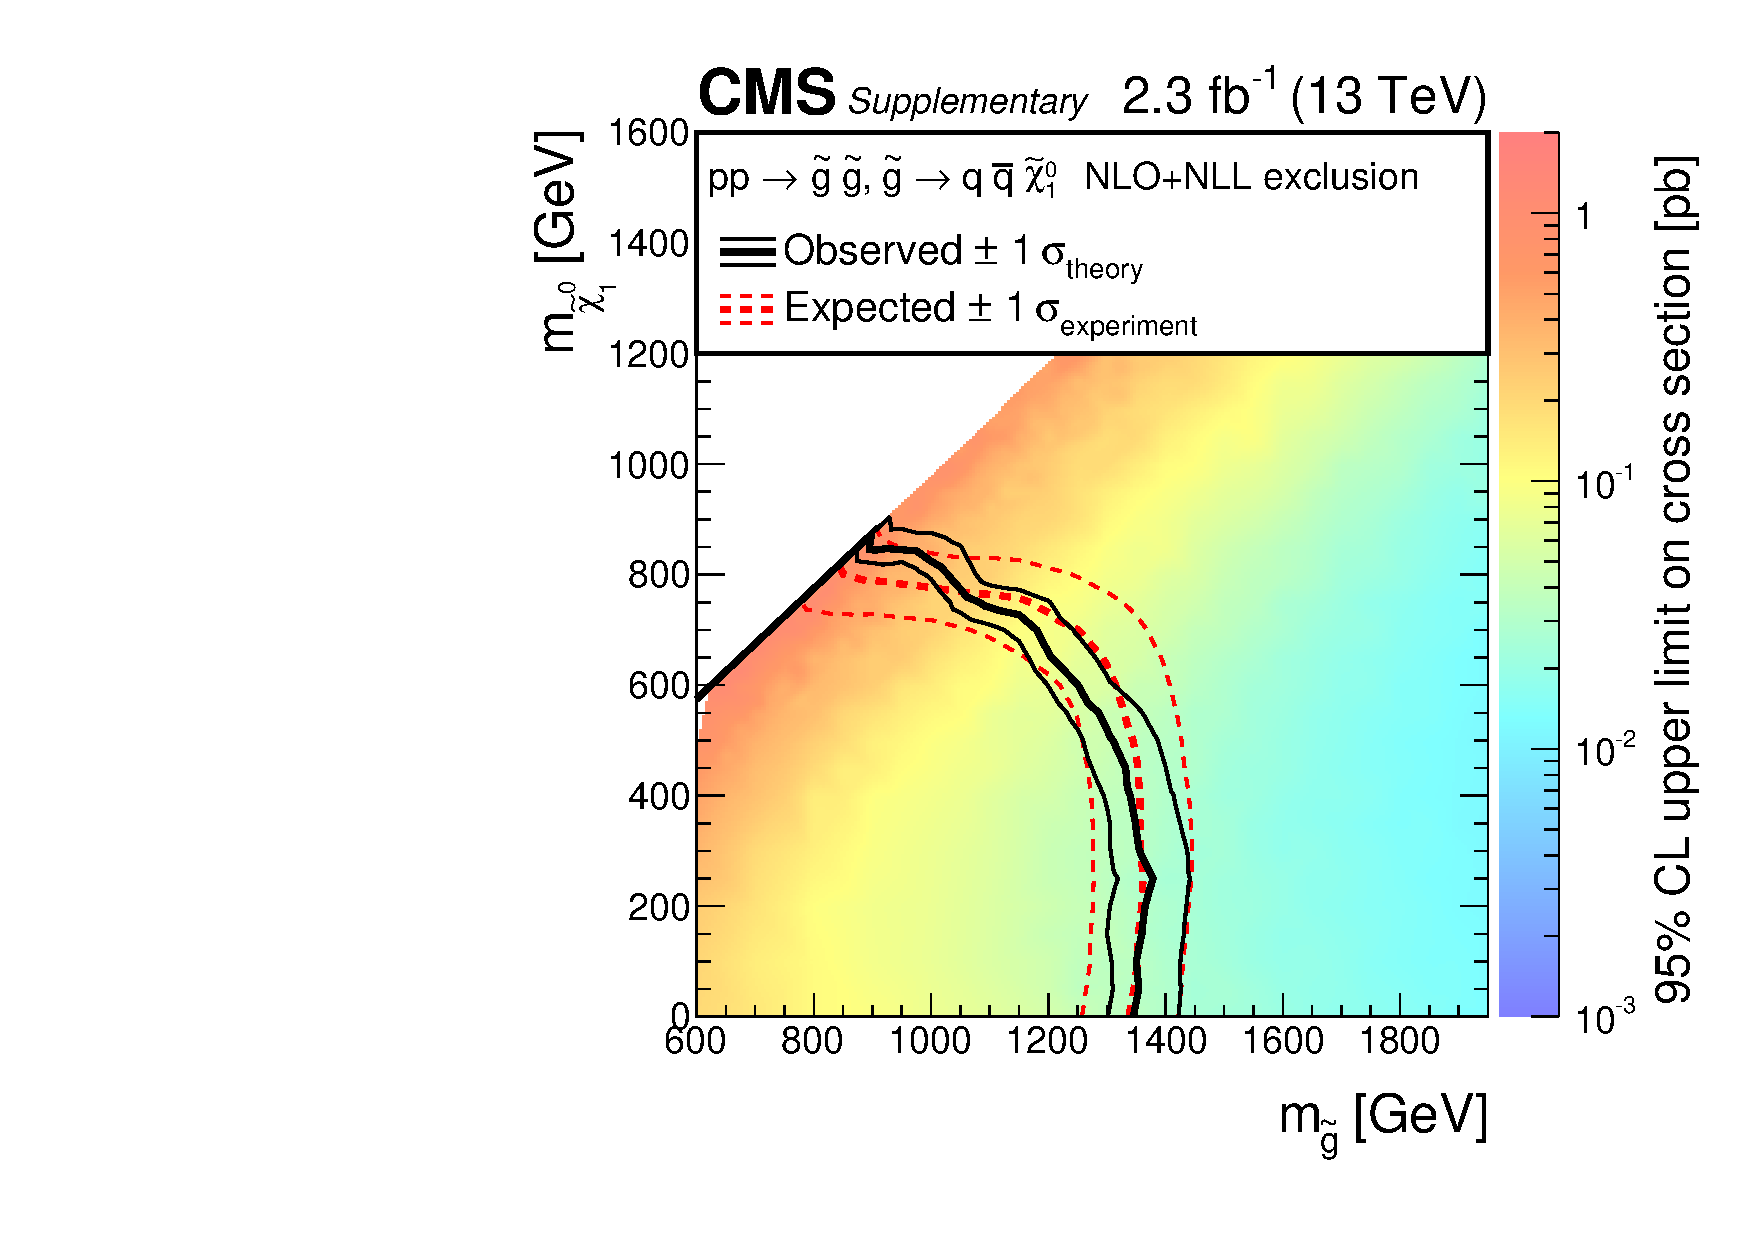
\includegraphics[width=0.49\textwidth]{Supplementary/RA1T1qqqqXSEC_aux} \, 
    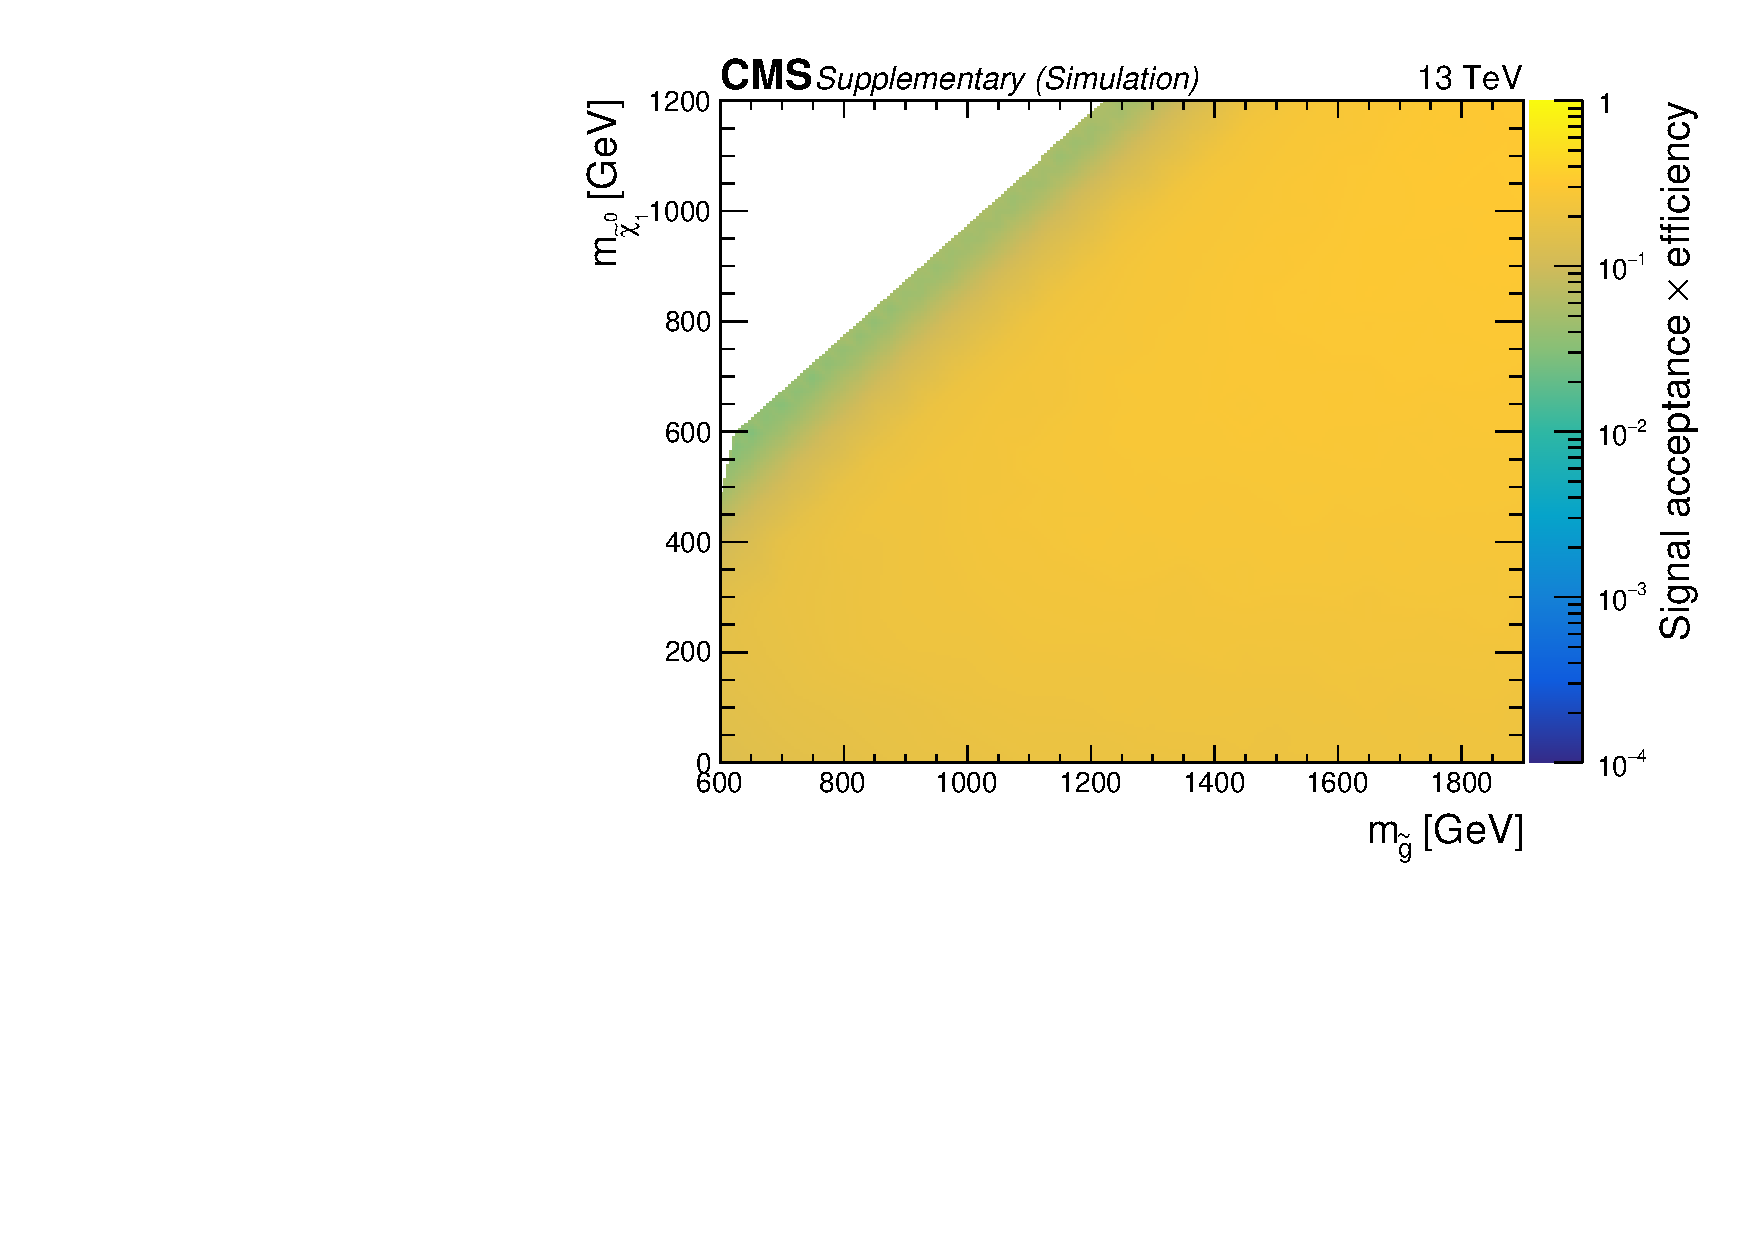
\includegraphics[width=0.49\textwidth]{Supplementary/T1qqqq_eff} \,     
  \end{center}
  \caption{Left: (coloured histogram) upper limit on the cross section in the $(m_{\,\PSg}, m_{\PSGczDo})$ plane for the \texttt{T1qqqq} model. 
  The black (red) solid line is the observed (expected) exclusion. The red dashed lines are the $\pm1\sigma$ expected exclusion due to experimental uncertainties. 
  The $\pm1\sigma$ observed exclusion due to theoretical uncertainties on the signal cross section are shown as thin black lines. 
  Right: signal efficiency for the search regions included in the limit calculation as a function $(m_{\,\PSg}, m_{\PSGczDo})$ plane for the \texttt{T1qqqq} model. 
  \label{fig:T1qqqq_excl}}
\end{figure*}

\clearpage
\begin{figure*}[!h]
  \begin{center}
    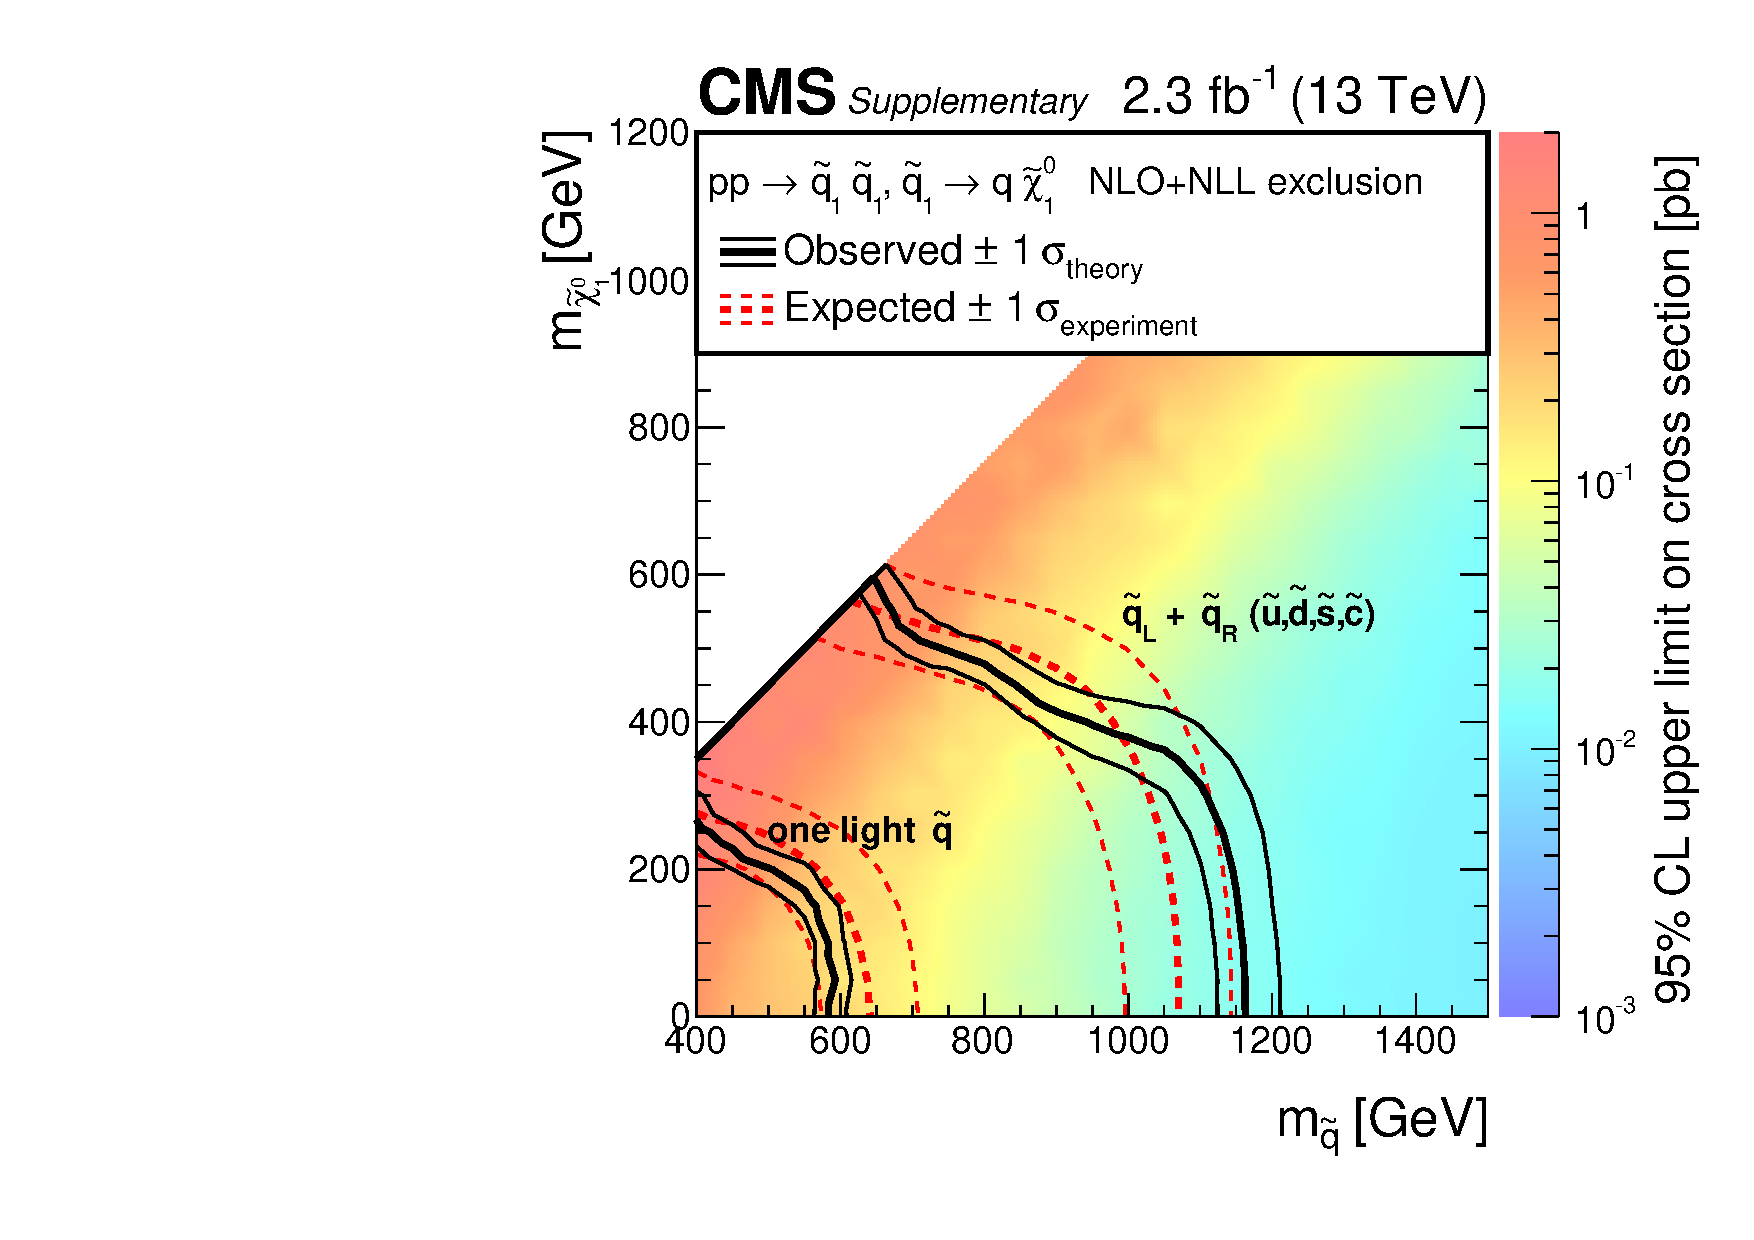
\includegraphics[width=0.49\textwidth]{Supplementary/RA1T2qqXSEC_aux} \, 
    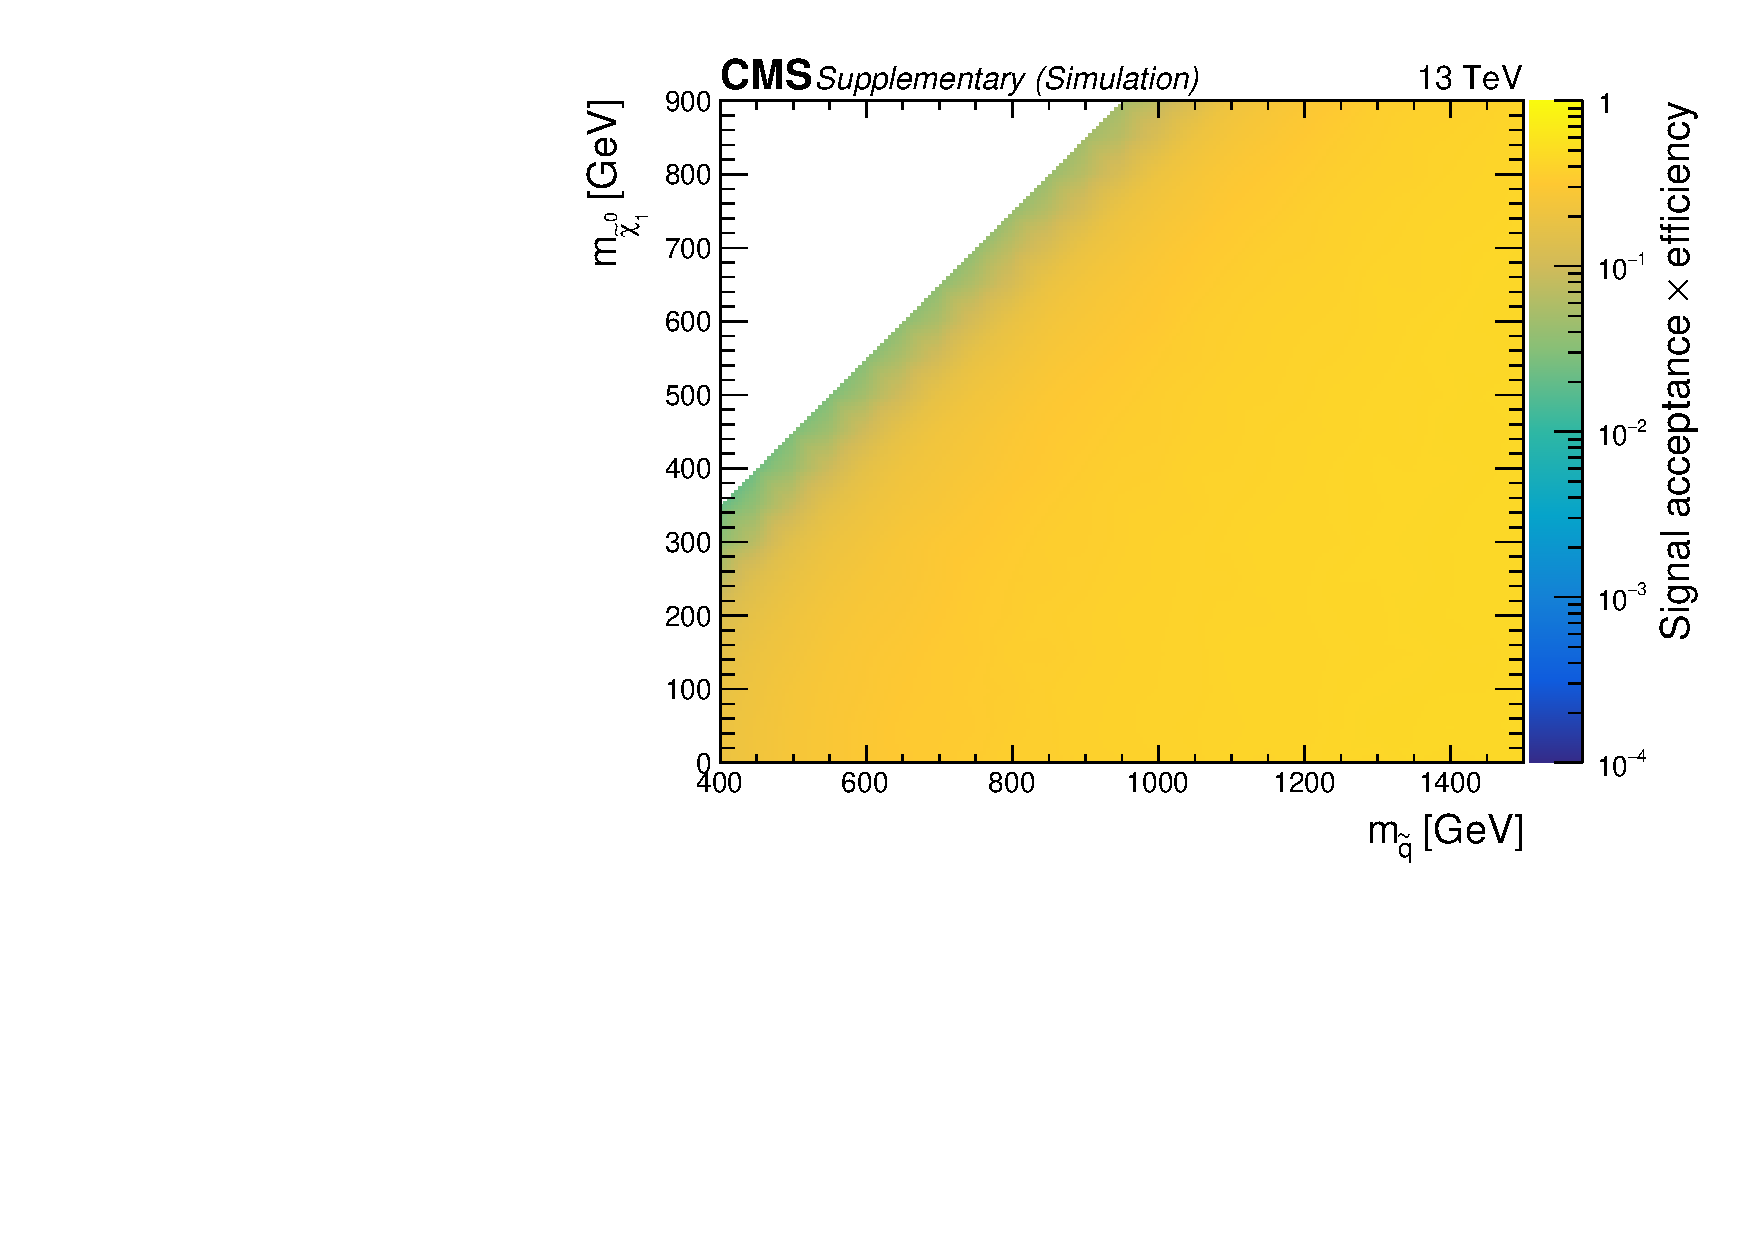
\includegraphics[width=0.49\textwidth]{Supplementary/T2qq_eff} \,     
  \end{center}
  \caption{Left: (coloured histogram) upper limit on the cross section in the $(m_{\,\PSQ}, m_{\PSGczDo})$ plane for the \texttt{T2qq} model. 
  The black (red) solid line is the observed (expected) exclusion. The red dashed lines are the $\pm1\sigma$ expected exclusion due to experimental uncertainties. 
  The $\pm1\sigma$ observed exclusion due to theoretical uncertainties on the signal cross section are shown as thin black lines. 
  Right: signal efficiency for the search regions included in the limit calculation as a function $(m_{\,\PSQ}, m_{\PSGczDo})$ plane for the \texttt{T2qq} model. 
  \label{fig:T2qq_excl}}
\end{figure*}


\clearpage
\begin{figure*}[!h]
  \begin{center}
    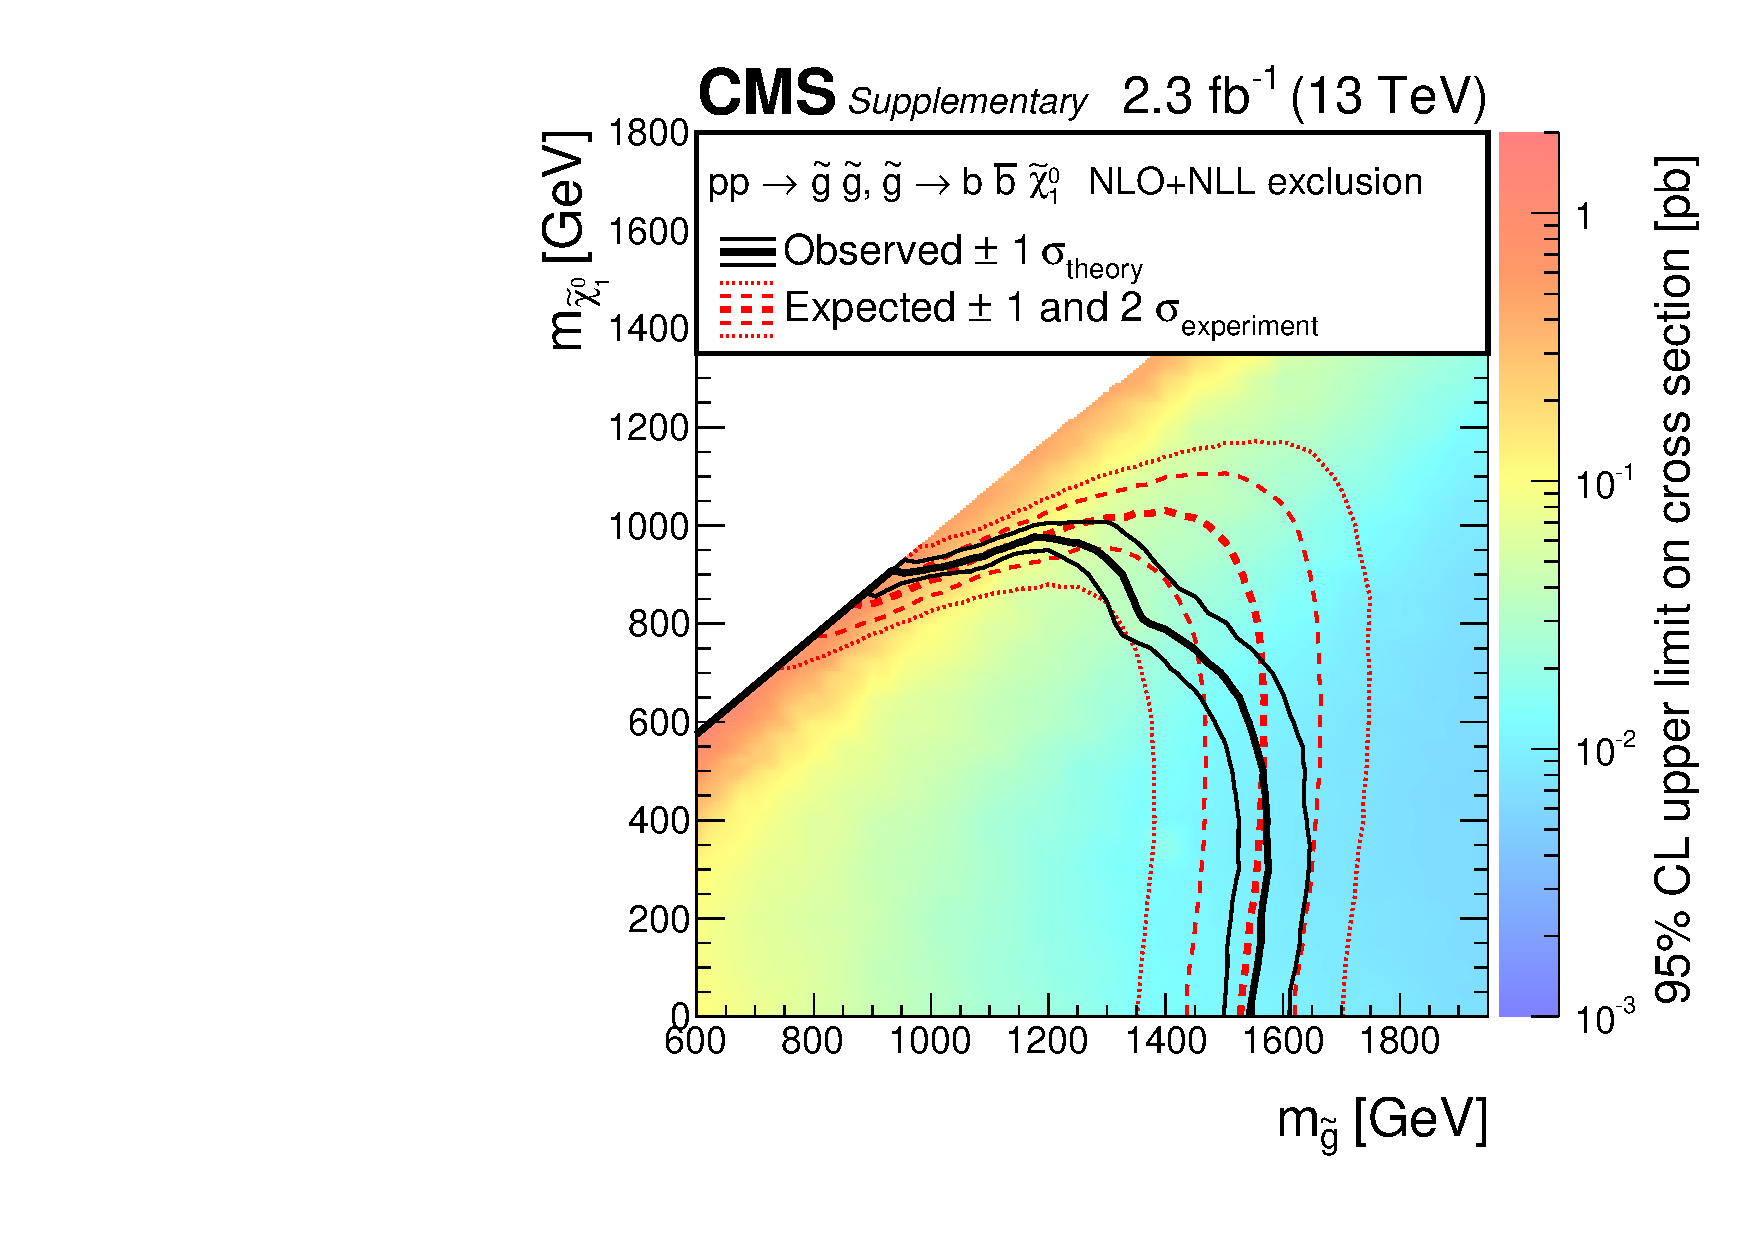
\includegraphics[width=0.49\textwidth]{Supplementary/RA1T1bbbbXSEC_aux} \, 
    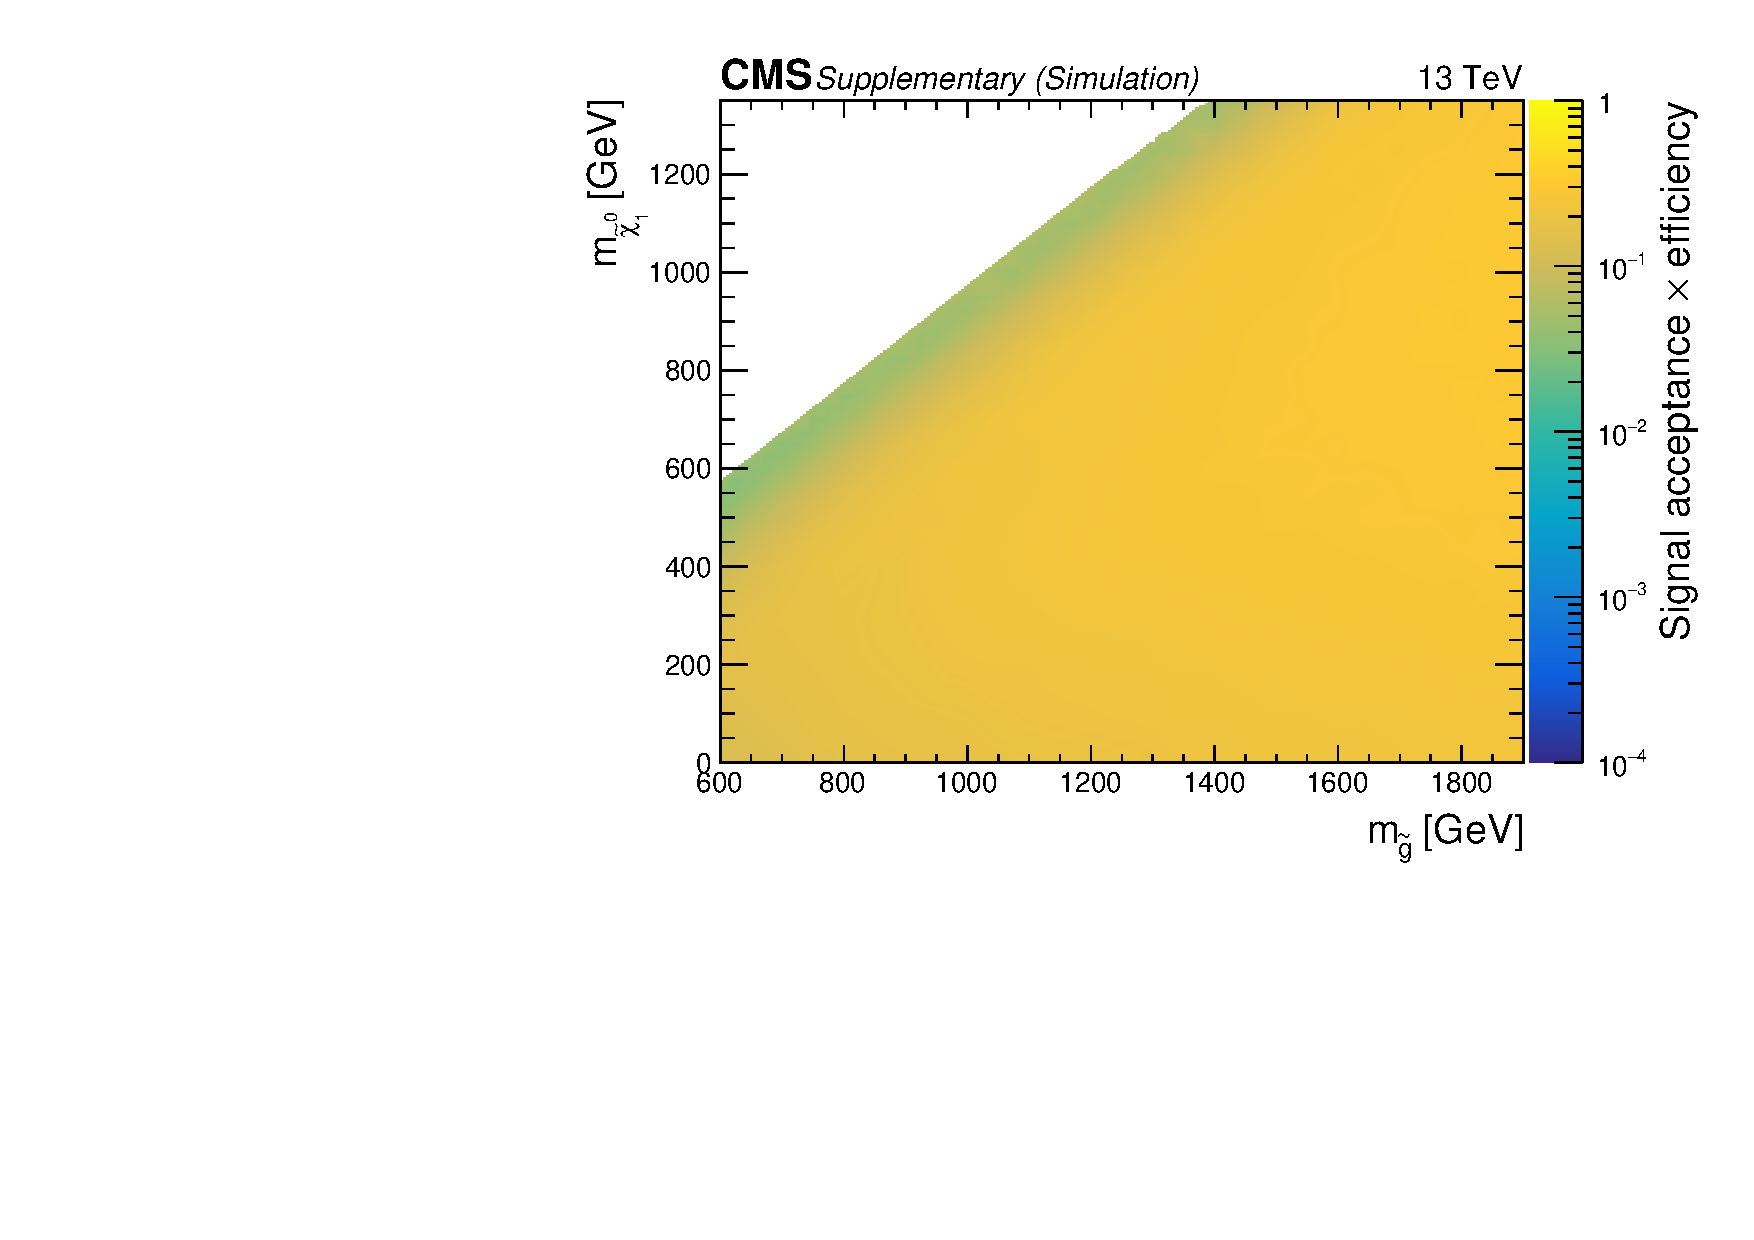
\includegraphics[width=0.49\textwidth]{Supplementary/T1bbbb_eff} \,     
  \end{center}
  \caption{Left: (coloured histogram) upper limit on the cross section in the $(m_{\,\PSg}, m_{\PSGczDo})$ plane for the \texttt{T1bbbb} model. 
  The black (red) solid line is the observed (expected) exclusion. The red dashed lines are the $\pm1\sigma$ expected exclusion due to experimental uncertainties. 
  The $\pm1\sigma$ observed exclusion due to theoretical uncertainties on the signal cross section are shown as thin black lines. 
  Right: signal efficiency for the search regions included in the limit calculation as a function $(m_{\,\PSg}, m_{\PSGczDo})$ plane for the \texttt{T1bbbb} model. 
  \label{fig:T1bbbb_excl}}
\end{figure*}

\clearpage
\begin{figure*}[!h]
  \begin{center}
    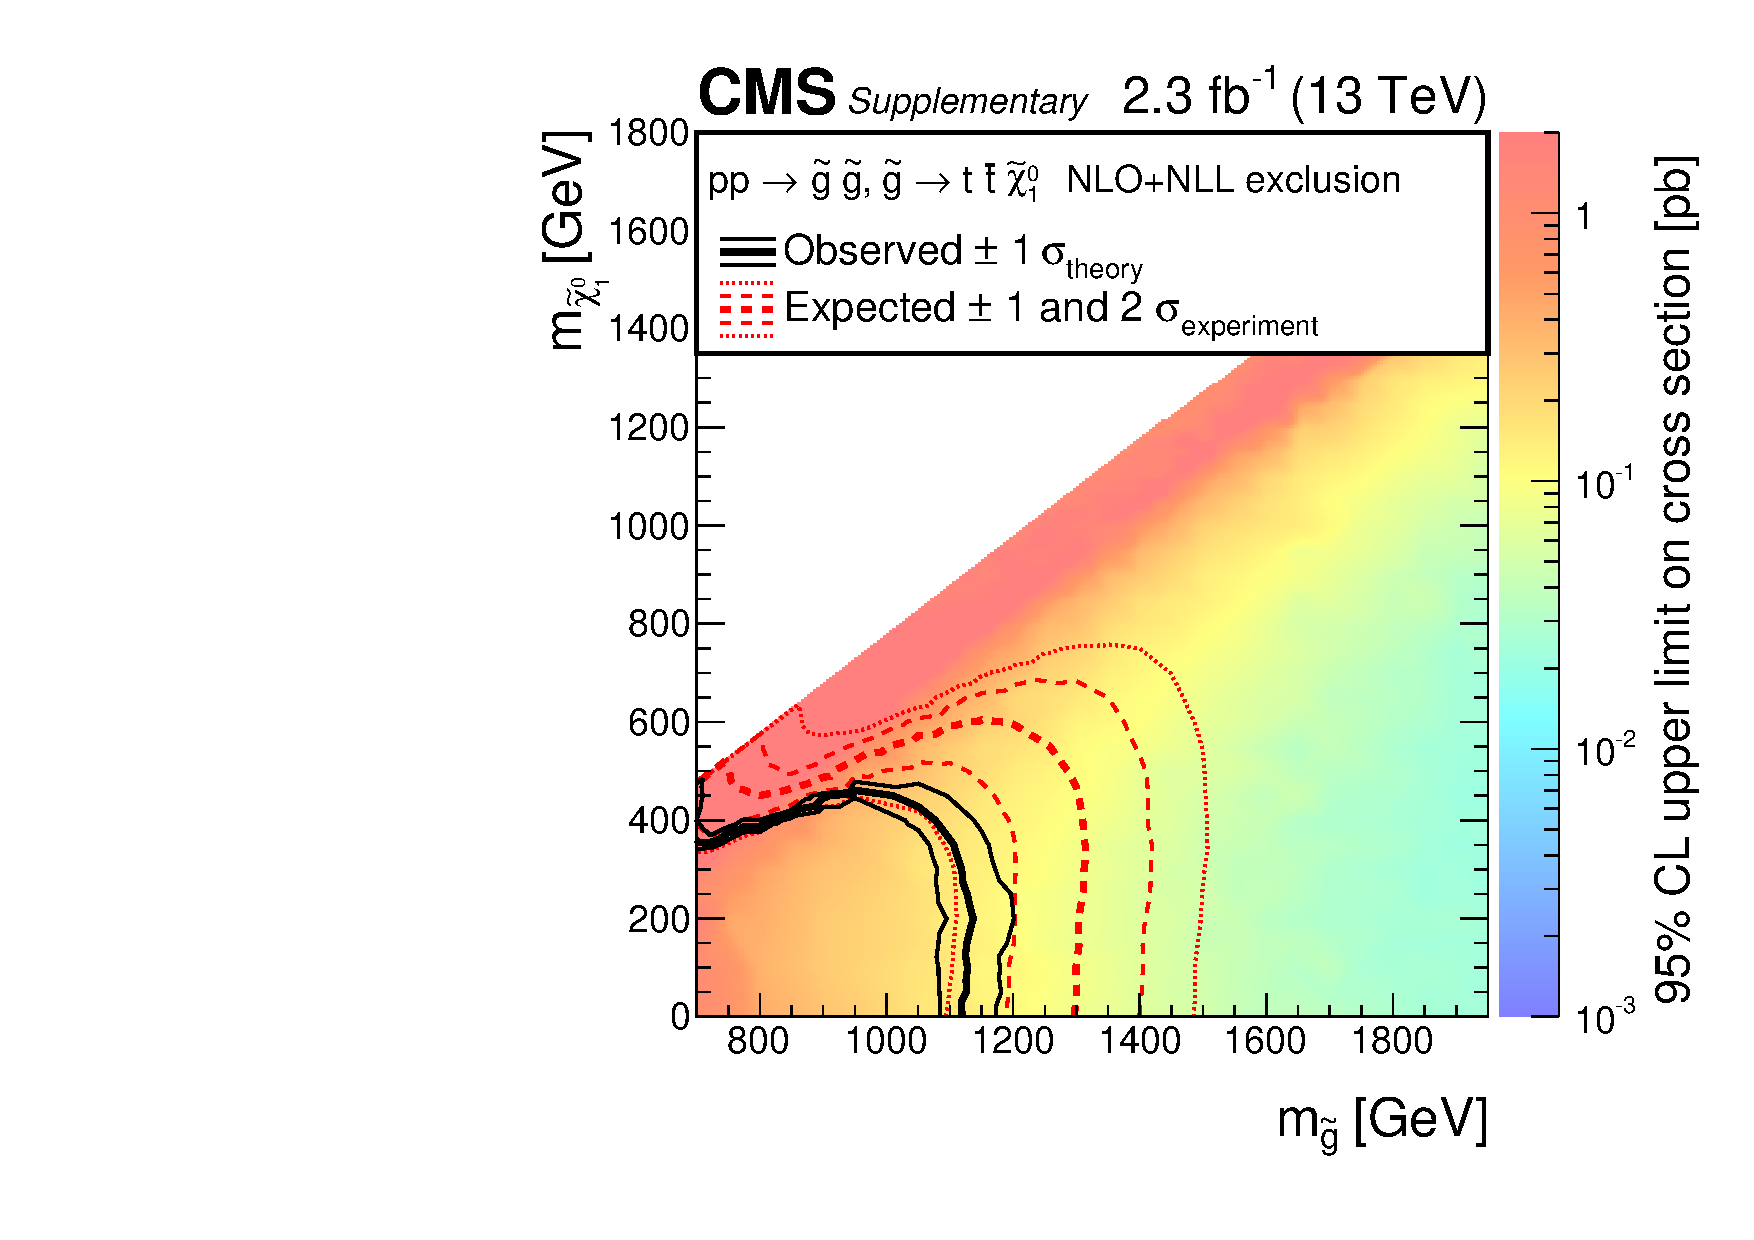
\includegraphics[width=0.49\textwidth]{Supplementary/RA1T1ttttXSEC_aux} \, 
    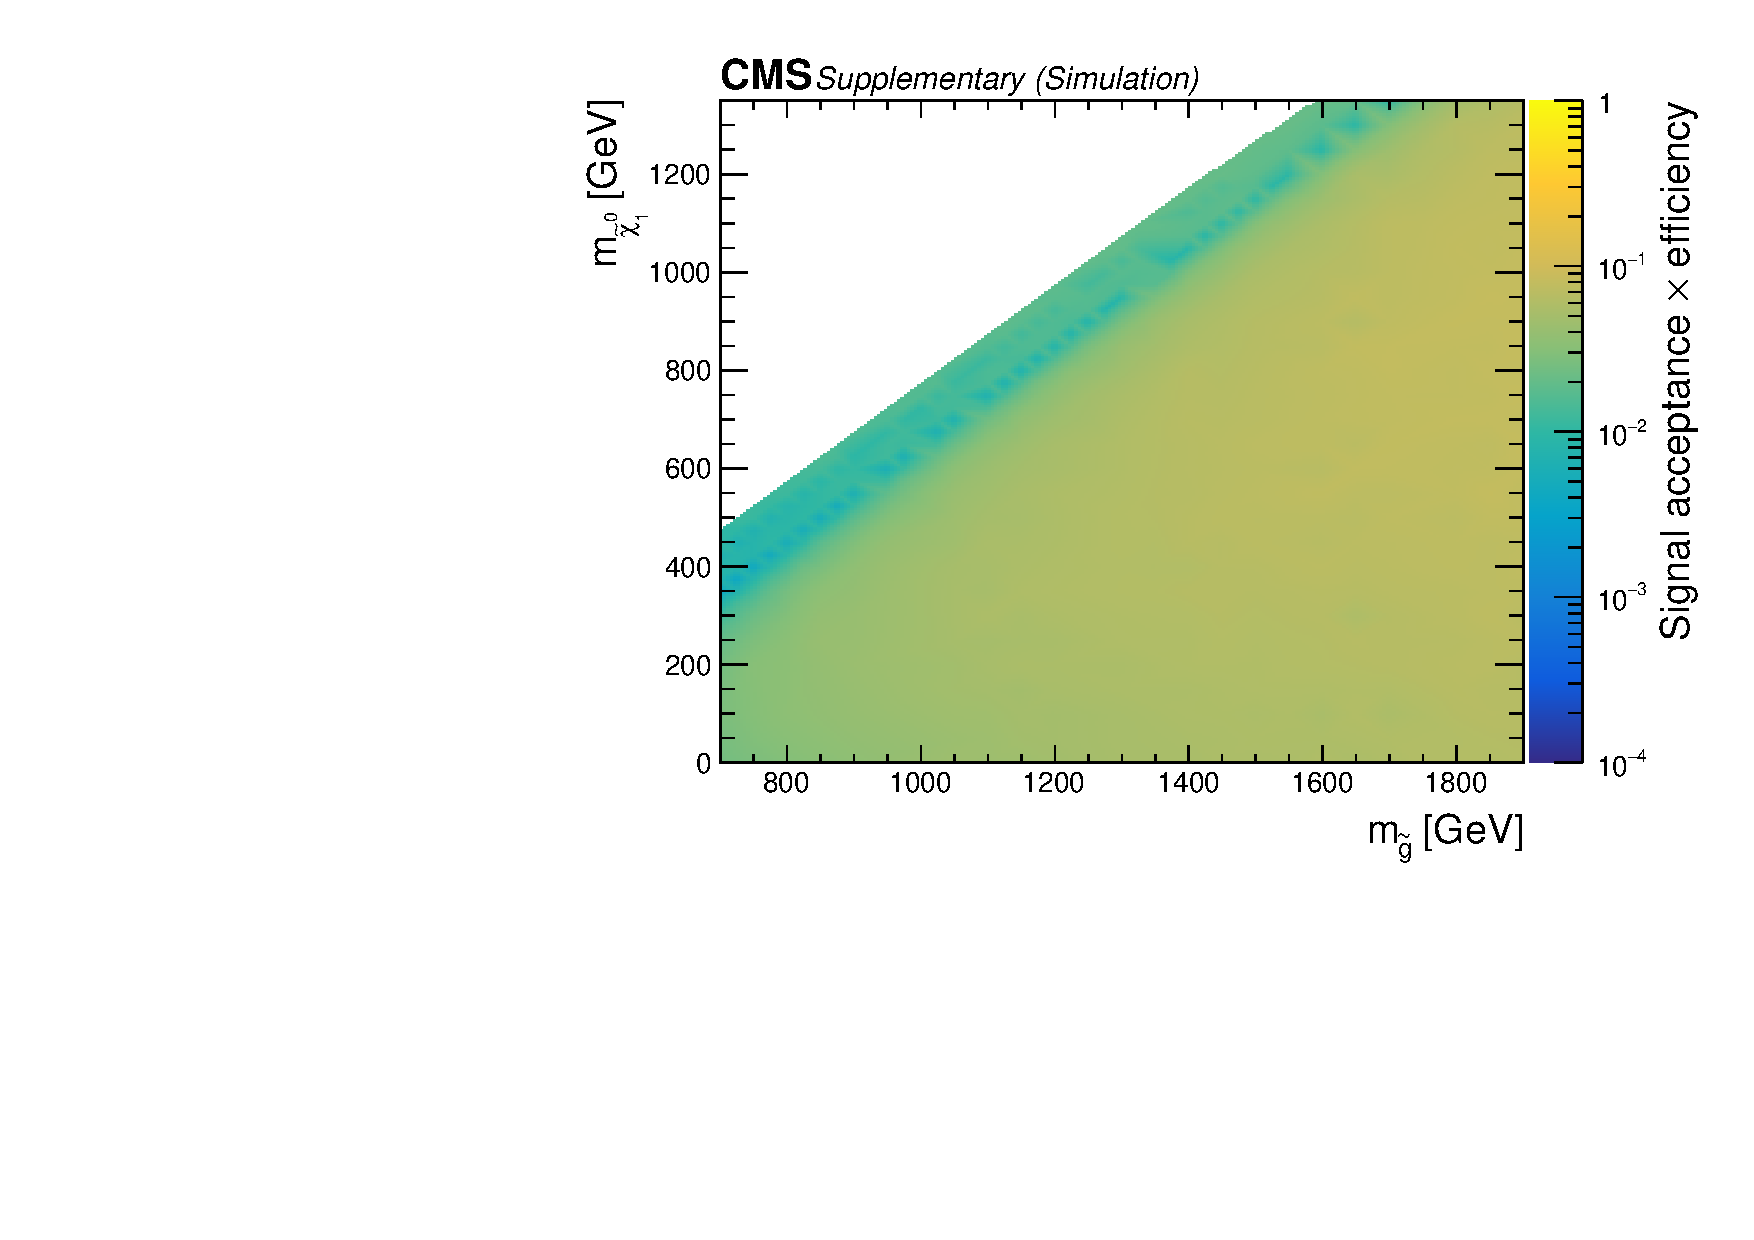
\includegraphics[width=0.49\textwidth]{Supplementary/T1tttt_eff} \,     
  \end{center}
  \caption{Left: (coloured histogram) upper limit on the cross section in the $(m_{\,\PSg}, m_{\PSGczDo})$ plane for the \texttt{T1tttt} model. 
  The black (red) solid line is the observed (expected) exclusion. The red dashed lines are the $\pm1\sigma$ expected exclusion due to experimental uncertainties. 
  The $\pm1\sigma$ observed exclusion due to theoretical uncertainties on the signal cross section are shown as thin black lines. 
  Right: signal efficiency for the search regions included in the limit calculation as a function $(m_{\,\PSg}, m_{\PSGczDo})$ plane for the \texttt{T1tttt} model. 
  \label{fig:T1tttt_excl}}
\end{figure*}

\clearpage
\begin{figure*}[!h]
  \begin{center}
    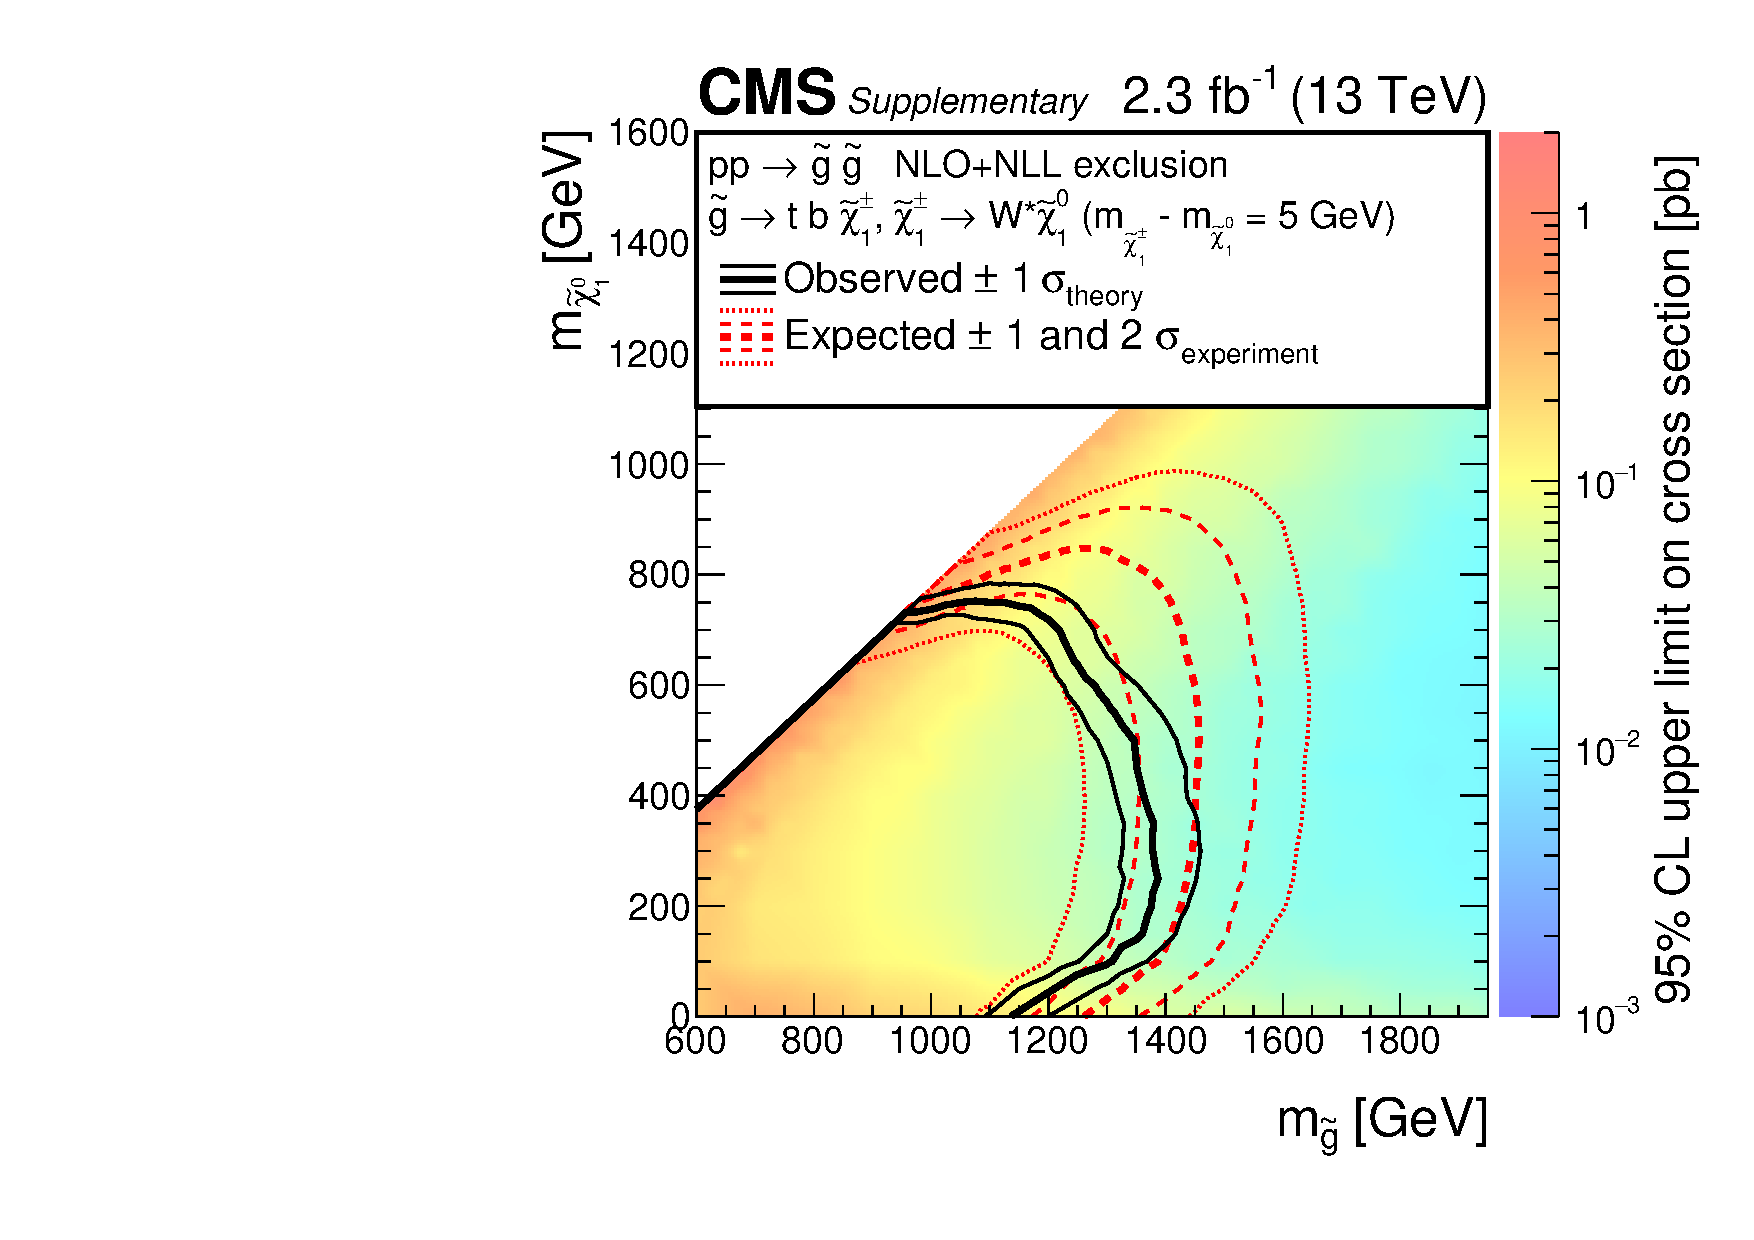
\includegraphics[width=0.49\textwidth]{Supplementary/RA1T1ttbbXSEC_aux} \, 
    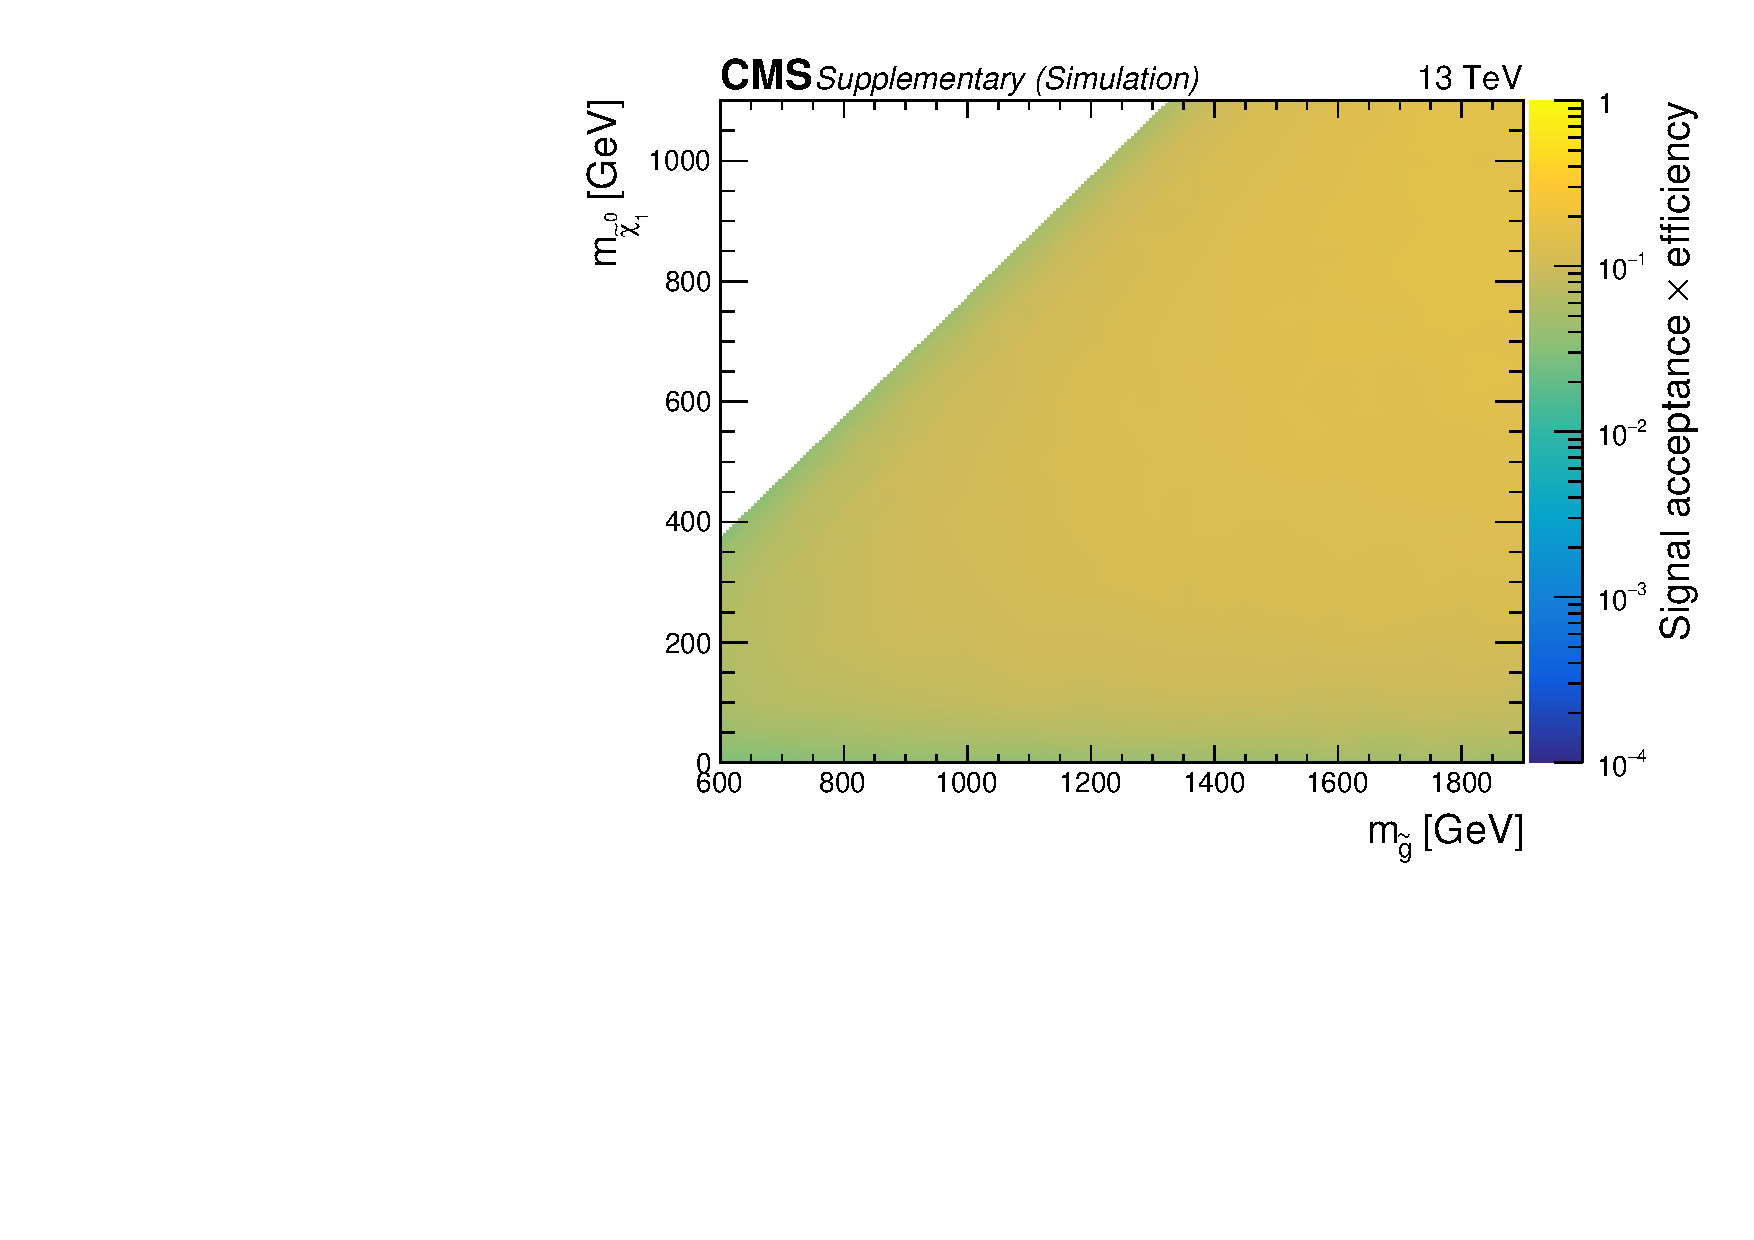
\includegraphics[width=0.49\textwidth]{Supplementary/T1ttbb_eff} \,     
  \end{center}
  \caption{Left: (coloured histogram) upper limit on the cross section in the $(m_{\,\PSg}, m_{\PSGczDo})$ plane for the \texttt{T1ttbb} model. 
  The black (red) solid line is the observed (expected) exclusion. The red dashed lines are the $\pm1\sigma$ expected exclusion due to experimental uncertainties. 
  The $\pm1\sigma$ observed exclusion due to theoretical uncertainties on the signal cross section are shown as thin black lines. 
  Right: signal efficiency for the search regions included in the limit calculation as a function $(m_{\,\PSg}, m_{\PSGczDo})$ plane for the \texttt{T1ttbb} model. 
  \label{fig:T1ttbb_excl}}
\end{figure*}

\clearpage
\begin{figure*}[!h]
  \begin{center}
    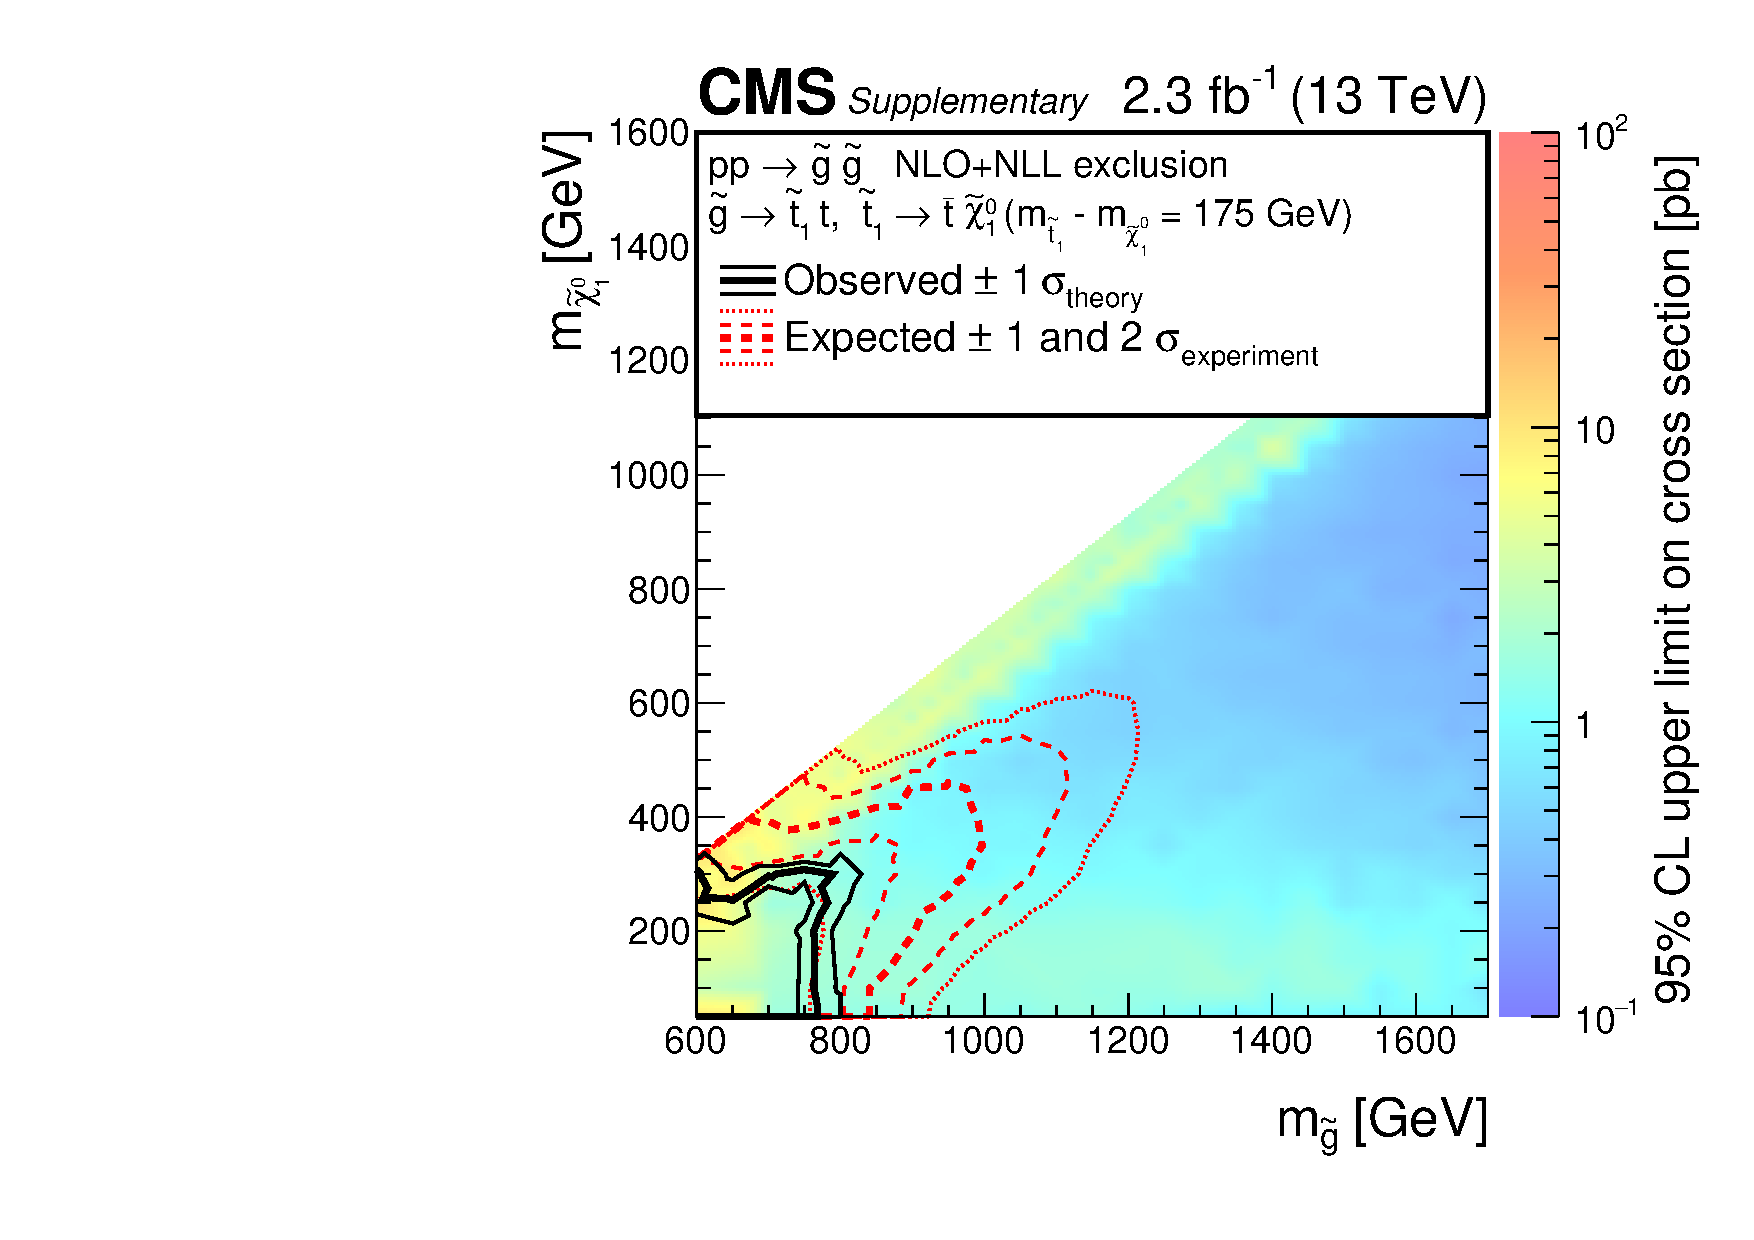
\includegraphics[width=0.49\textwidth]{Supplementary/RA1T5ttttDM175XSEC_aux} \, 
    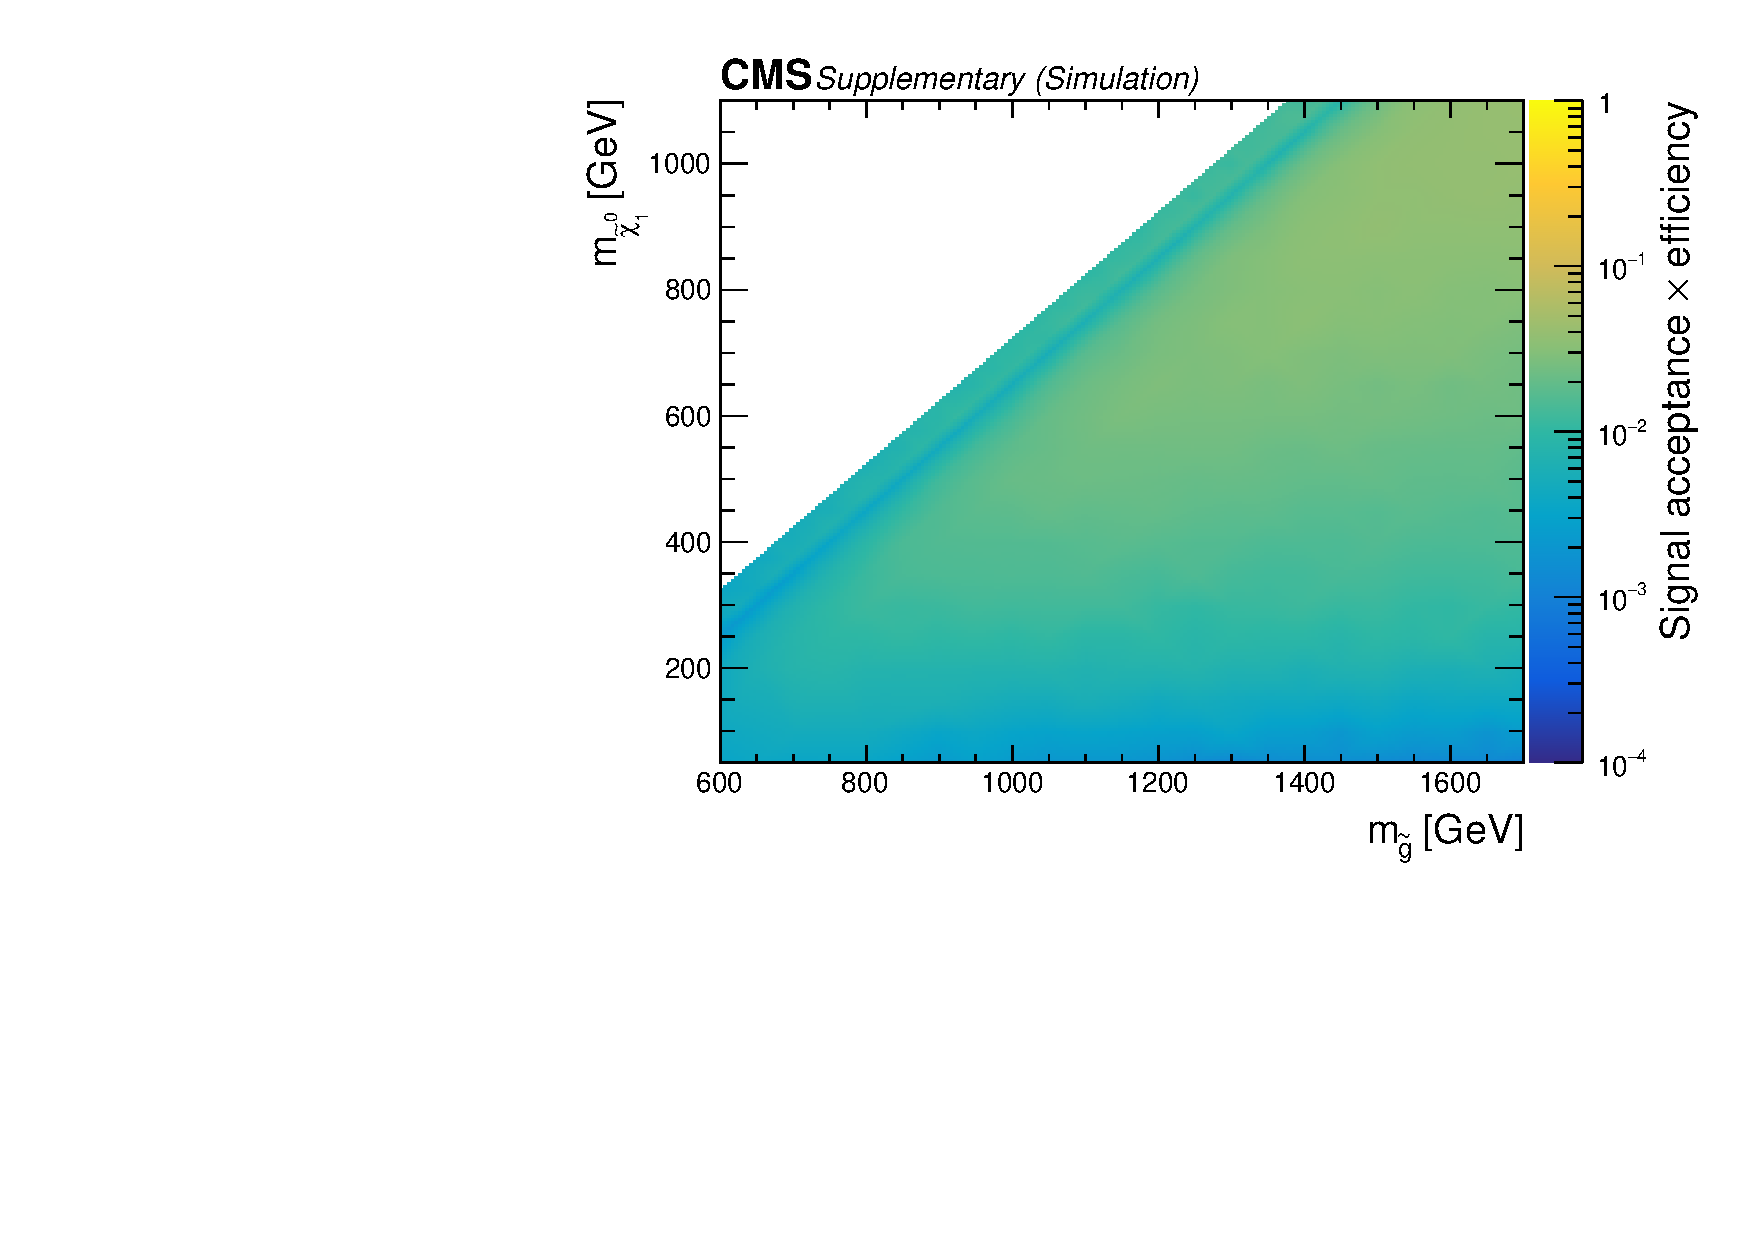
\includegraphics[width=0.49\textwidth]{Supplementary/T5ttttDM175_eff} \,     
  \end{center}
  \caption{Left: (coloured histogram) upper limit on the cross section in the $(m_{\,\PSg}, m_{\PSGczDo})$ plane for the \texttt{T5tttt\_DM175} model. 
  The black (red) solid line is the observed (expected) exclusion. The red dashed lines are the $\pm1\sigma$ expected exclusion due to experimental uncertainties. 
  The $\pm1\sigma$ observed exclusion due to theoretical uncertainties on the signal cross section are shown as thin black lines. 
  Right: signal efficiency for the search regions included in the limit calculation as a function $(m_{\,\PSg}, m_{\PSGczDo})$ plane for the \texttt{T5tttt\_DM175} model. 
  \label{fig:T5ttttDM175_excl}}
\end{figure*}

\clearpage
\begin{figure*}[!h]
  \begin{center}
    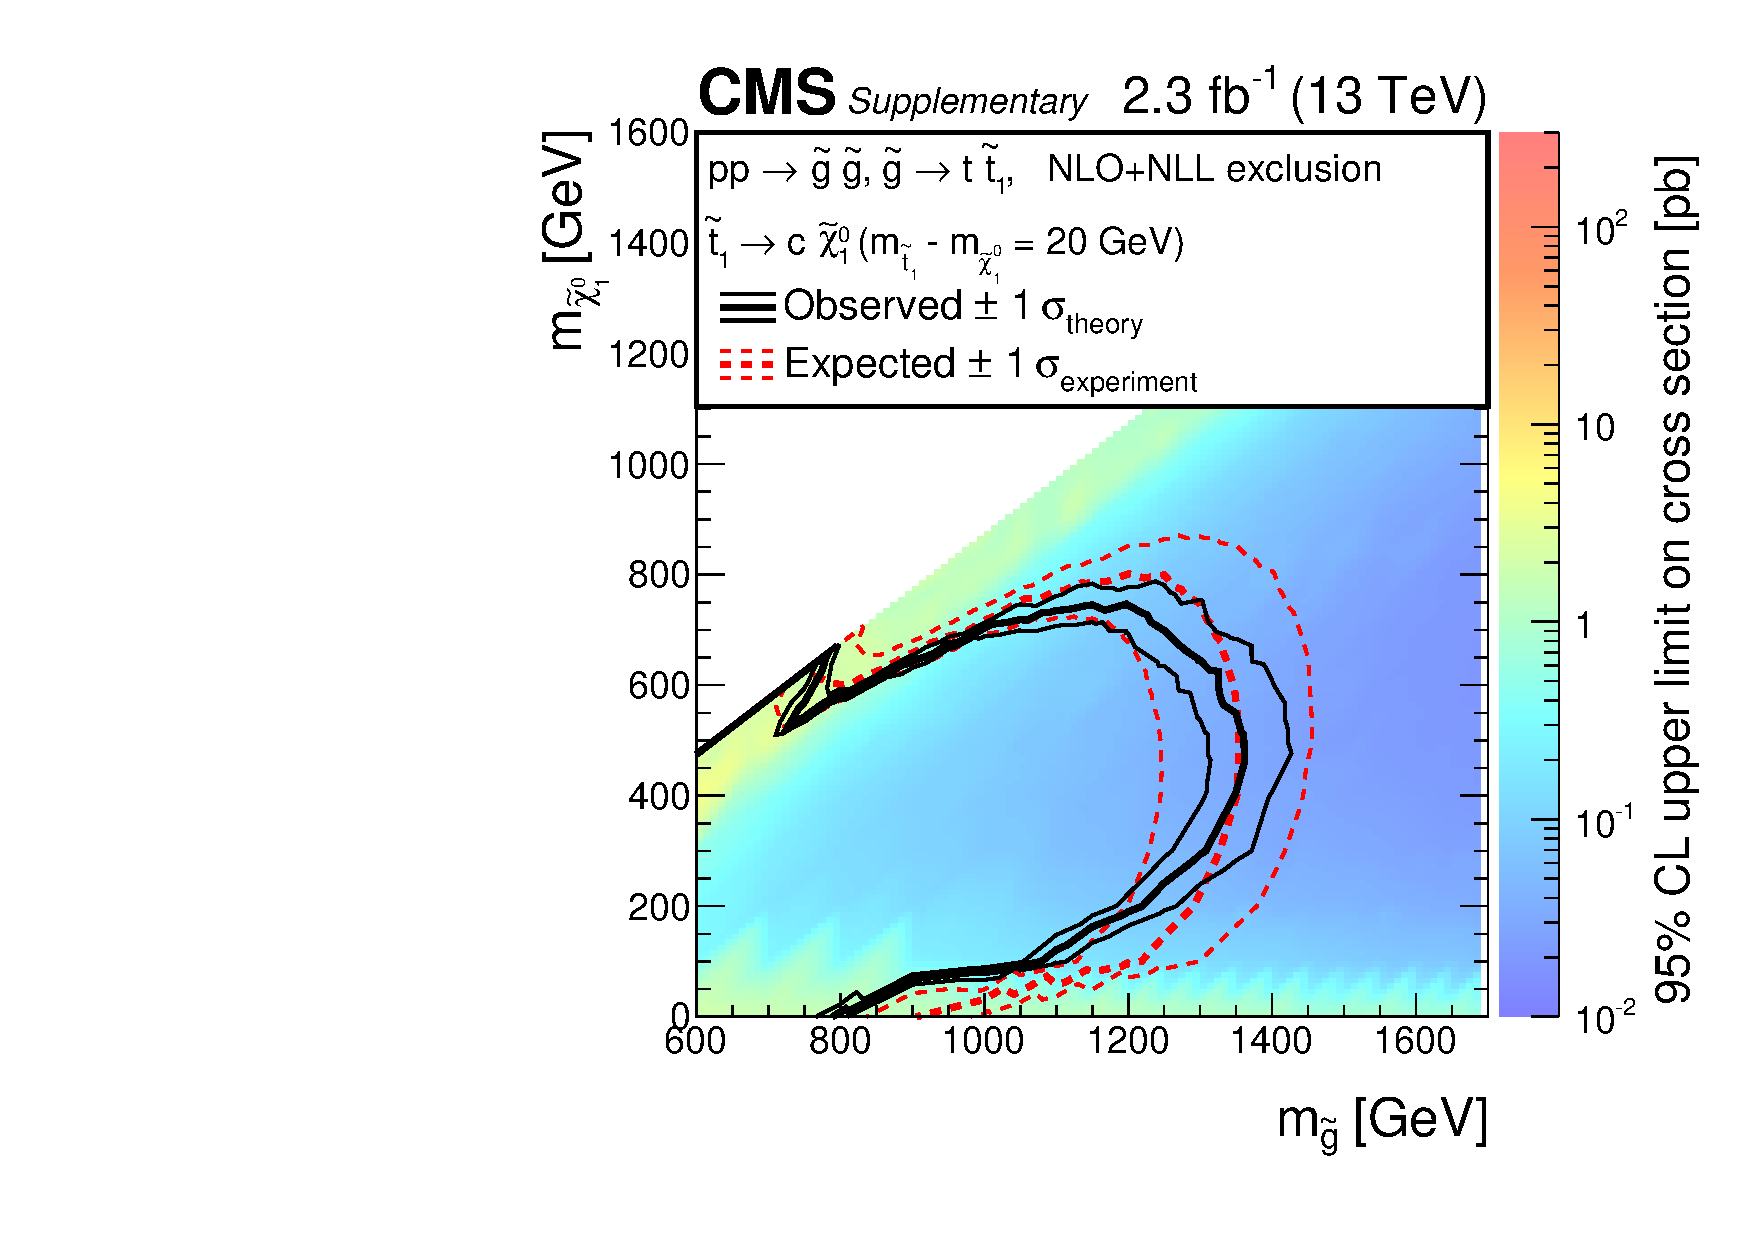
\includegraphics[width=0.49\textwidth]{Supplementary/RA1T5ttccXSEC_aux} \, 
    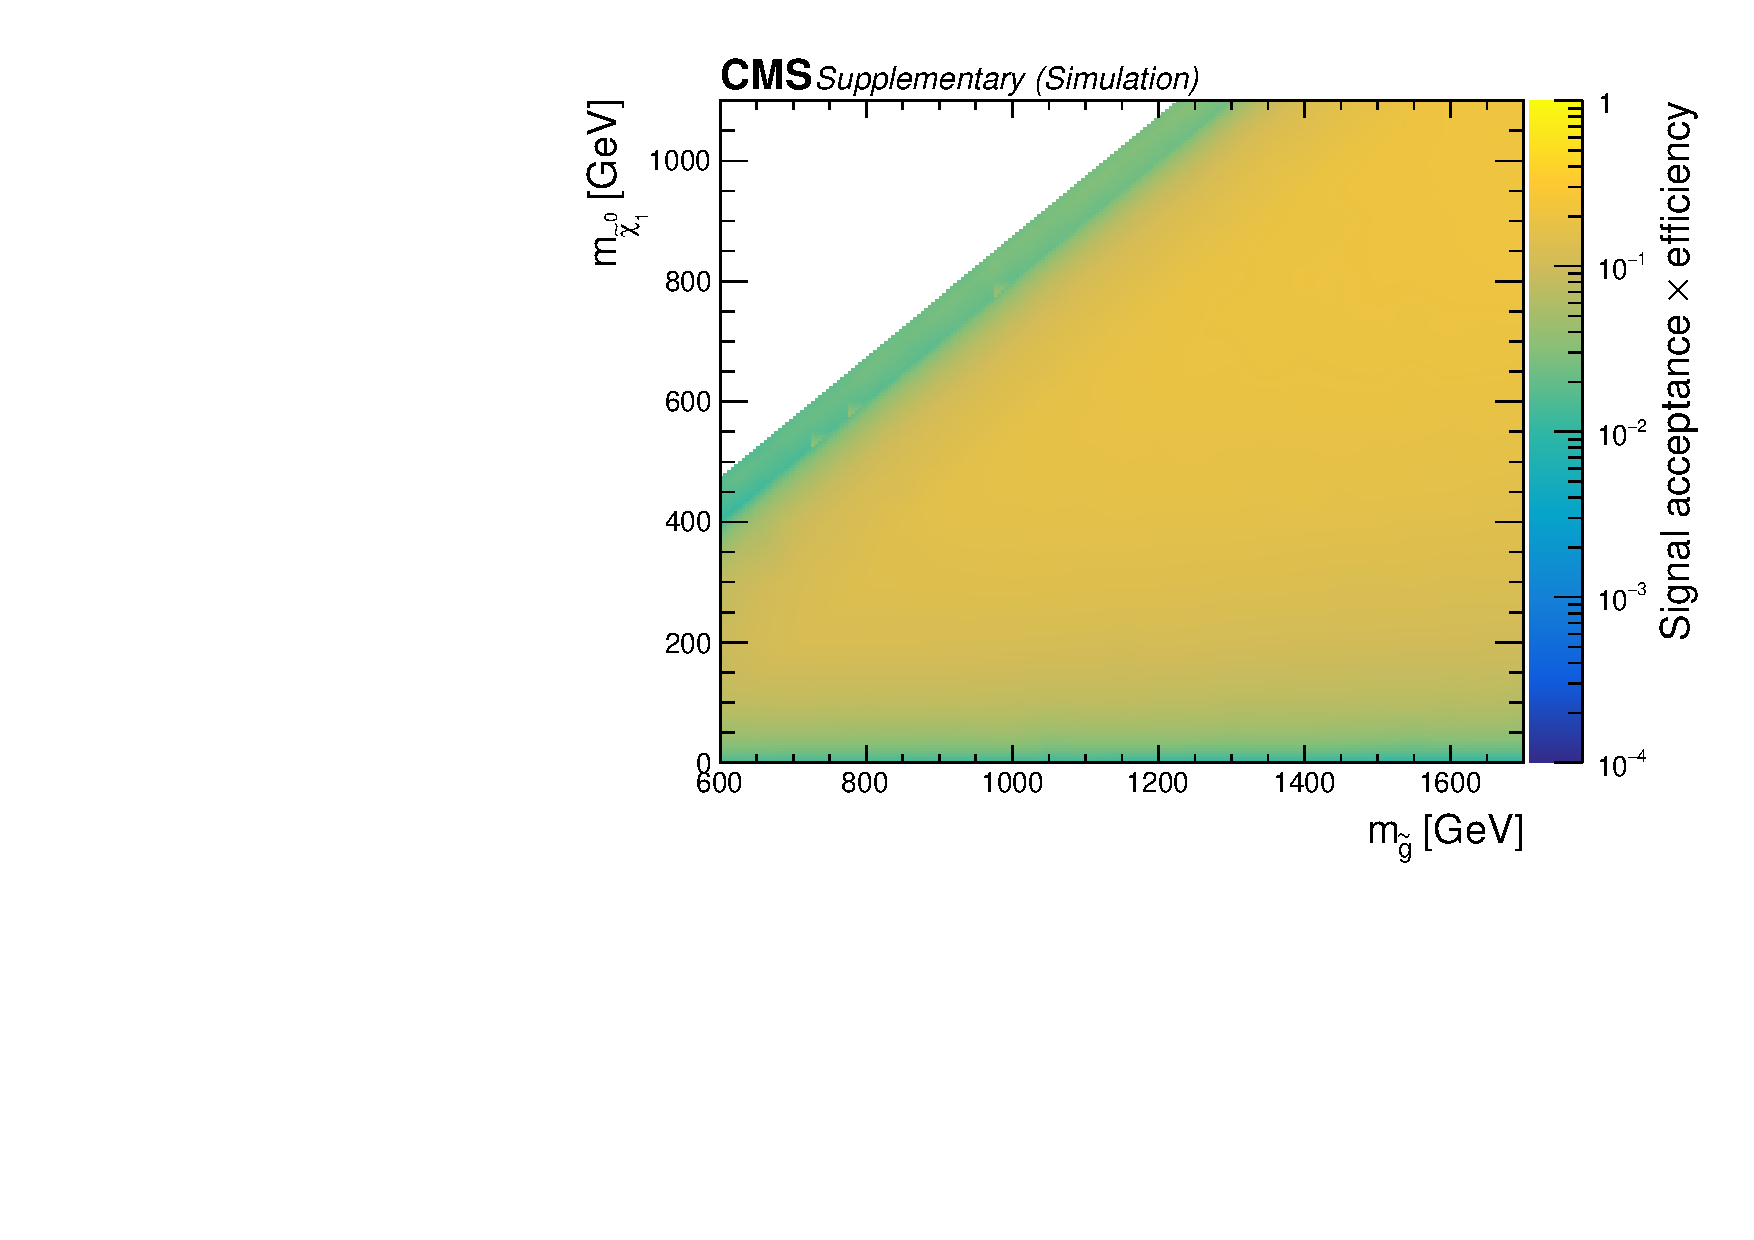
\includegraphics[width=0.49\textwidth]{Supplementary/T5ttcc_eff} \,     
  \end{center}
  \caption{Left: (coloured histogram) upper limit on the cross section in the $(m_{\,\PSg}, m_{\PSGczDo})$ plane for the \texttt{T5ttcc} model. 
  The black (red) solid line is the observed (expected) exclusion. The red dashed lines are the $\pm1\sigma$ expected exclusion due to experimental uncertainties. 
  The $\pm1\sigma$ observed exclusion due to theoretical uncertainties on the signal cross section are shown as thin black lines. 
  Right: signal efficiency for the search regions included in the limit calculation as a function $(m_{\,\PSg}, m_{\PSGczDo})$ plane for the \texttt{T5ttcc} model. 
  \label{fig:T5ttcc_excl}}
\end{figure*}


\clearpage
\begin{figure*}[!h]
  \begin{center}
    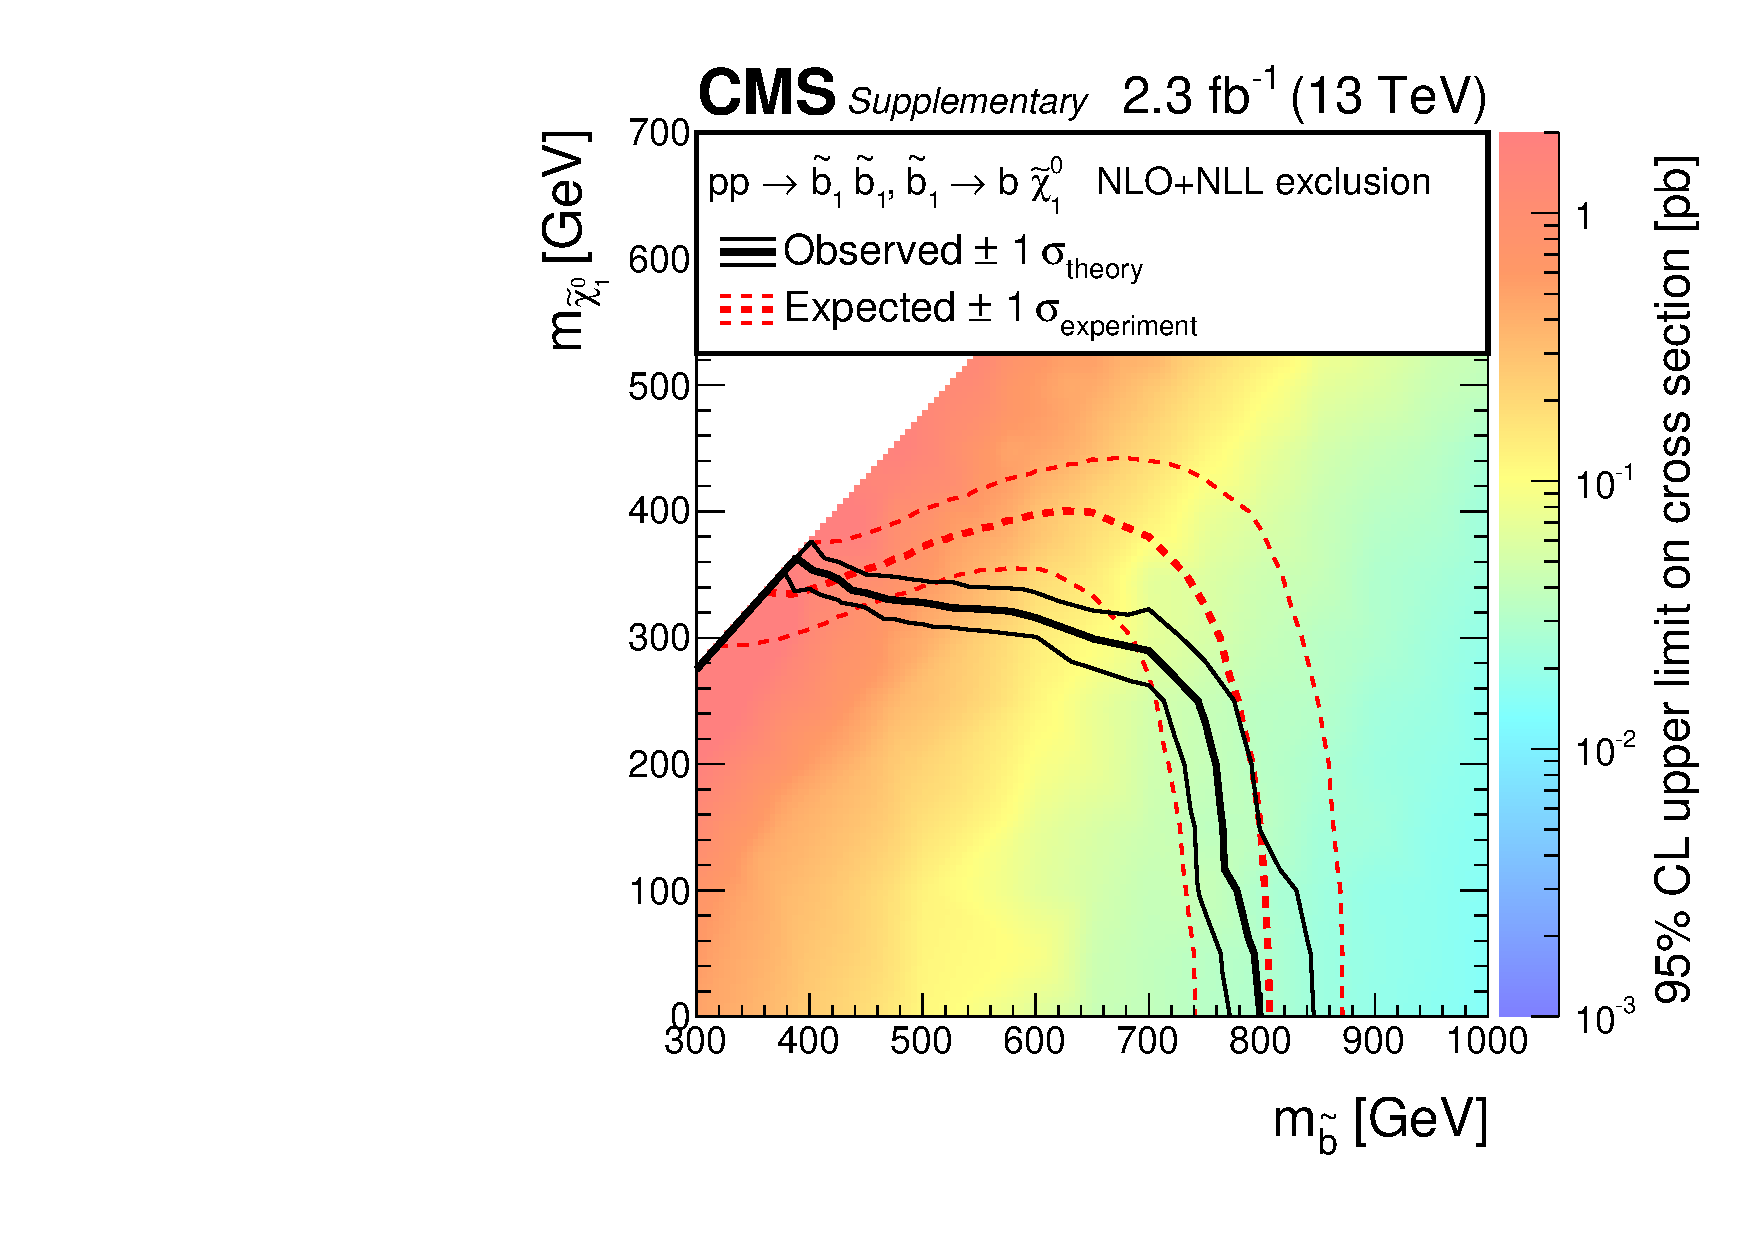
\includegraphics[width=0.49\textwidth]{Supplementary/RA1T2bbXSEC_aux} \, 
    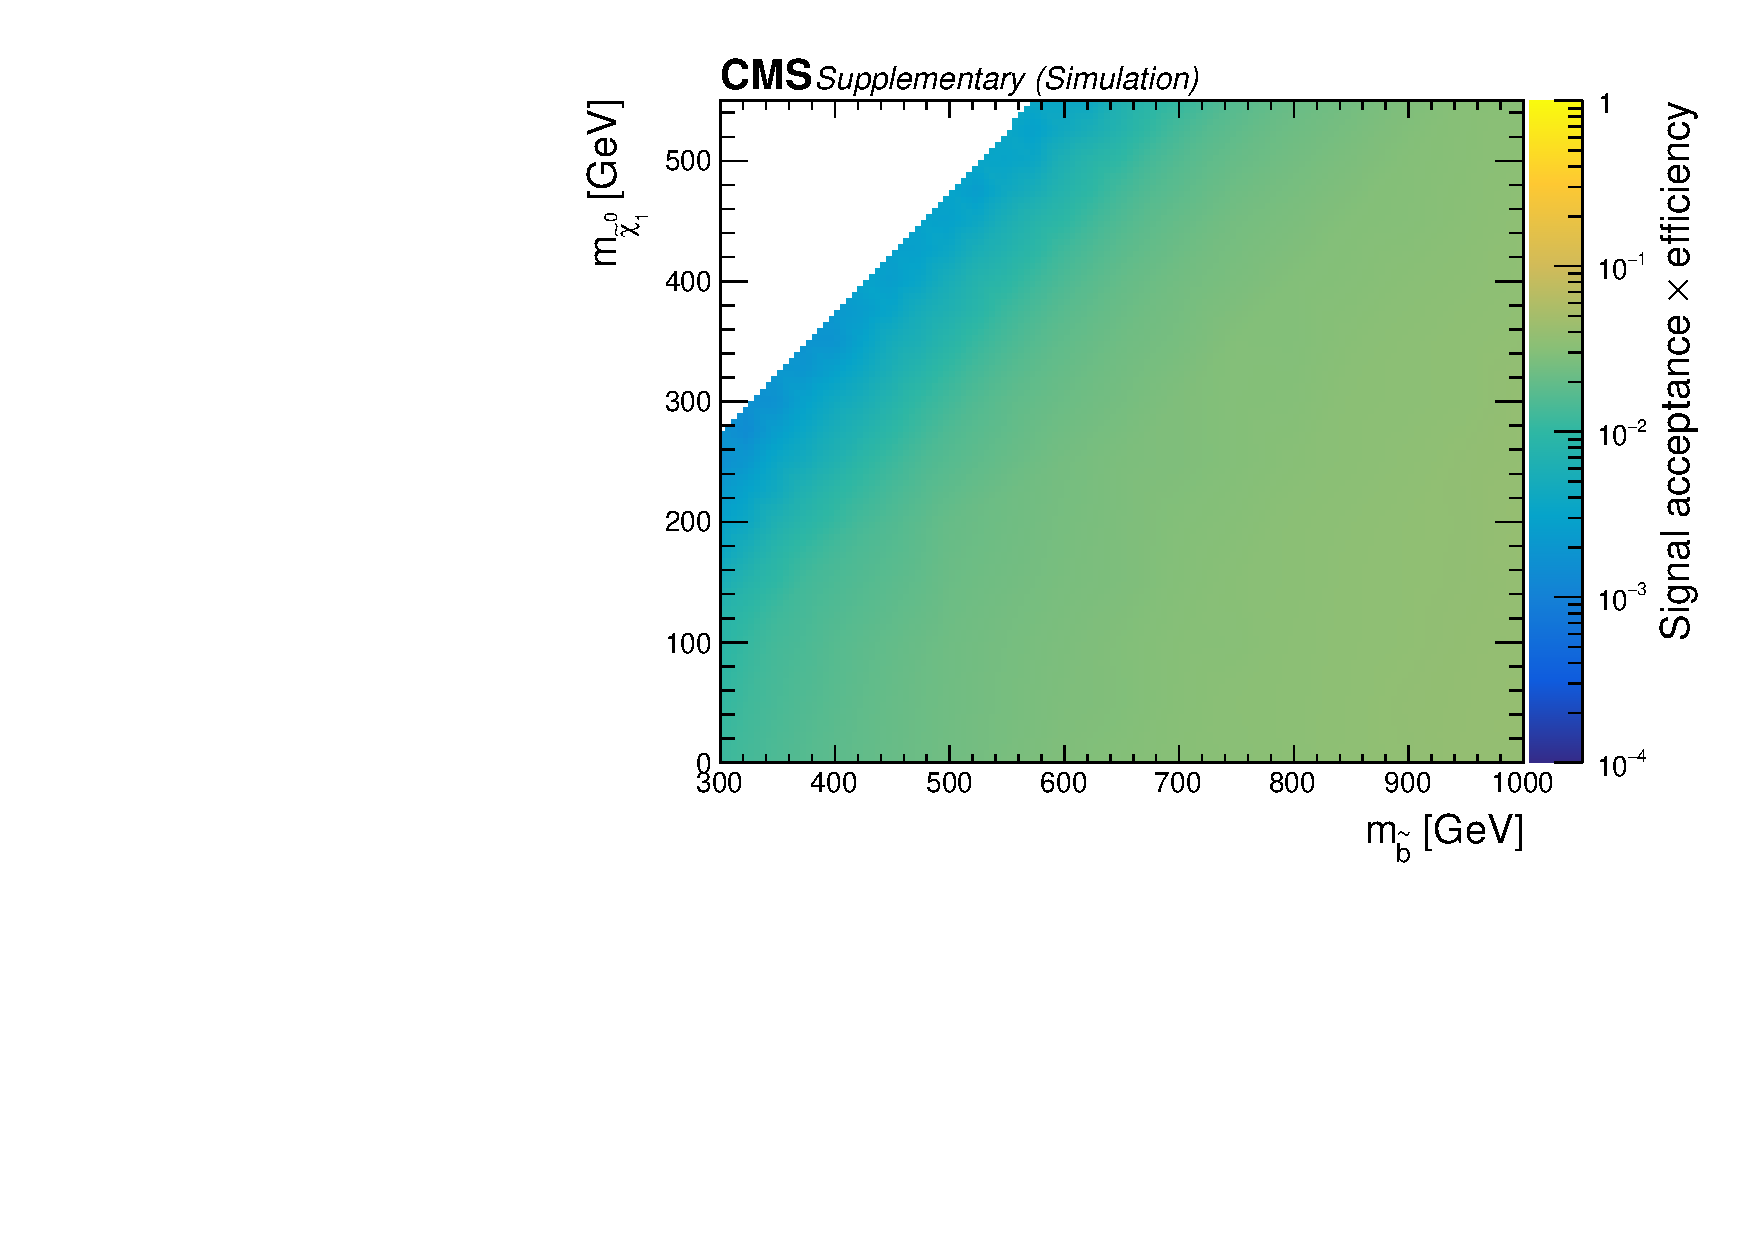
\includegraphics[width=0.49\textwidth]{Supplementary/T2bb_eff} \,     
  \end{center}
  \caption{Left: (coloured histogram) upper limit on the cross section in the $(m_{\,\PSQb}, m_{\PSGczDo})$ plane for the \texttt{T2bb} model. 
  The black (red) solid line is the observed (expected) exclusion. The red dashed lines are the $\pm1\sigma$ expected exclusion due to experimental uncertainties. 
  The $\pm1\sigma$ observed exclusion due to theoretical uncertainties on the signal cross section are shown as thin black lines. 
  Right: signal efficiency for the search regions included in the limit calculation as a function $(m_{\,\PSQb}, m_{\PSGczDo})$ plane for the \texttt{T2bb} model. 
  \label{fig:T2bb_excl}}
\end{figure*}



\clearpage
\begin{figure*}[!h]
  \begin{center}
    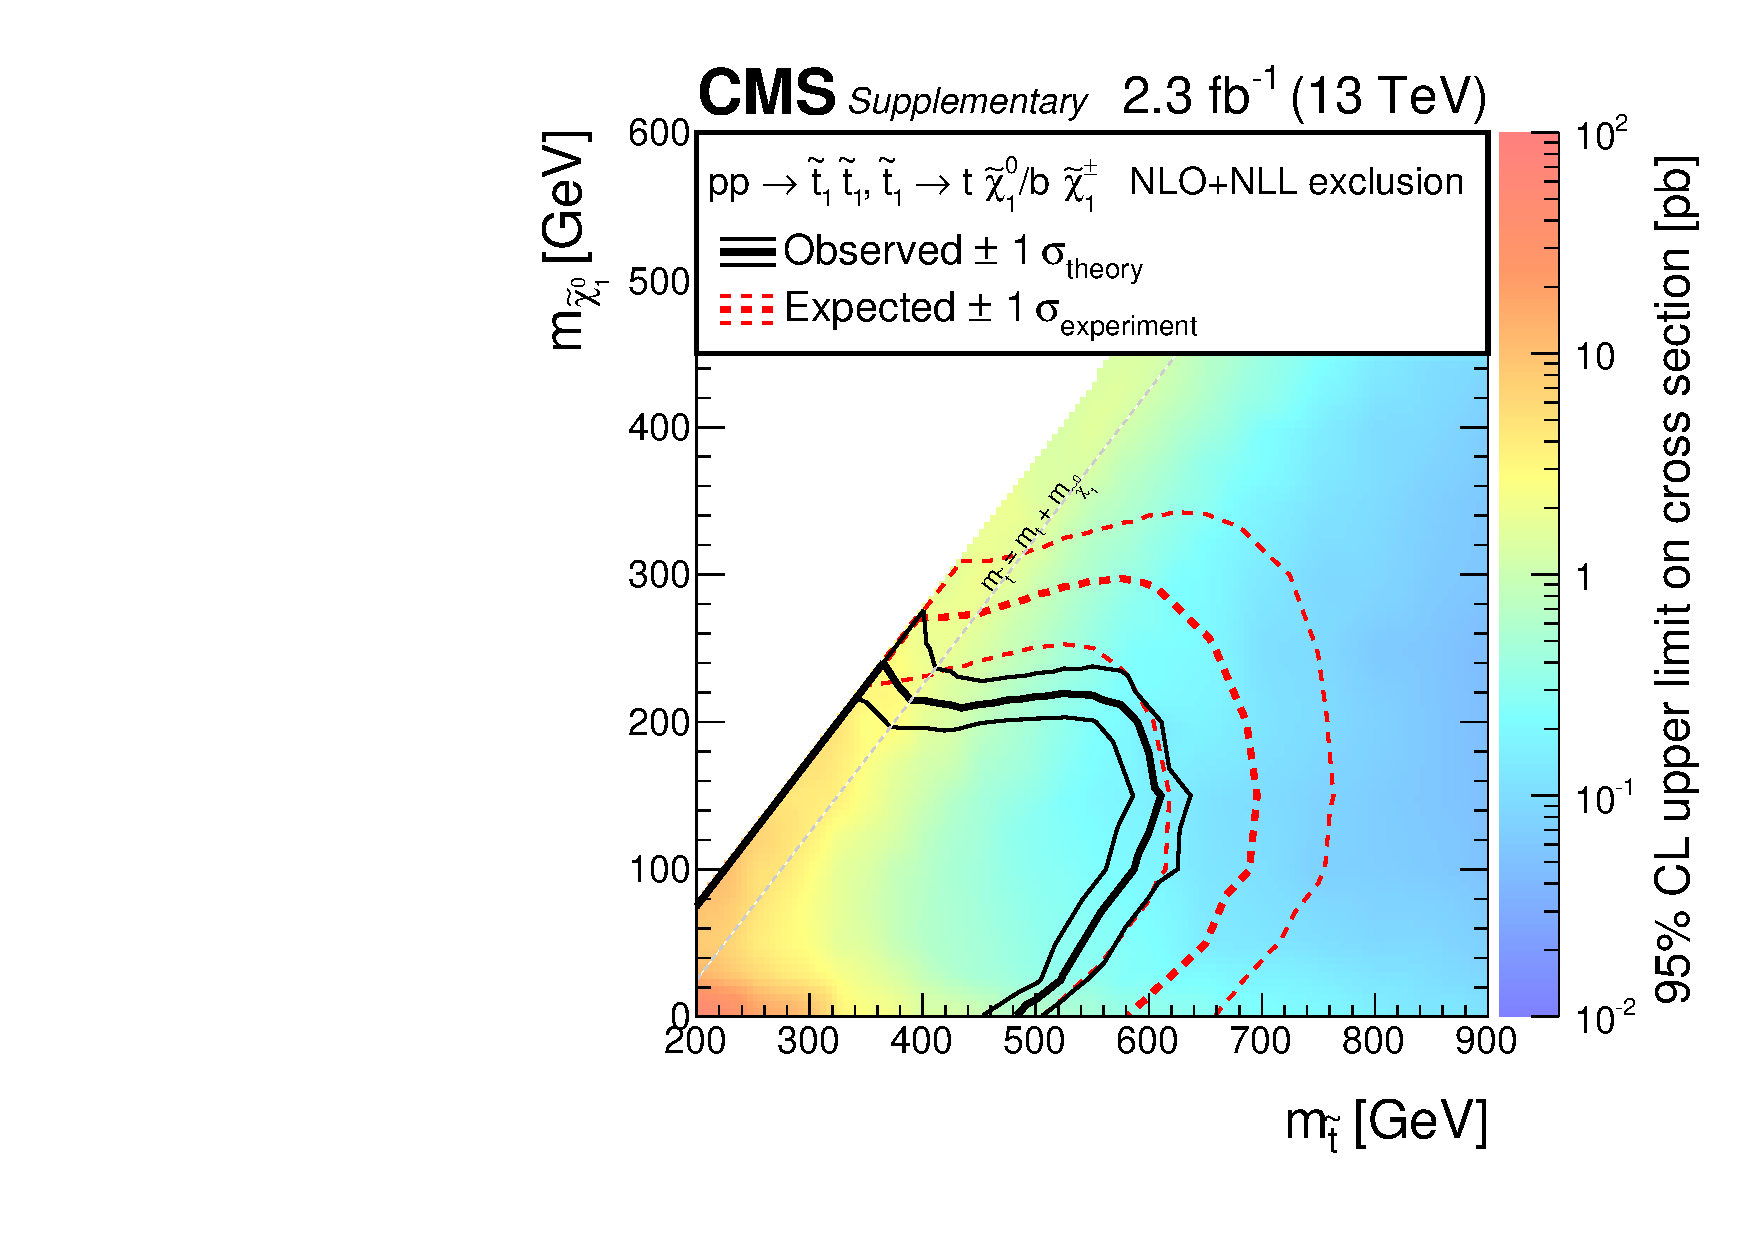
\includegraphics[width=0.49\textwidth]{Supplementary/RA1T2tbXSEC_aux} \, 
    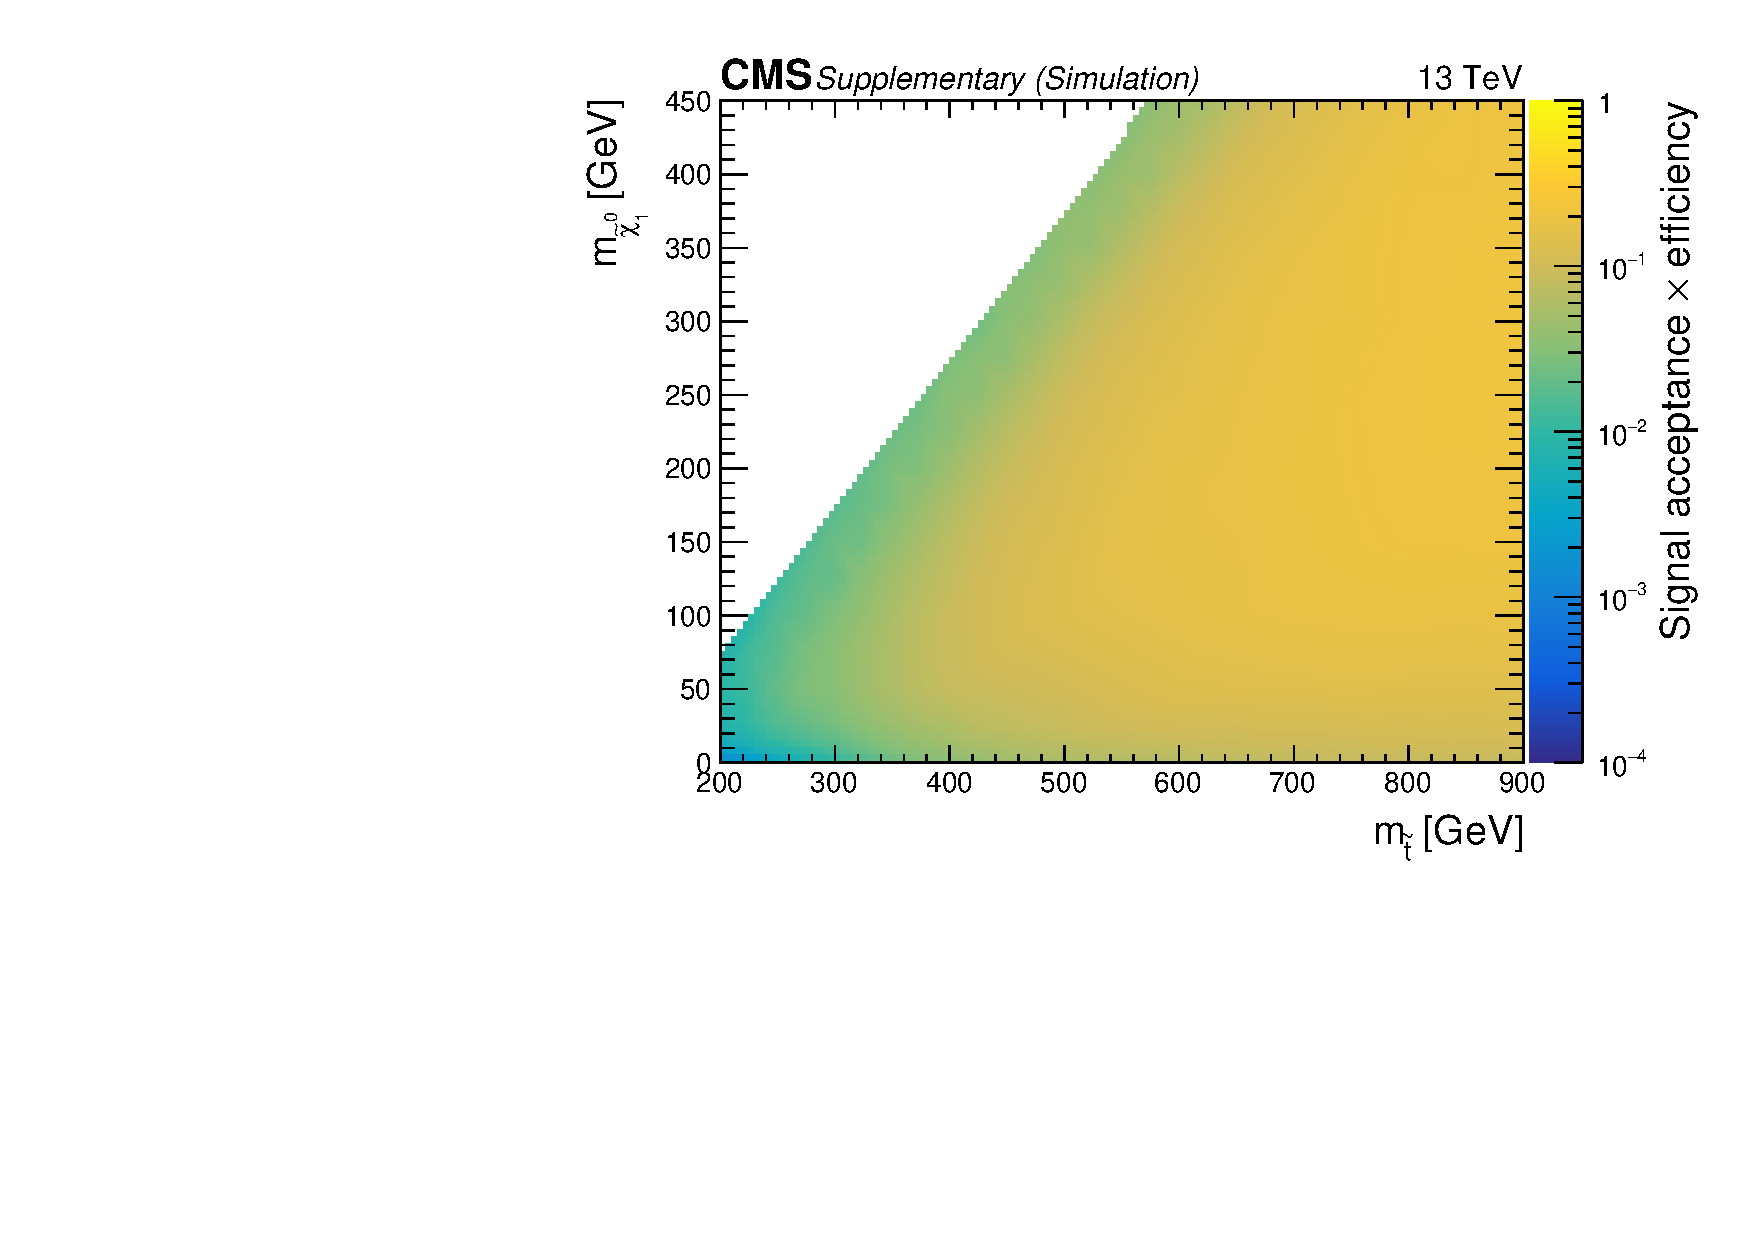
\includegraphics[width=0.49\textwidth]{Supplementary/T2tb_eff} \,     
  \end{center}
  \caption{Left: (coloured histogram) upper limit on the cross section in the $(m_{\,\PSQt}, m_{\PSGczDo})$ plane for the \texttt{T2tb} model. 
  The black (red) solid line is the observed (expected) exclusion. The red dashed lines are the $\pm1\sigma$ expected exclusion due to experimental uncertainties. 
  The $\pm1\sigma$ observed exclusion due to theoretical uncertainties on the signal cross section are shown as thin black lines. 
  Right: signal efficiency for the search regions included in the limit calculation as a function $(m_{\,\PSQt}, m_{\PSGczDo})$ plane for the \texttt{T2tb} model. 
  \label{fig:T2tb_excl}}
\end{figure*}


\clearpage
\begin{figure*}[!h]
  \begin{center}
    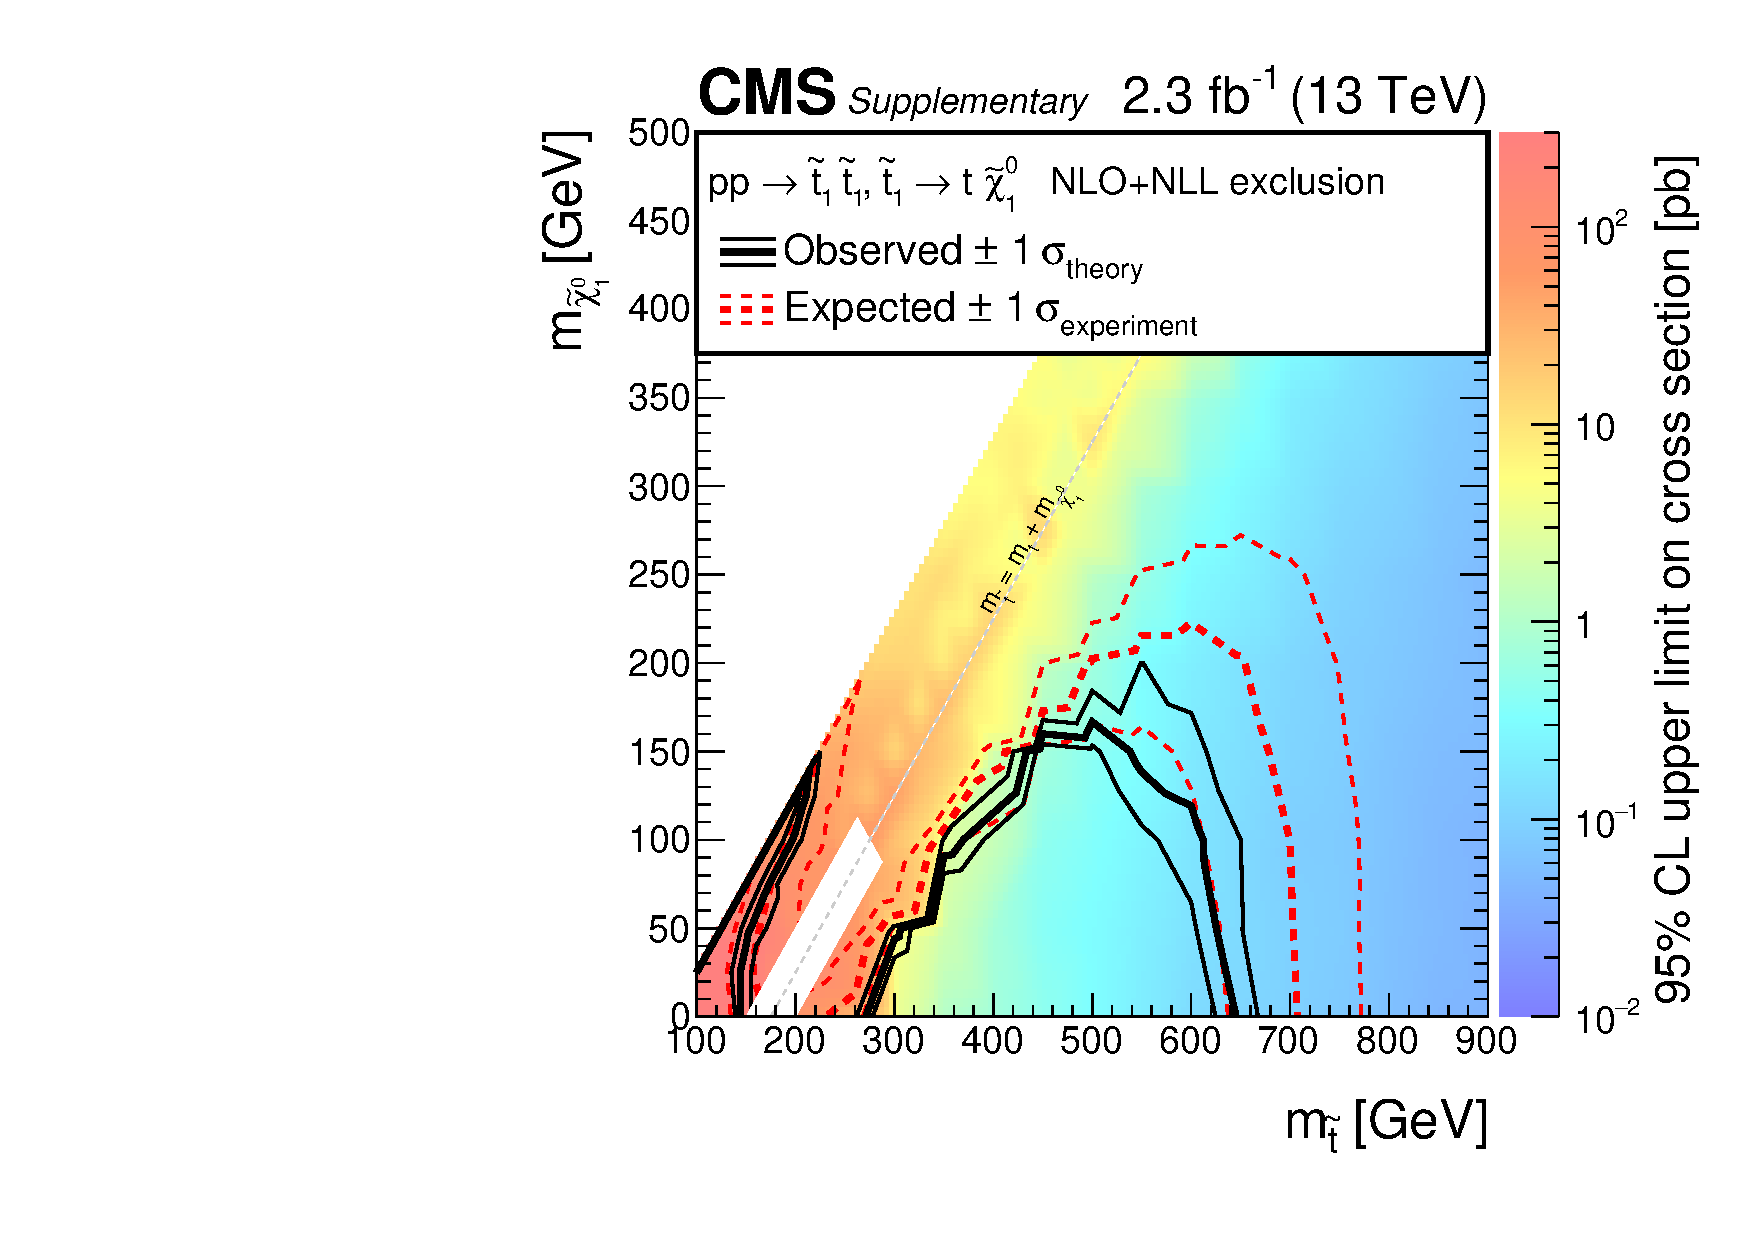
\includegraphics[width=0.49\textwidth]{Supplementary/GenMetXSEC_aux} \, % was RA1T2ttXSEC
    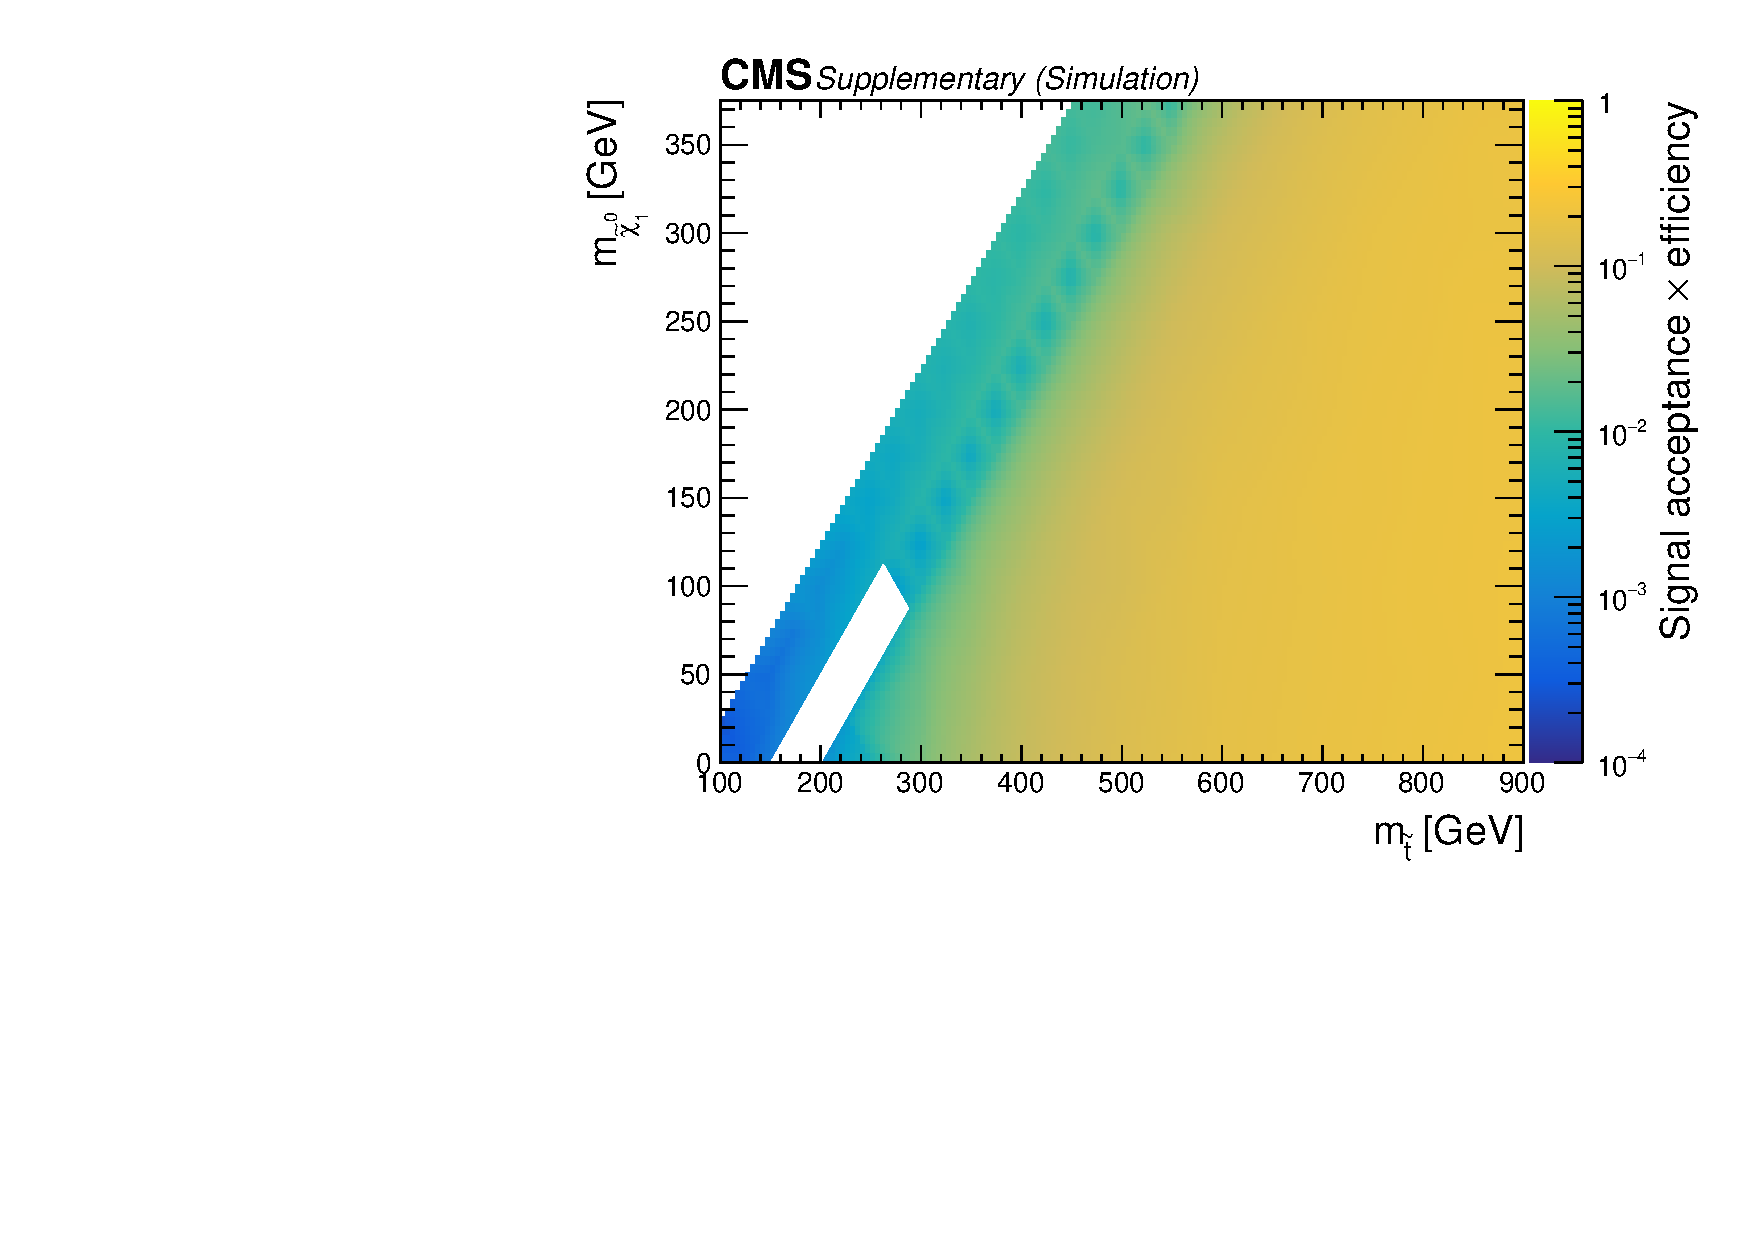
\includegraphics[width=0.49\textwidth]{Supplementary/T2tt_eff} \,     
  \end{center}
  \caption{Left: (coloured histogram) upper limit on the cross section in the $(m_{\,\PSQt}, m_{\PSGczDo})$ plane for the \texttt{T2tt} model. 
  The black (red) solid line is the observed (expected) exclusion. The red dashed lines are the $\pm1\sigma$ expected exclusion due to experimental uncertainties. 
  The $\pm1\sigma$ observed exclusion due to theoretical uncertainties on the signal cross section are shown as thin black lines. 
  Right: signal efficiency for the search regions included in the limit calculation as a function $(m_{\,\PSQt}, m_{\PSGczDo})$ plane for the \texttt{T2tt} model. 
  \label{fig:T2tt_excl}}
\end{figure*}


\clearpage
\begin{figure*}[!h]
  \begin{center}
    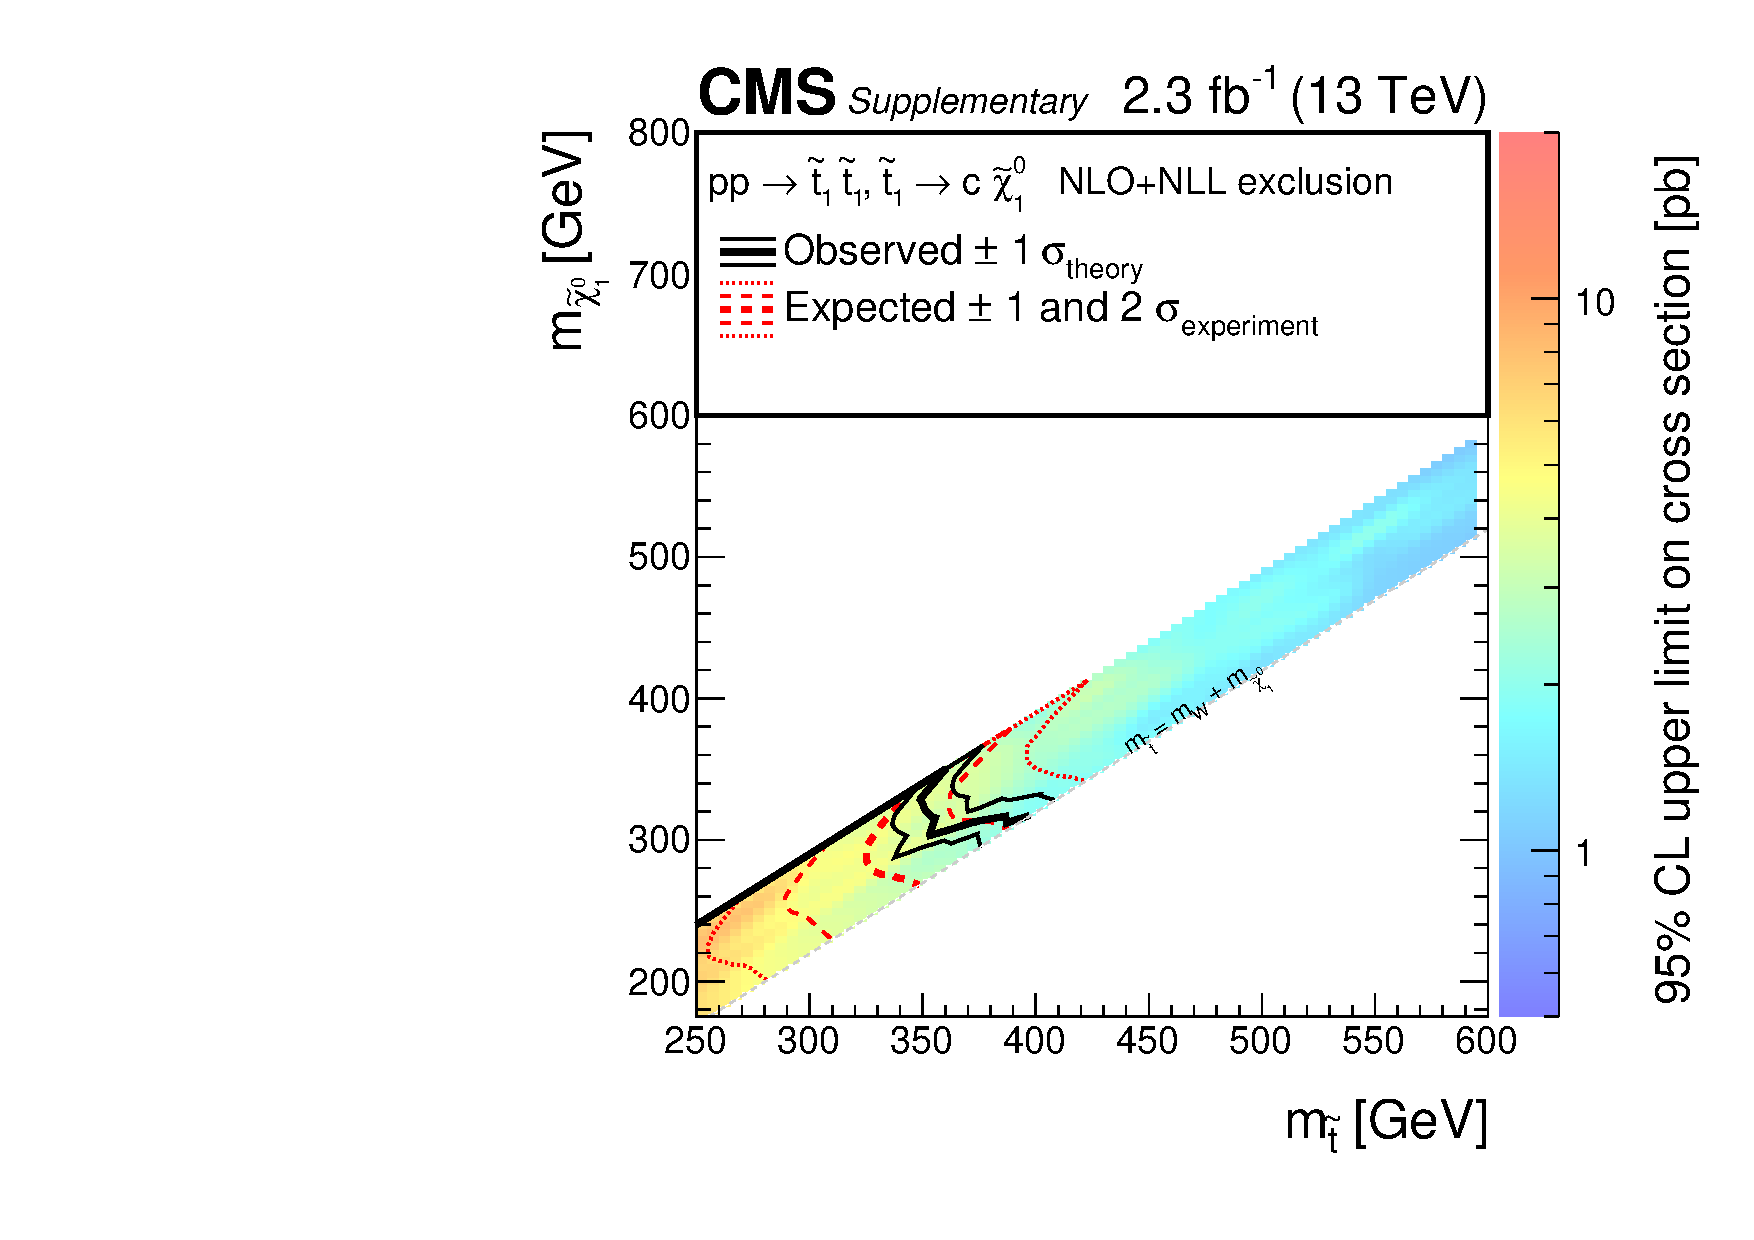
\includegraphics[width=0.49\textwidth]{Supplementary/RA1T2ccXSEC_aux} \, 
    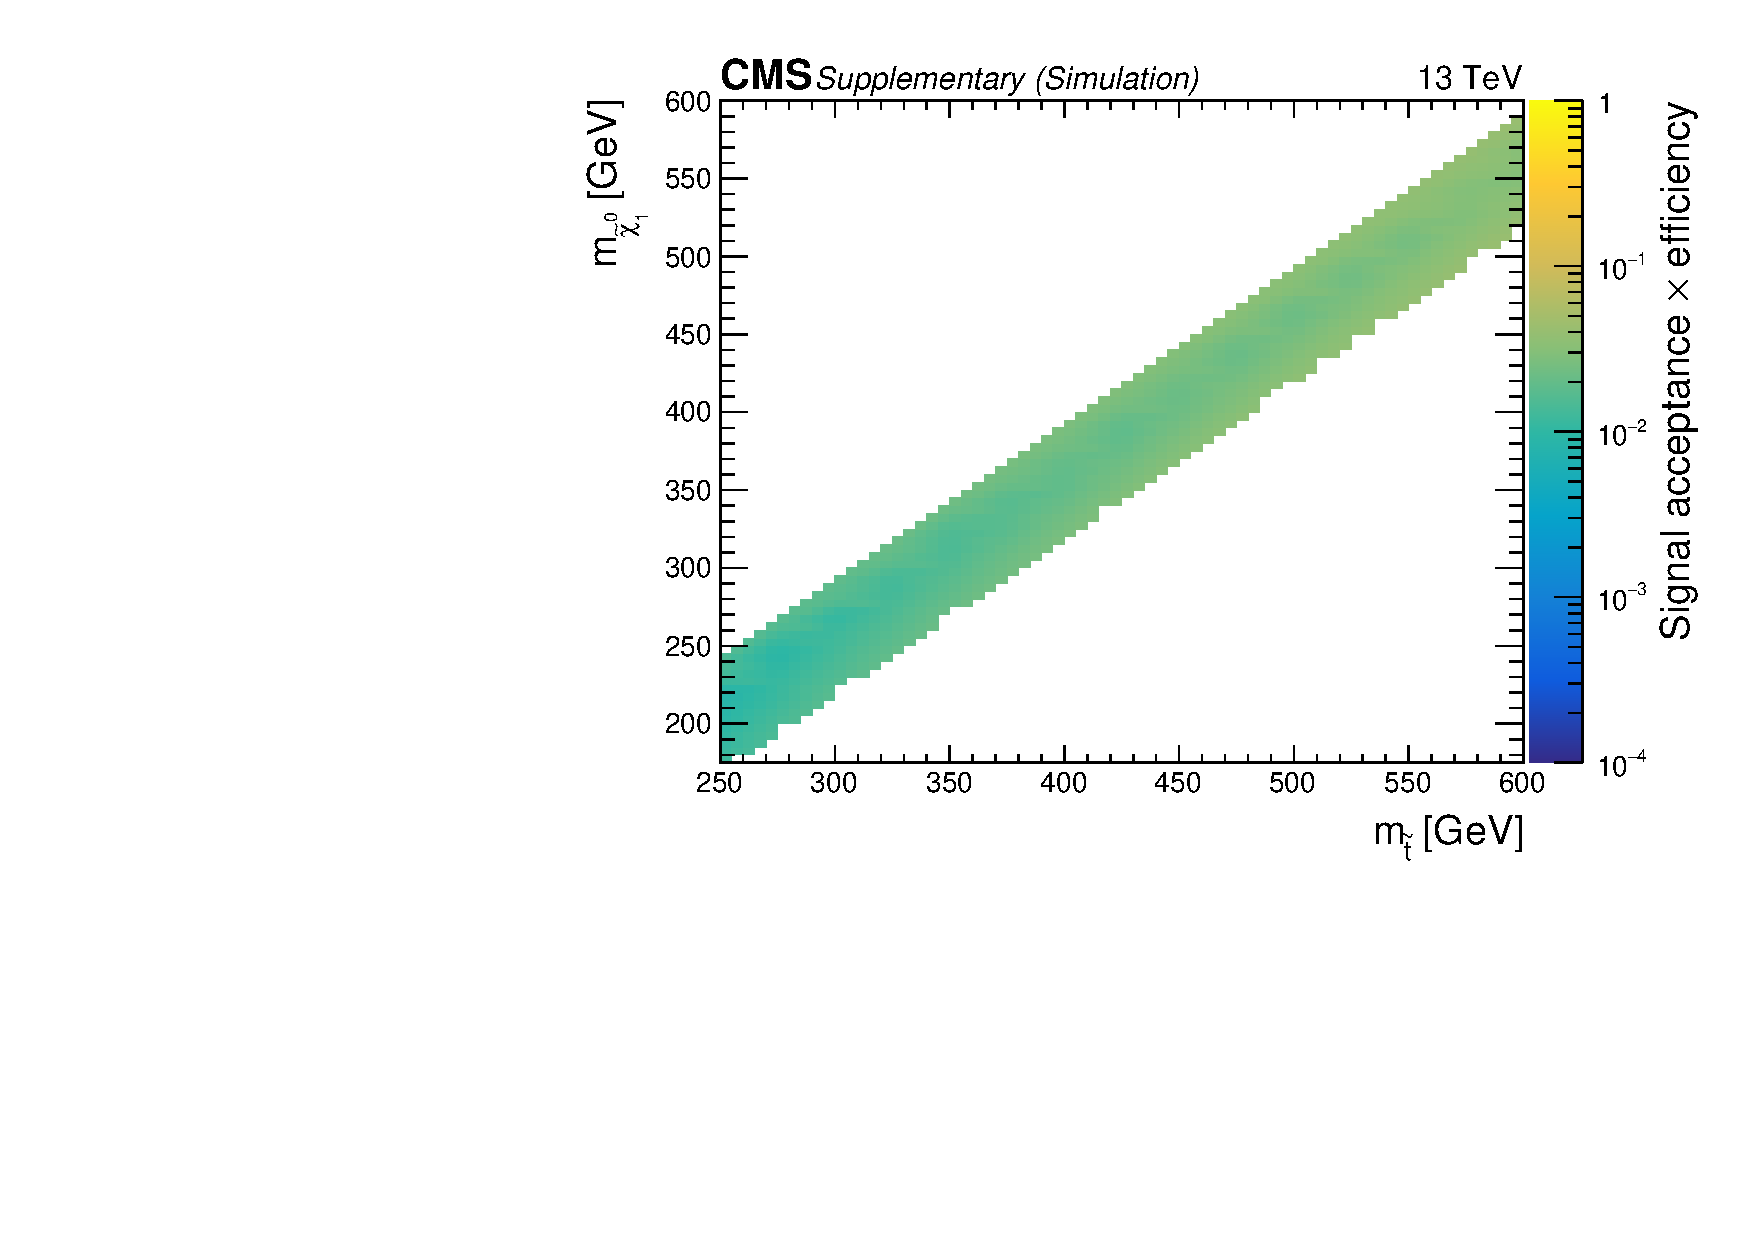
\includegraphics[width=0.49\textwidth]{Supplementary/T2cc_eff} \,     
  \end{center}
  \caption{Left: (coloured histogram) upper limit on the cross section in the $(m_{\,\PSQt}, m_{\PSGczDo})$ plane for the \texttt{T2cc} model. 
  The black (red) solid line is the observed (expected) exclusion. The red dashed lines are the $\pm1\sigma$ expected exclusion due to experimental uncertainties. 
  The $\pm1\sigma$ observed exclusion due to theoretical uncertainties on the signal cross section are shown as thin black lines. 
  Right: signal efficiency for the search regions included in the limit calculation as a function $(m_{\,\PSQt}, m_{\PSGczDo})$ plane for the \texttt{T2cc} model. 
  \label{fig:T2cc_excl}}
\end{figure*}


\clearpage
\begin{figure*}[!h]
  \begin{center}
    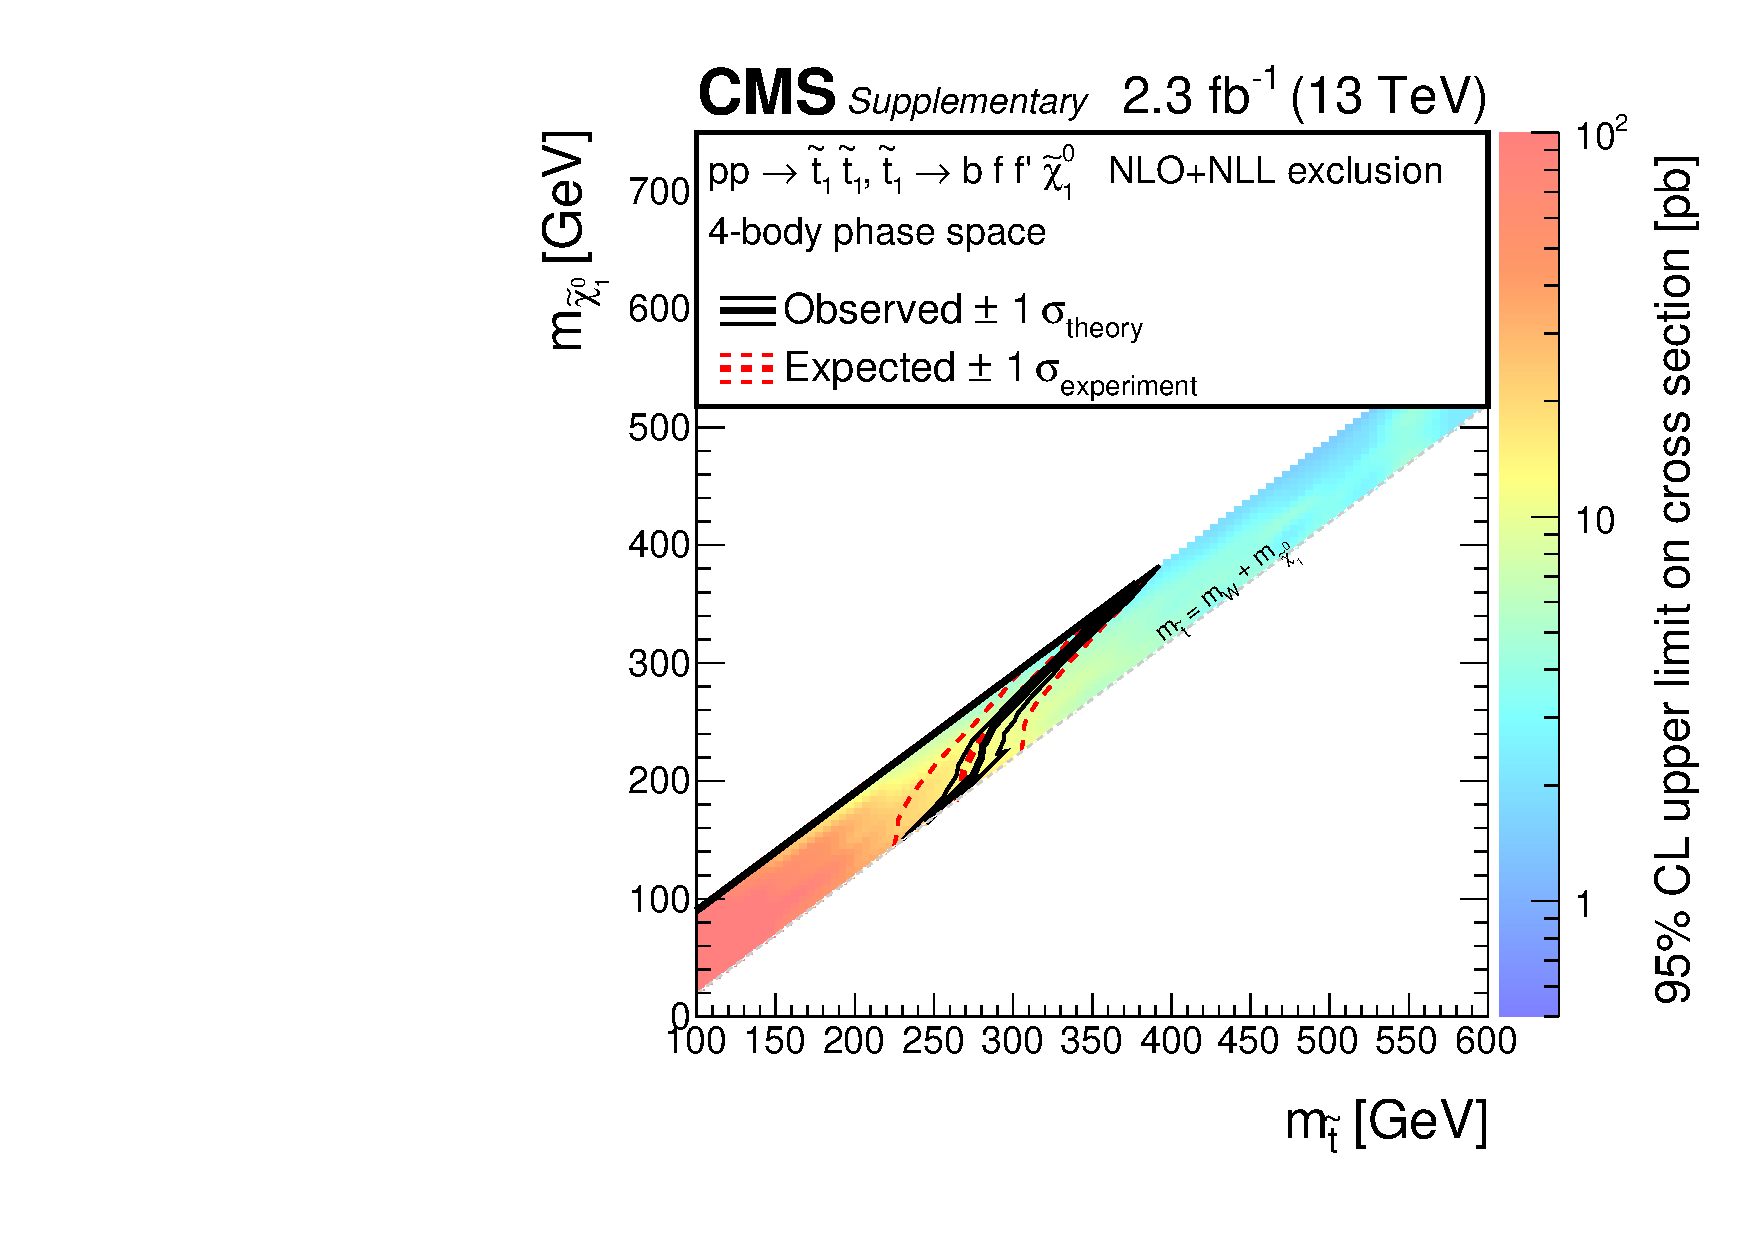
\includegraphics[width=0.49\textwidth]{Supplementary/RA1T2-4bdXSEC_aux} \, 
    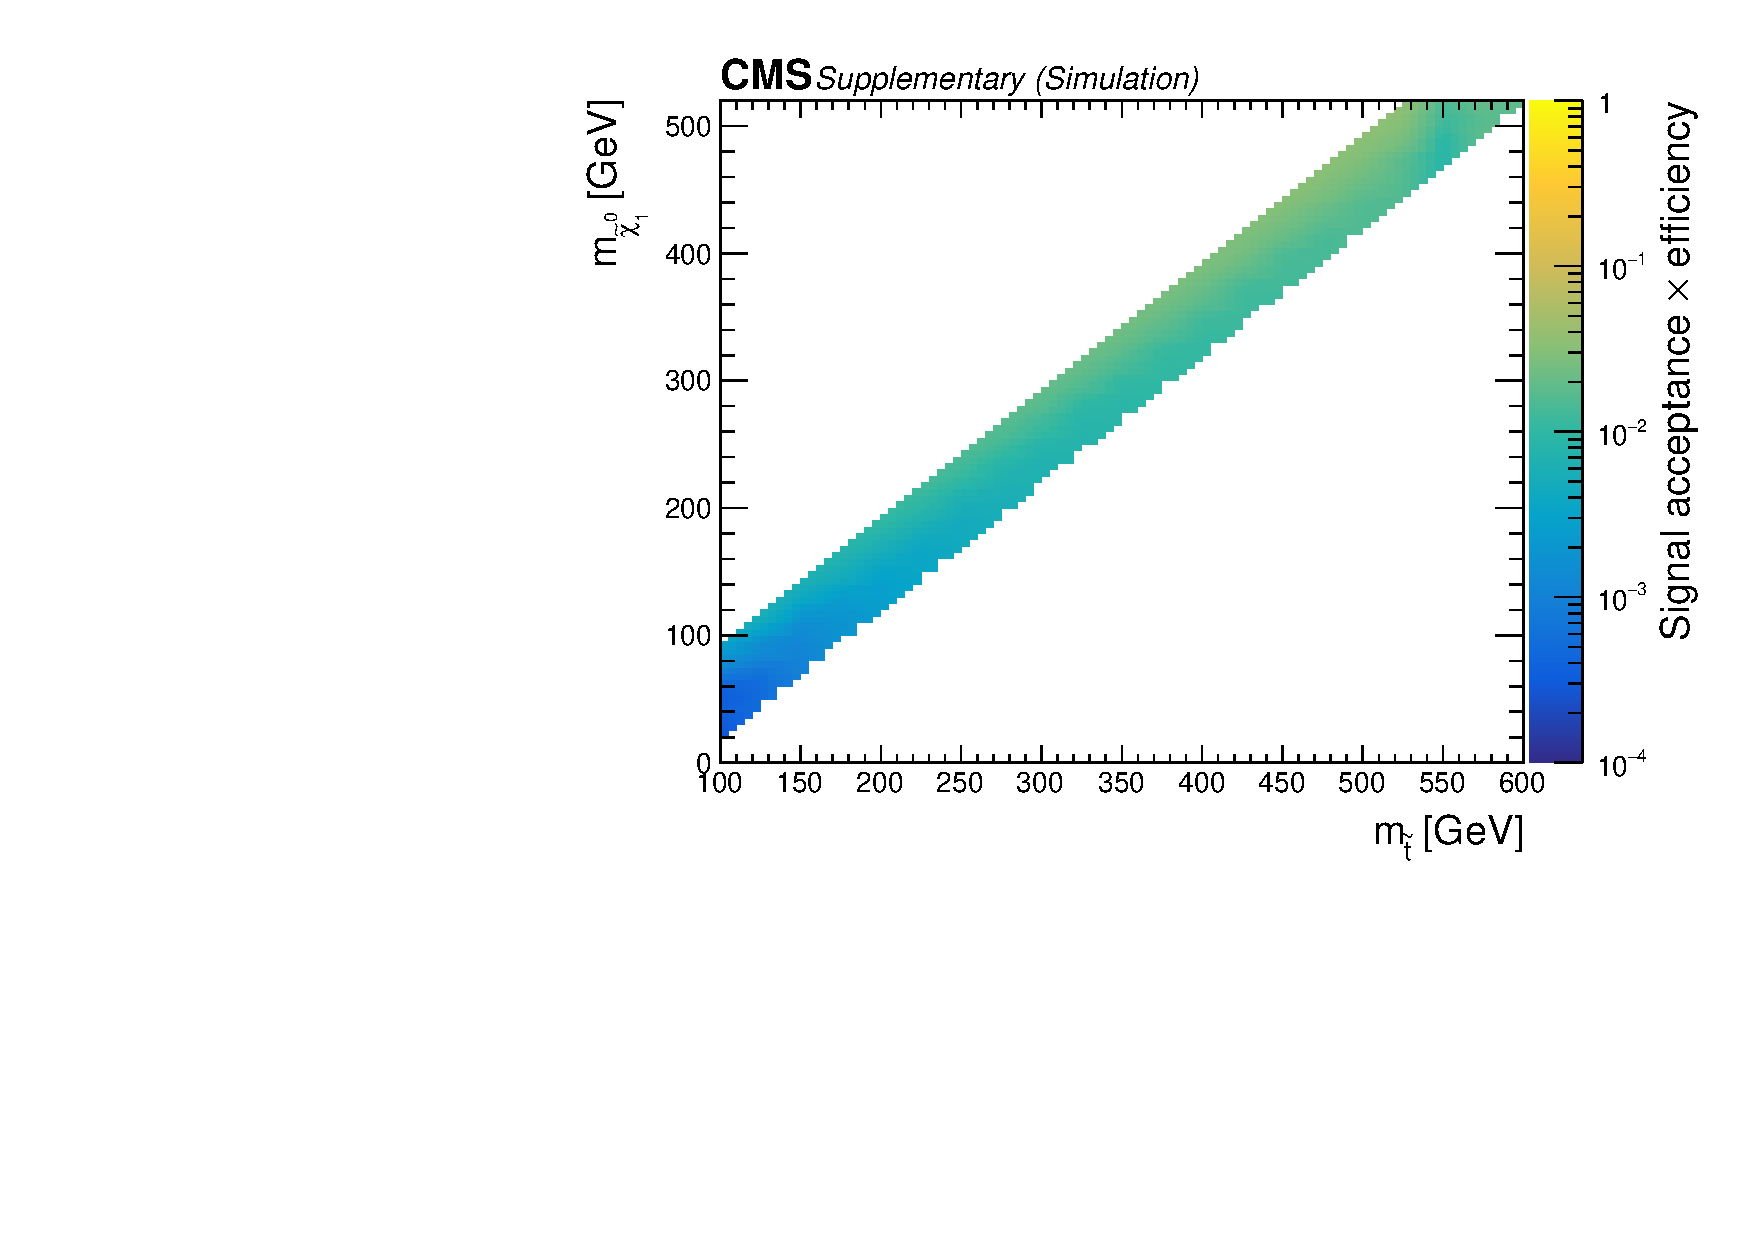
\includegraphics[width=0.49\textwidth]{Supplementary/T2-4bd_eff} \,     
  \end{center}
  \caption{Left: (coloured histogram) upper limit on the cross section in the $(m_{\,\PSQt}, m_{\PSGczDo})$ plane for the \texttt{T2tt\_degen} model. 
  The black (red) solid line is the observed (expected) exclusion. The red dashed lines are the $\pm1\sigma$ expected exclusion due to experimental uncertainties. 
  The $\pm1\sigma$ observed exclusion due to theoretical uncertainties on the signal cross section are shown as thin black lines. 
  Right: signal efficiency for the search regions included in the limit calculation as a function $(m_{\,\PSQt}, m_{\PSGczDo})$ plane for the \texttt{T2tt\_degen} model. 
  \label{fig:T2-4bd_excl}}
\end{figure*}


\clearpage
\begin{figure*}[!h]
  \begin{center}
    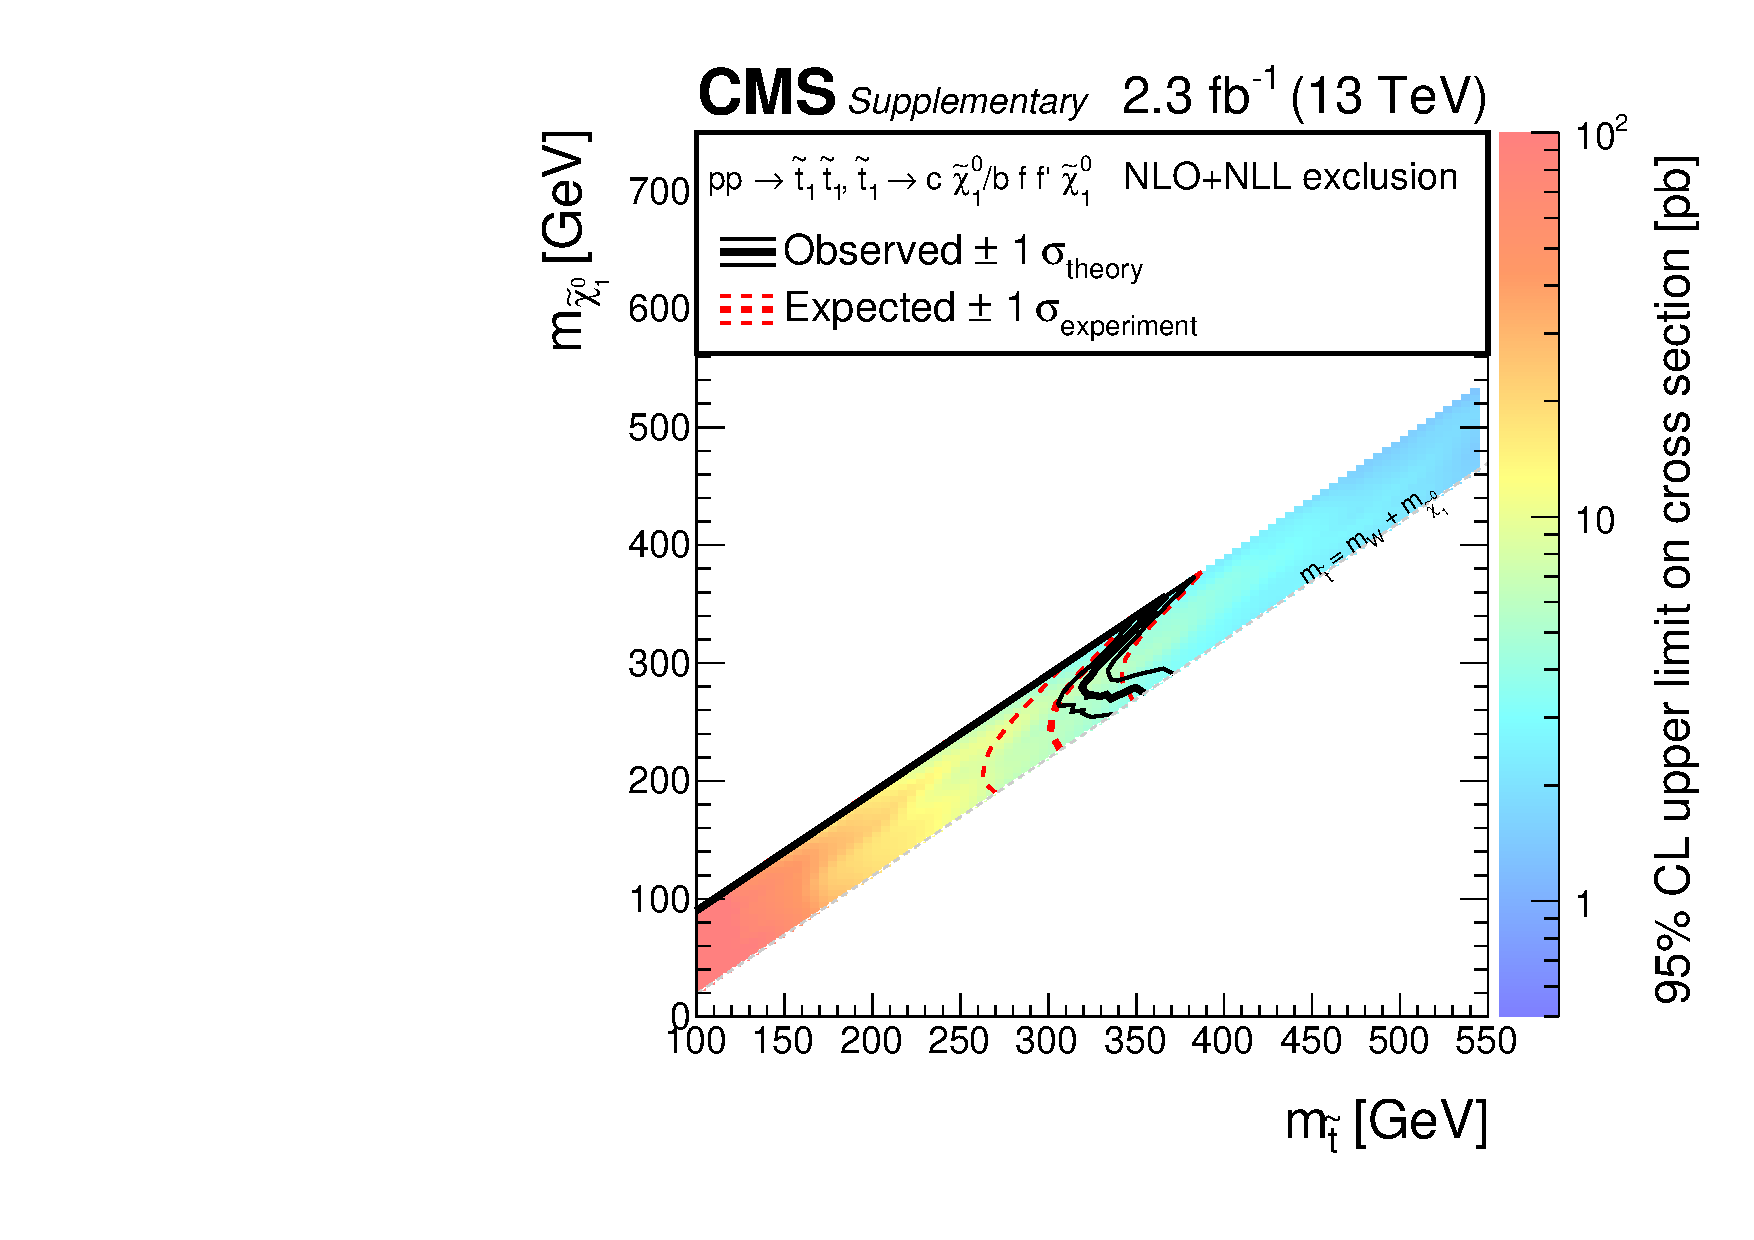
\includegraphics[width=0.49\textwidth]{Supplementary/RA1T2mixedXSEC_aux} \, 
    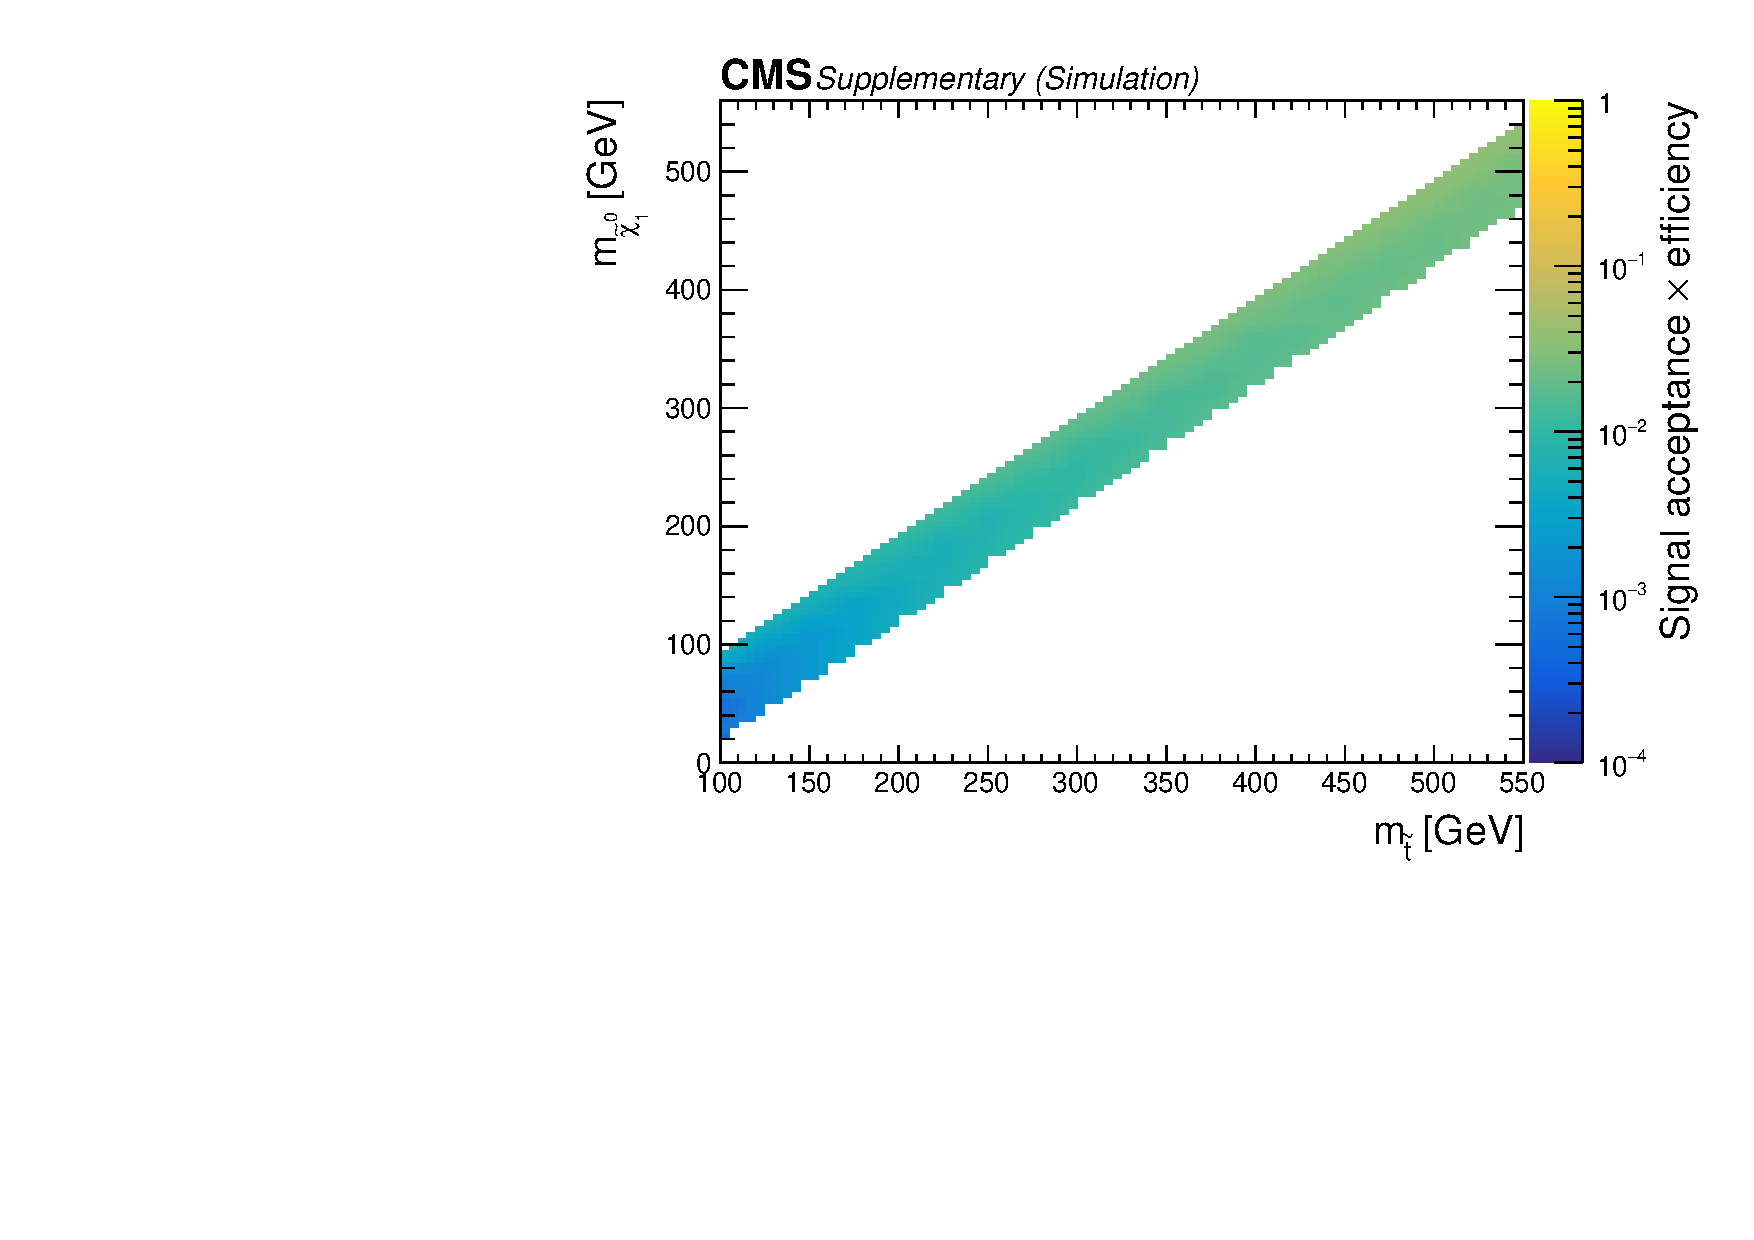
\includegraphics[width=0.49\textwidth]{Supplementary/T2mixed_eff} \,     
  \end{center}
  \caption{Left: (coloured histogram) upper limit on the cross section in the $(m_{\,\PSQt}, m_{\PSGczDo})$ plane for the \texttt{T2\_mixed} model. 
  The black (red) solid line is the observed (expected) exclusion. The red dashed lines are the $\pm1\sigma$ expected exclusion due to experimental uncertainties. 
  The $\pm1\sigma$ observed exclusion due to theoretical uncertainties on the signal cross section are shown as thin black lines. 
  Right: signal efficiency for the search regions included in the limit calculation as a function $(m_{\,\PSQt}, m_{\PSGczDo})$ plane for the \texttt{T2\_mixed} model. 
  \label{fig:T2mixed_excl}}
\end{figure*}



\clearpage
\begin{figure*}[!h]
  \begin{center}
    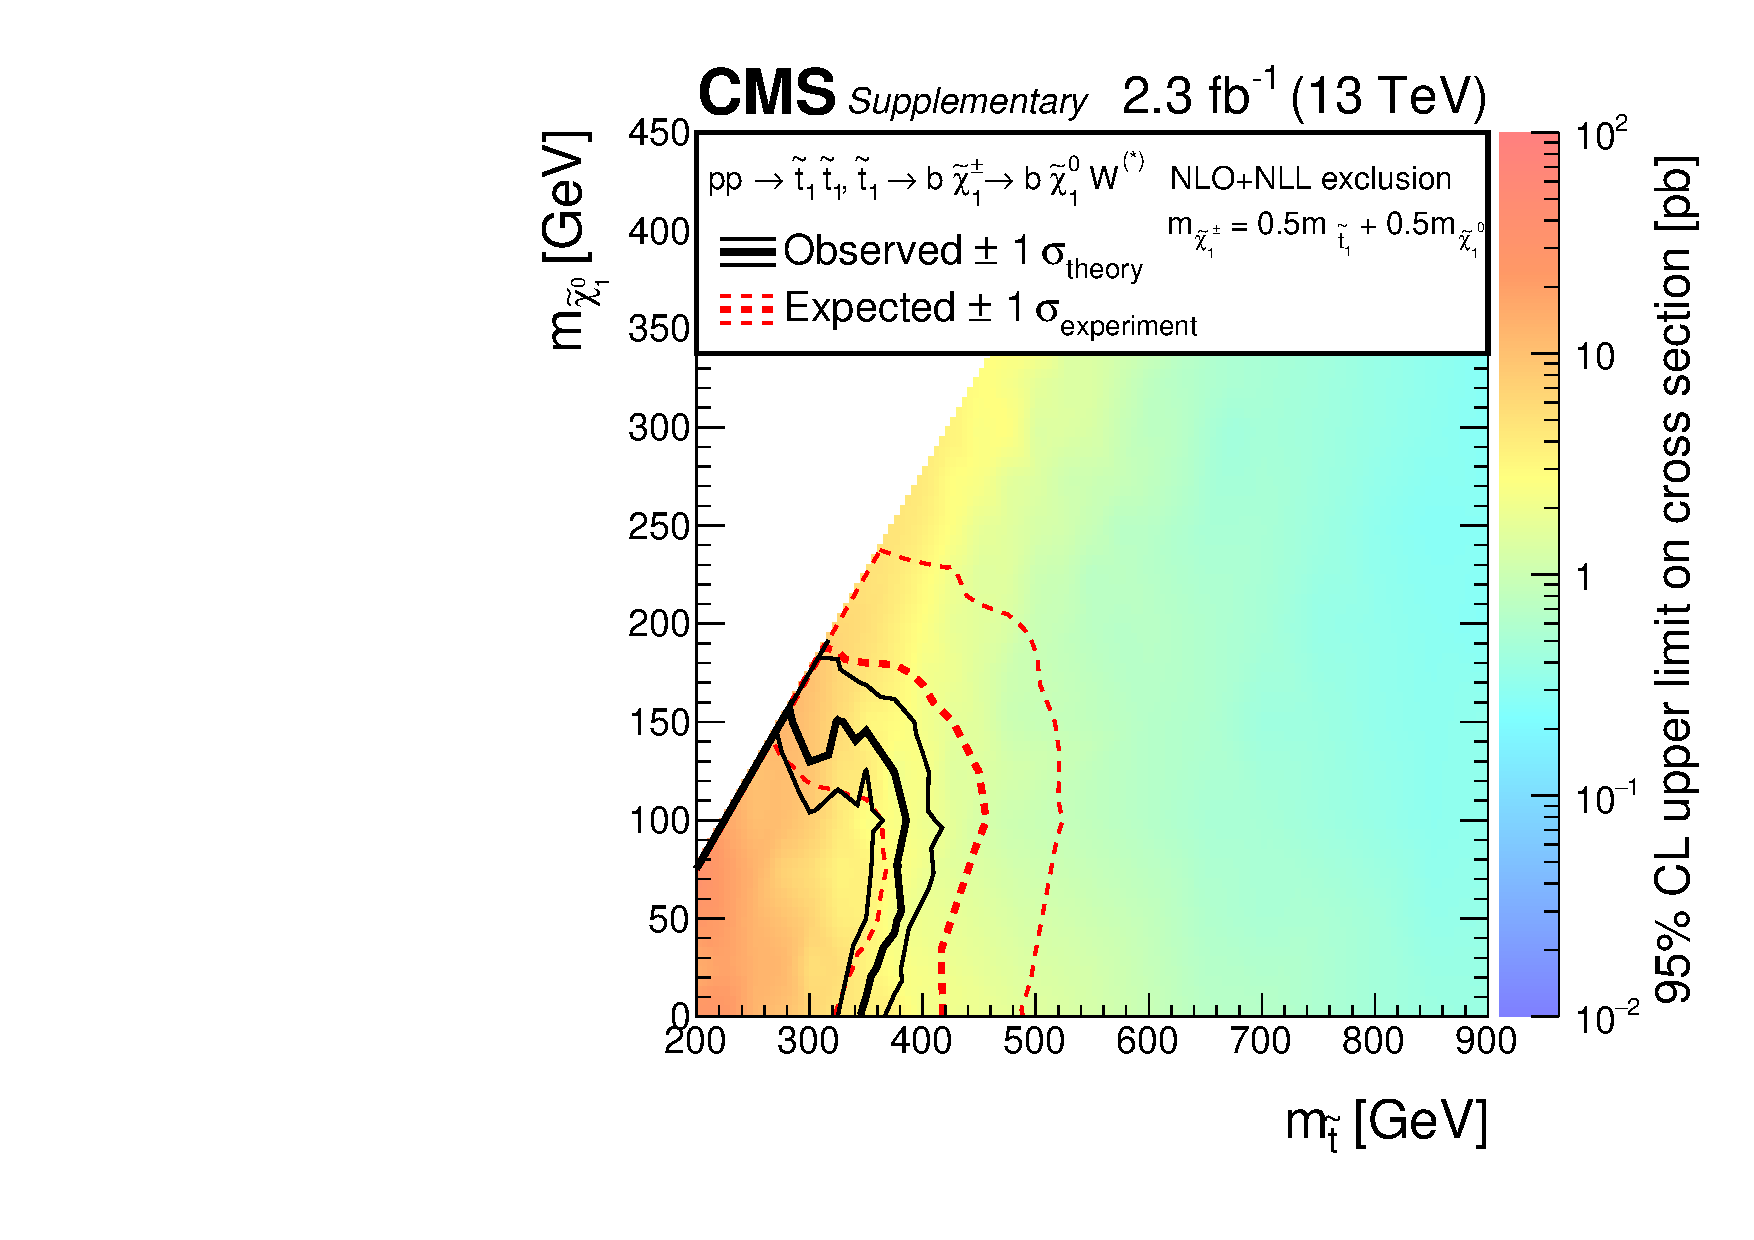
\includegraphics[width=0.49\textwidth]{Supplementary/RA1T2bW-X05XSEC_aux} \, 
    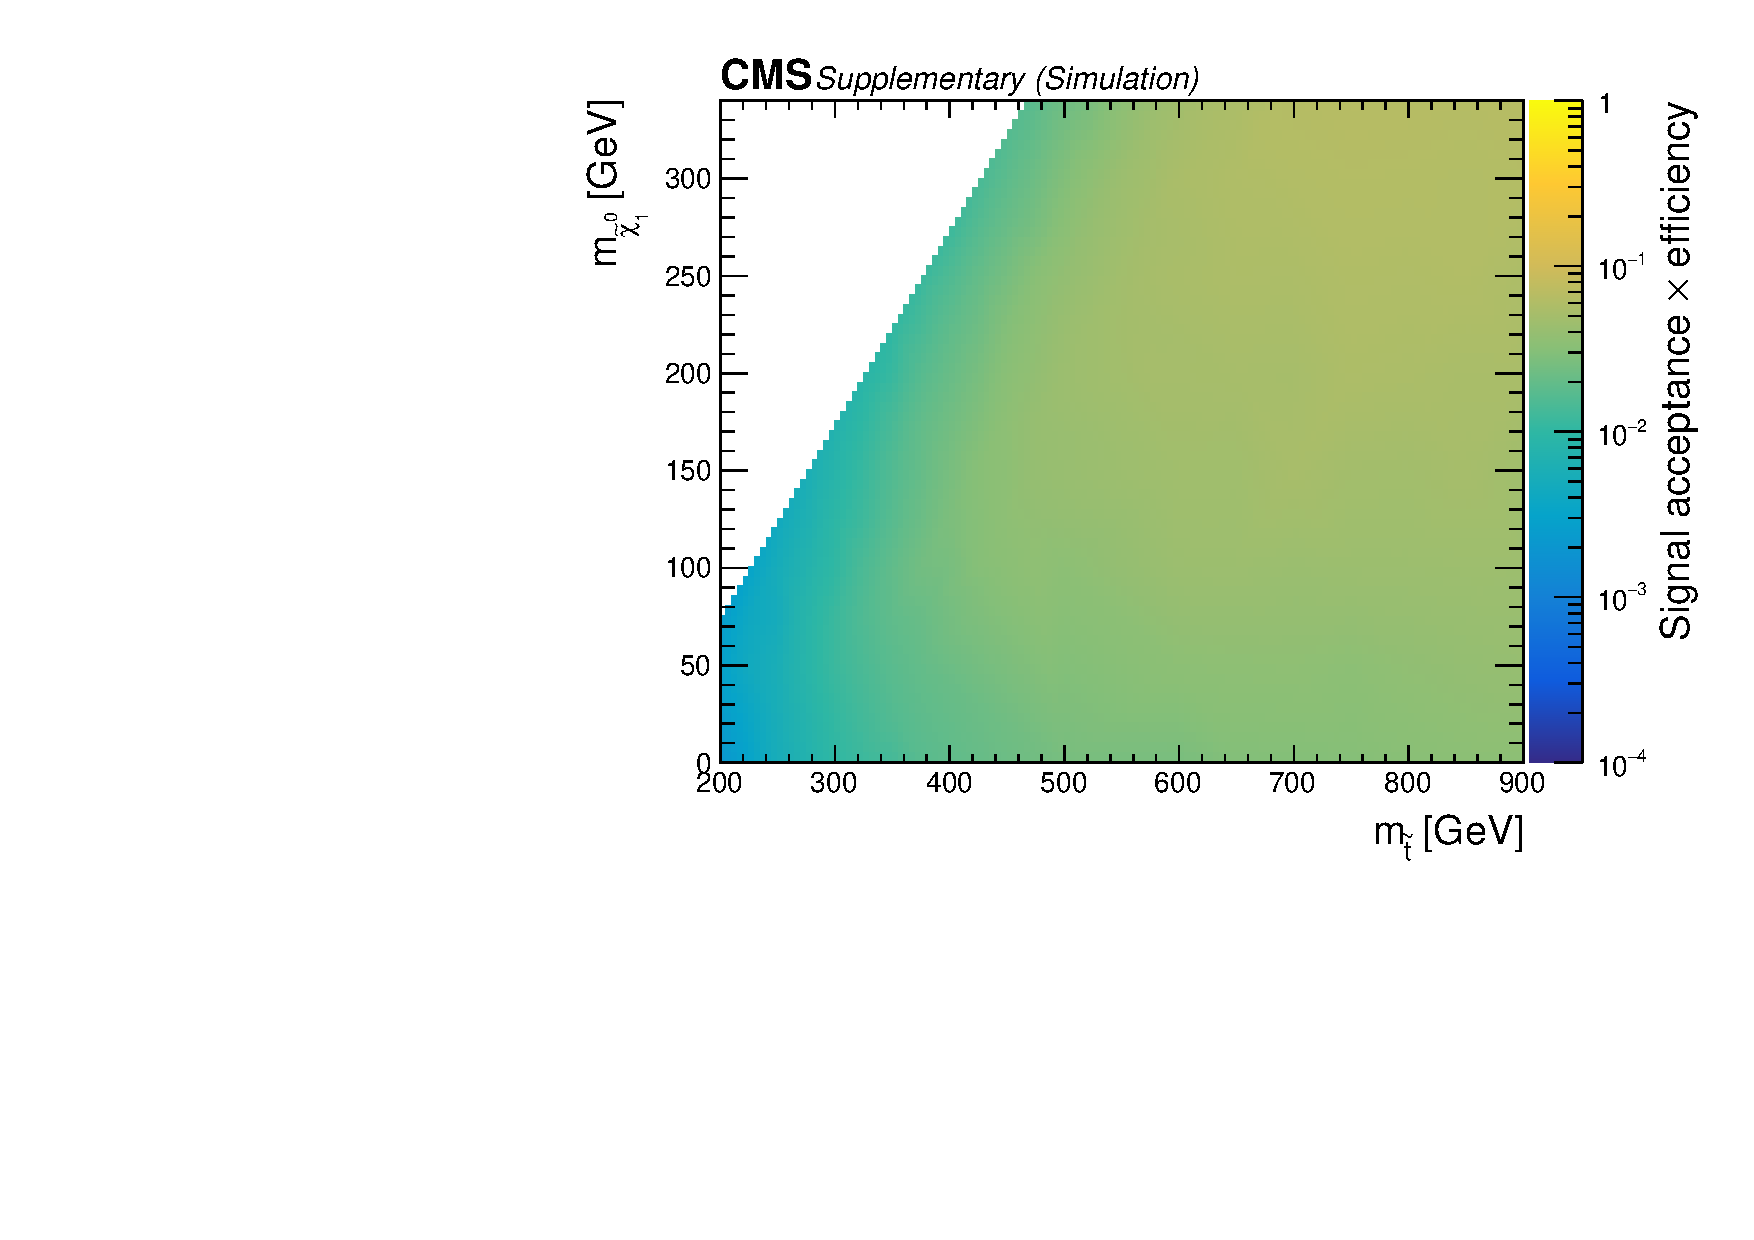
\includegraphics[width=0.49\textwidth]{Supplementary/T2bW_X05_eff} \,     
  \end{center}
  \caption{Left: (coloured histogram) upper limit on the cross section in the $(m_{\,\PSQt}, m_{\PSGczDo})$ plane for the \texttt{T2bW} model. 
  The black (red) solid line is the observed (expected) exclusion. The red dashed lines are the $\pm1\sigma$ expected exclusion due to experimental uncertainties. 
  The $\pm1\sigma$ observed exclusion due to theoretical uncertainties on the signal cross section are shown as thin black lines. 
  Right: signal efficiency for the search regions included in the limit calculation as a function $(m_{\,\PSQt}, m_{\PSGczDo})$ plane for the \texttt{T2bW} model. 
  \label{fig:T2bW_X05_excl}}
\end{figure*}

\clearpage
\begin{figure*}[!h]
  \begin{center}
    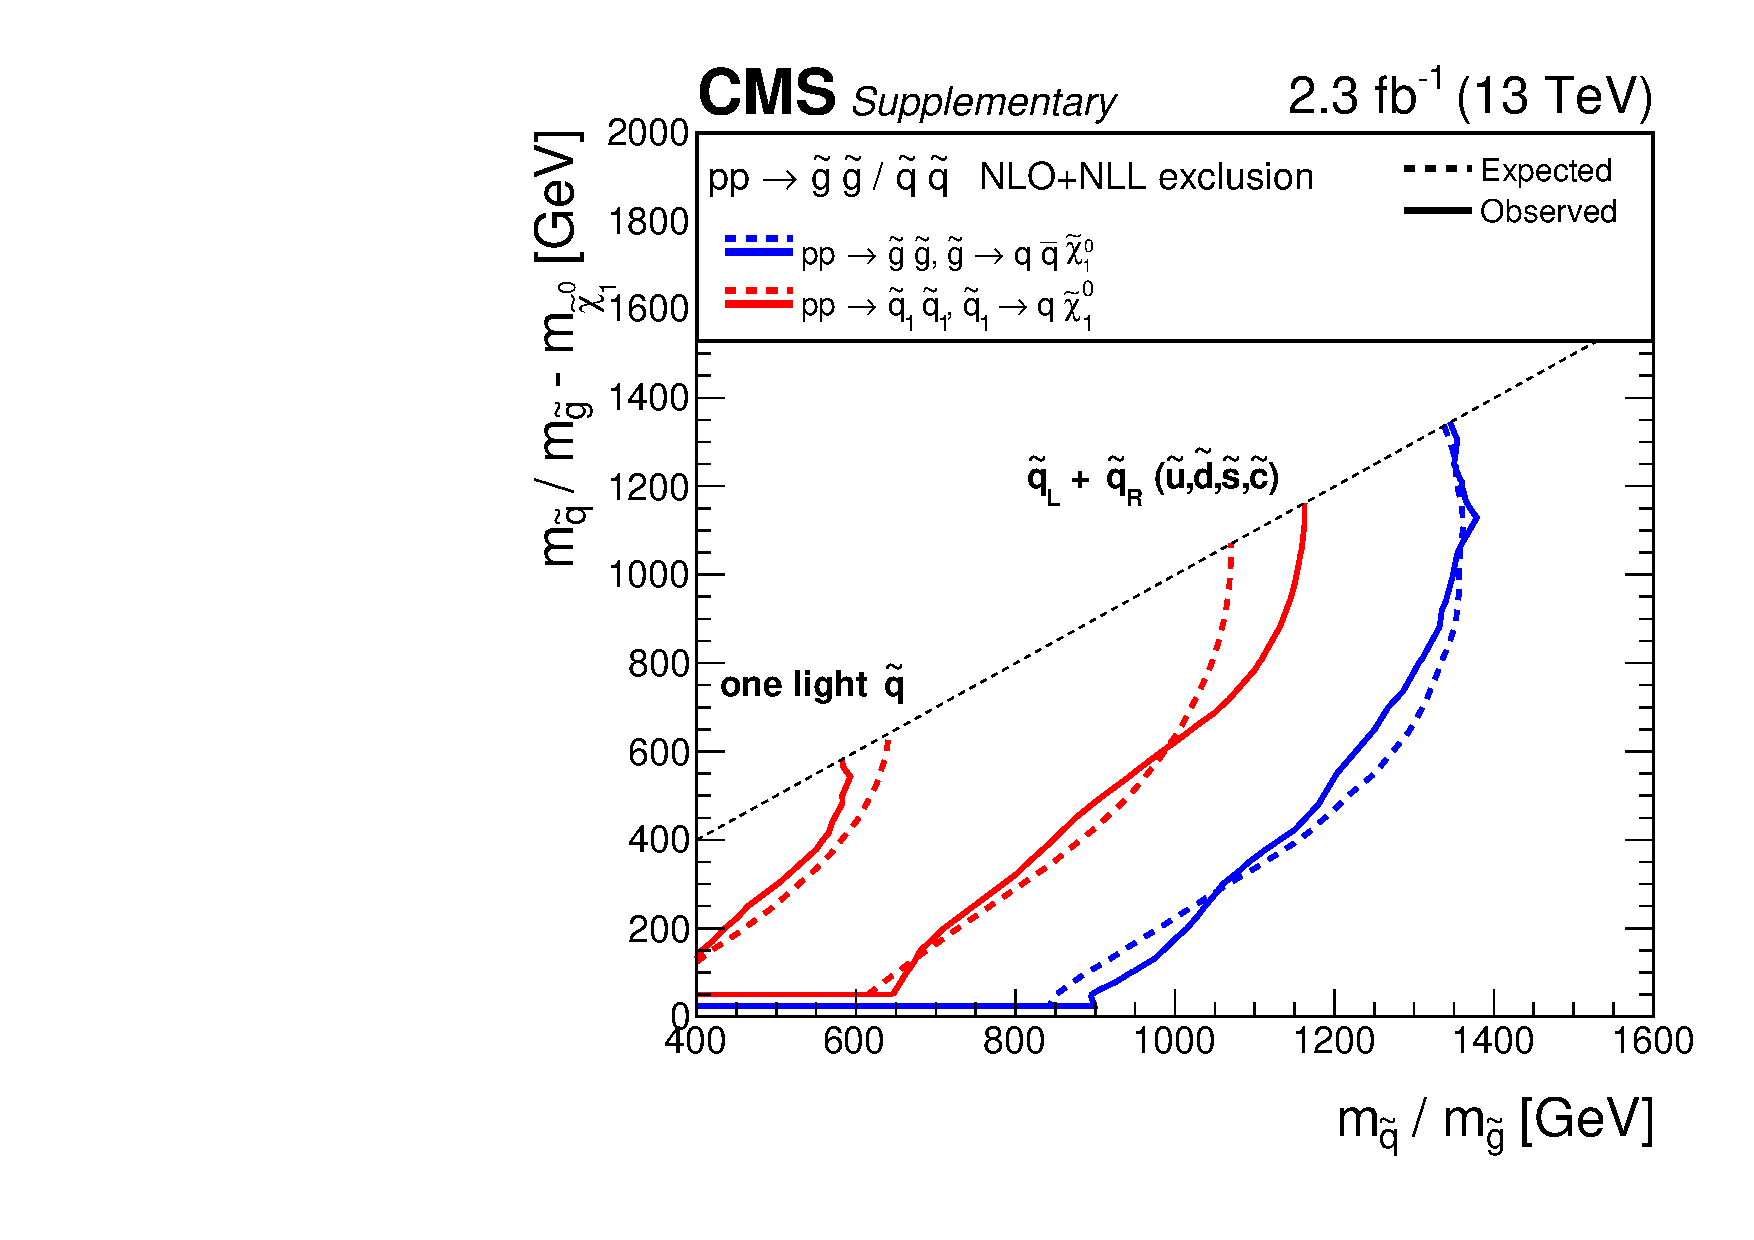
\includegraphics[width=0.49\textwidth]{Supplementary/mixSUMMARY_transposed_aux}
    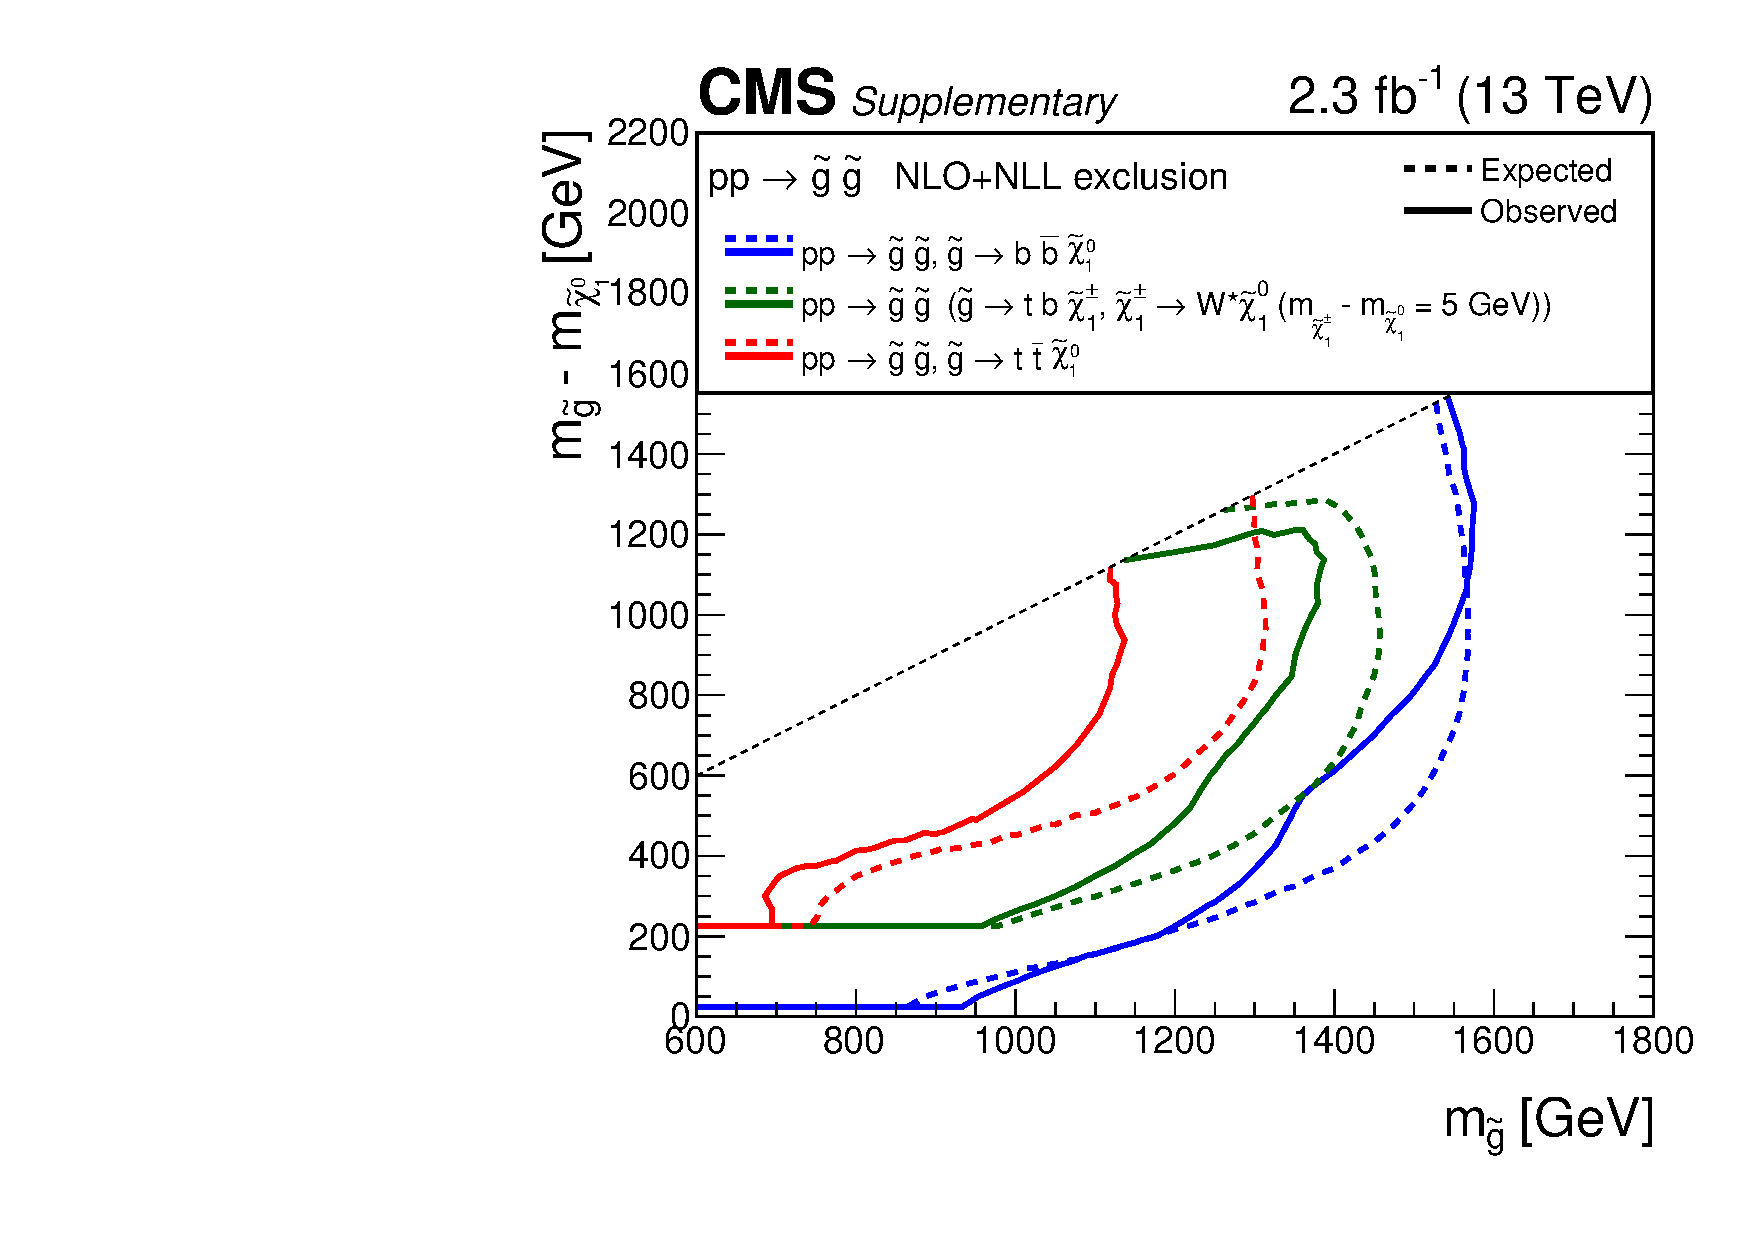
\includegraphics[width=0.49\textwidth]{Supplementary/gluinoSUMMARY_transposed_aux} \\
    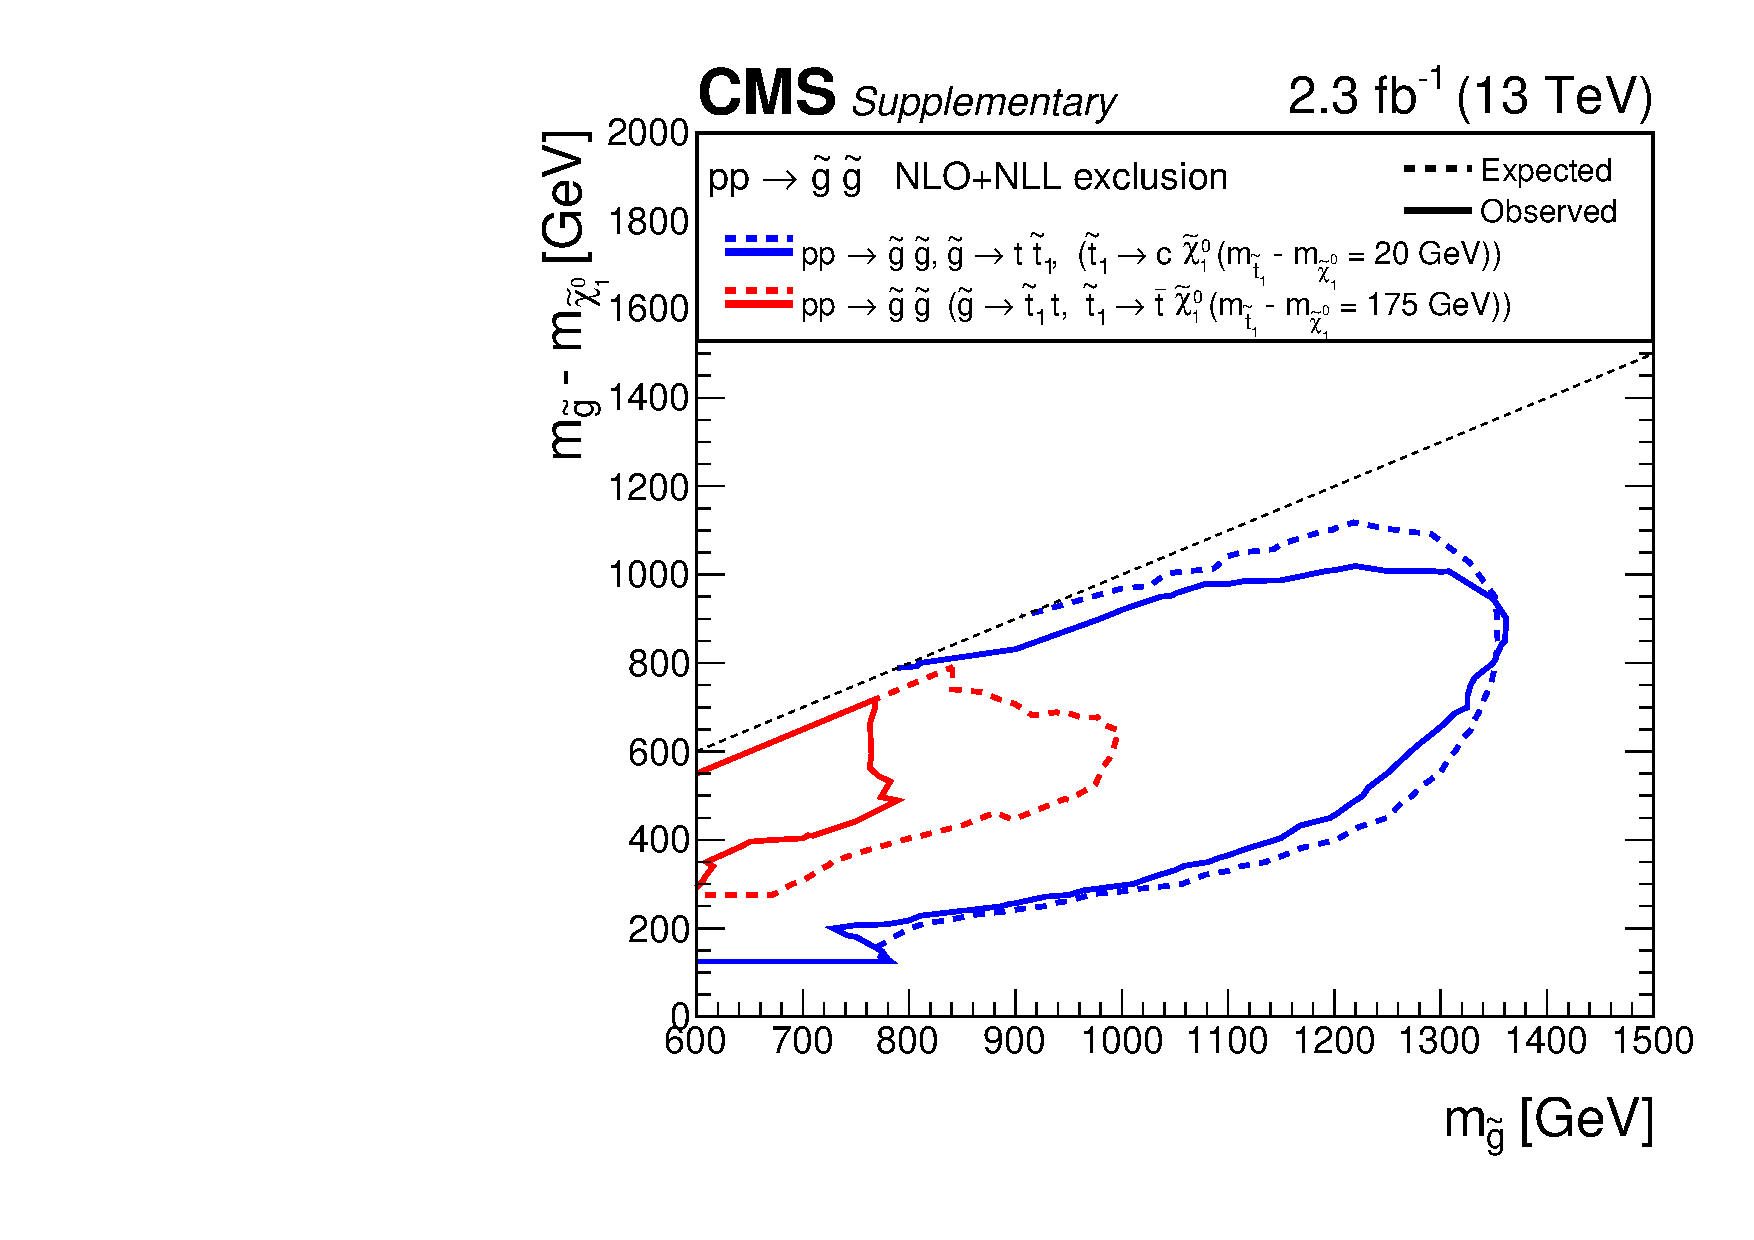
\includegraphics[width=0.49\textwidth]{Supplementary/naturalSUMMARY_transposed_aux}
    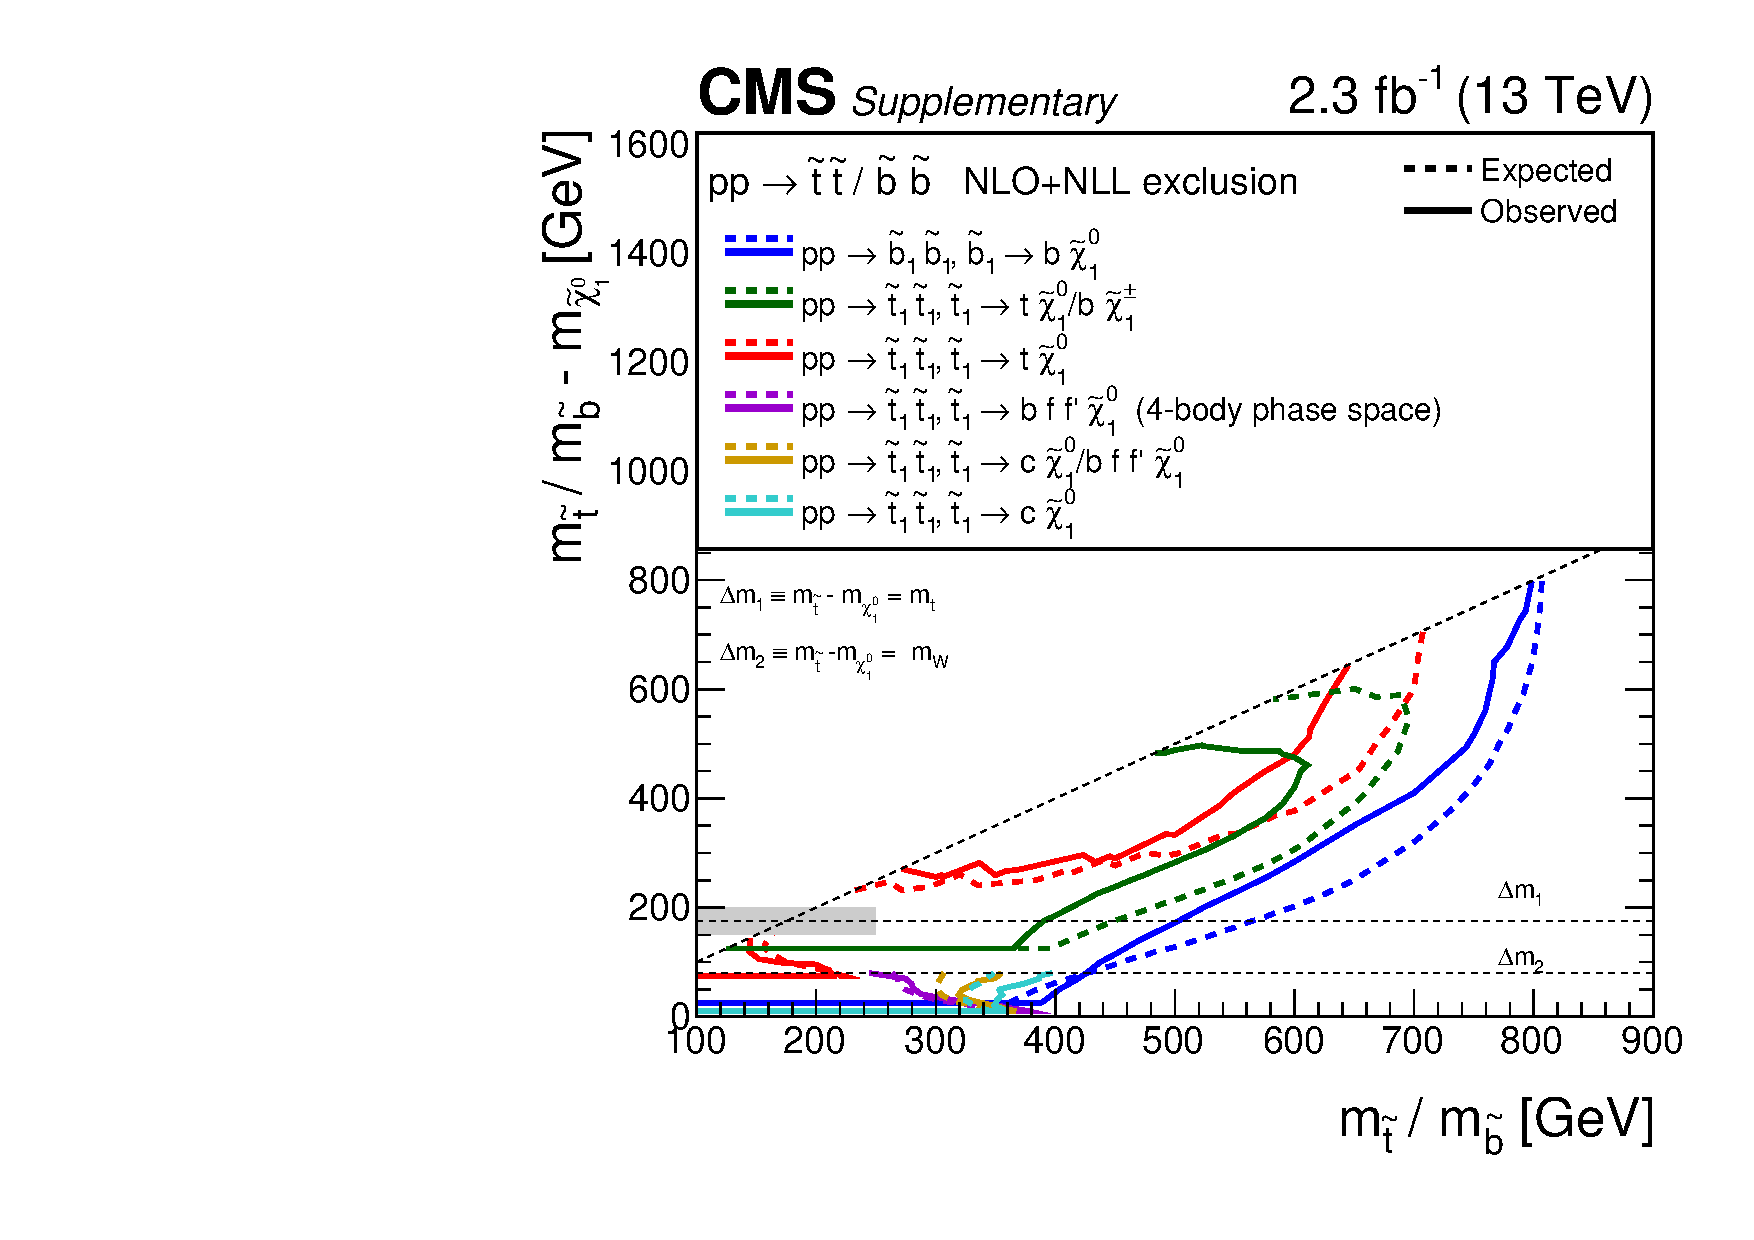
\includegraphics[width=0.49\textwidth]{Supplementary/allThirdGenSUMMARY_transposed_aux} \\
    \caption{Summary for the observed (solid lines) and expected
      (dashed lines) exclusions in the 
      $(m_{\mathrm{SUSY}}, m_{\mathrm{SUSY}} - m_{\PSGczDo})$ plane for
      the models considered in the analysis. Exclusion contours are
      grouped into four summary figures: 
       ``direct and gluino-mediated production of off-shell
       (decoupled) light-flavour squarks'' (top left), 
       ``gluino-mediated production of off-shell (decoupled)
       third-generation squarks'' (top right), ``gluino-mediated
       production of on-shell top squarks'' \ie ``natural'' models
       (bottom left), and ``direct production of third-generation 
       squarks'' (bottom right). 
       \label{fig:summary-excl-plots} }
  \end{center}
\end{figure*}


\clearpage
\begin{figure*}[!h]
  \begin{center}
    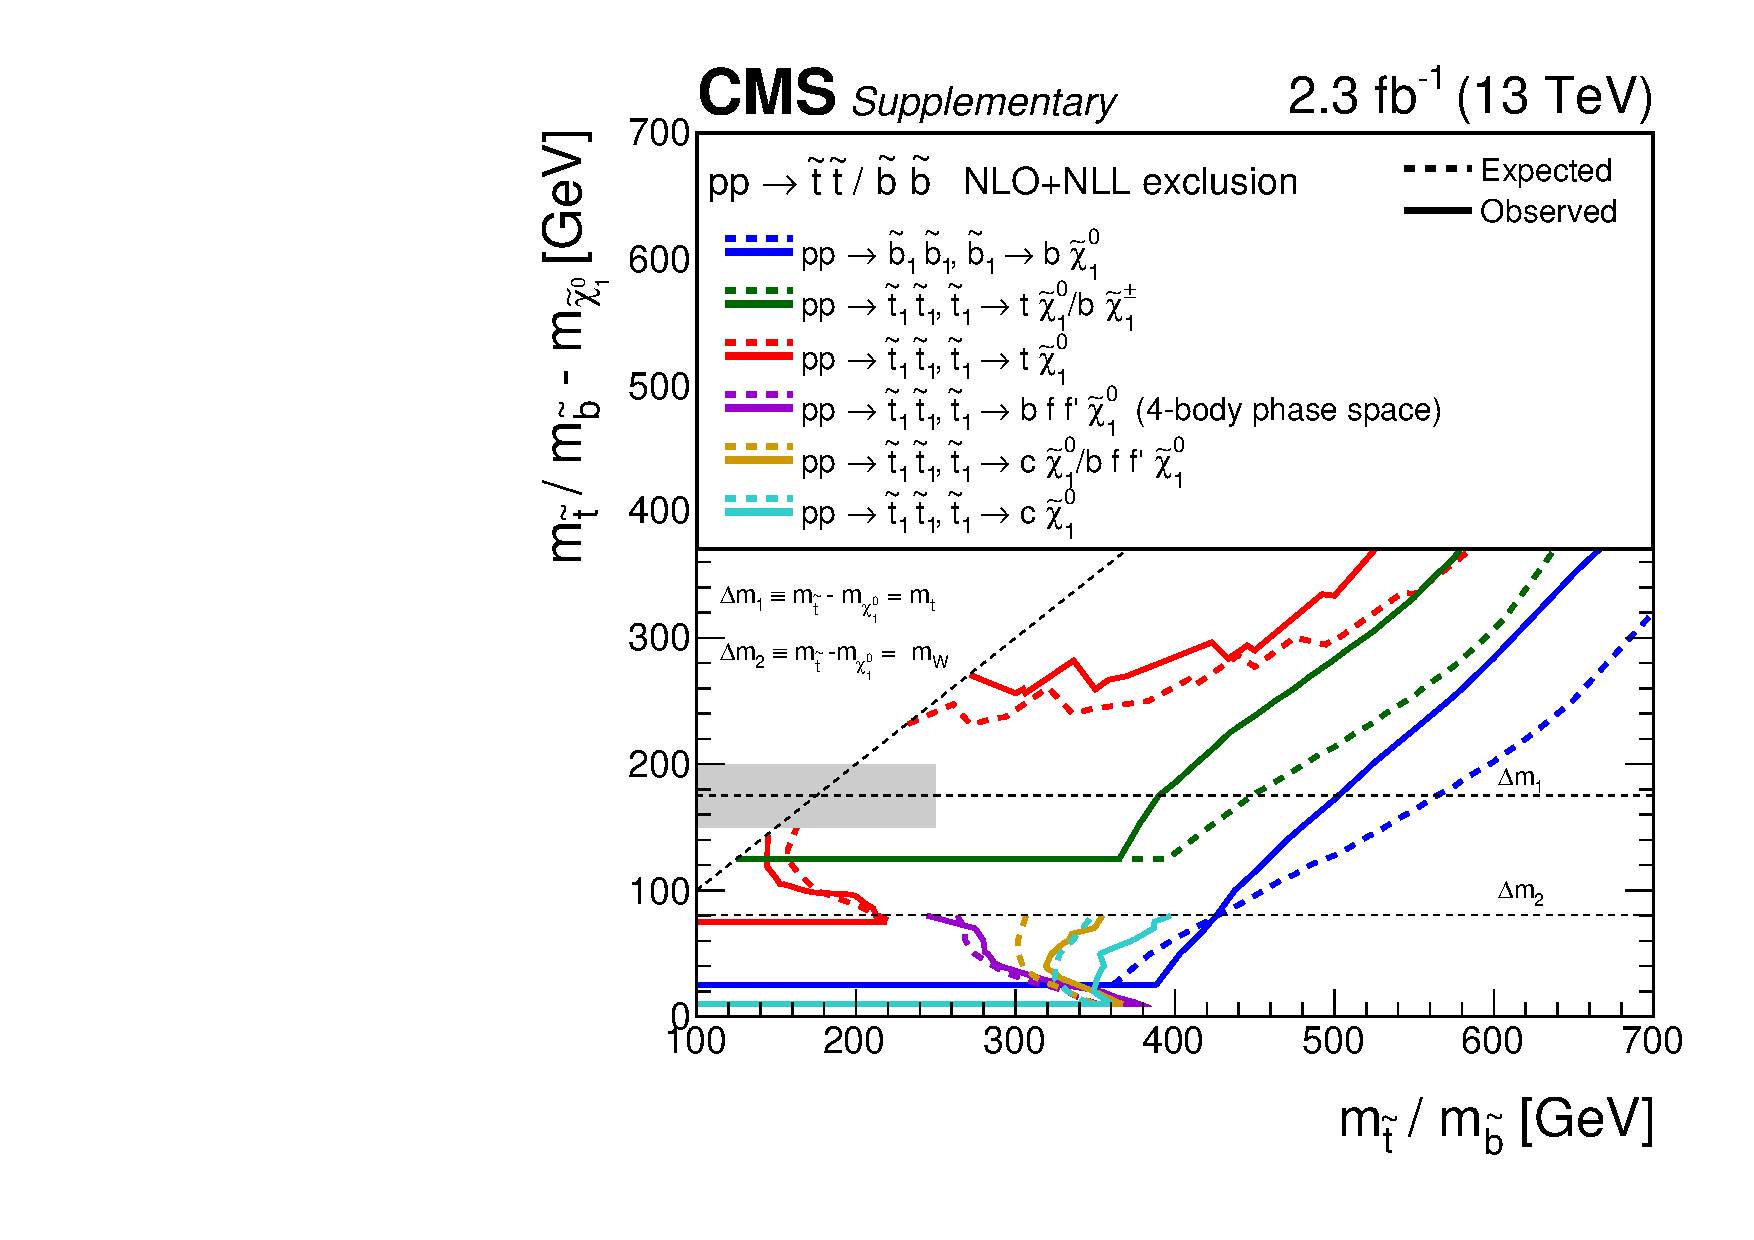
\includegraphics[width=0.49\textwidth]{Supplementary/allThirdGenZoomSUMMARY_transposed_aux} \\
    \caption{Summary for the observed (solid lines) and expected
      (dashed lines) exclusions in the $(m_{\mathrm{SUSY}},
      m_{\mathrm{SUSY}} - m_{\PSGczDo})$ plane for the models
      involving the direct production of third-generation squarks. 
      \label{fig:third-gen-summary-zoomed-plots} }
  \end{center}
\end{figure*}

\clearpage
\section{Material for recasters}

\begin{table*}[h!]
  \centering
  \caption{Summary of a simplified binning scheme comprising \HTmiss
    shapes for eight representative event topologies, defined in terms
    of requirements on \njet (both symmetric and asymmetric
    categories) and \nb. 
    For each topology, event yields are integrated over the full 
    \scalht range, $\scalht > 200\GeV$, and are categorised according
    to eight bins in \HTmiss: $130 < \HTmiss < 200\GeV$, six bins
    100\GeV wide in the region $200 < \HTmiss < 800\GeV$, and an open
    final bin, $\HTmiss > 800\GeV$. 
    This categorisation scheme leads to 64 bins that are exclusive,
    contiguous, and provide complete coverage of the signal region. 
    The corresponding SM background estimates for these 64 bins are
    obtained using the nominal likelihood model. The \HTmiss template 
    for each topology is determined from simulation and the
    normalisation for each template is given by an aggregate of
    estimates from several (\njet, \nb, \scalht) bins, defined
    according to the nominal binning scheme.
    \label{tab:aggr_signal_regions}
  }
  \begin{tabular}{lcccccc}
    \hline
    Topology               & \multicolumn{3}{c}{Aggregate over \dots} &             & \multicolumn{2}{c}{Number of bins in \dots} \\[0.5ex]
    \cline{2-4}
    \cline{6-7}
                           & \njet symm.                              & \njet asym. & \nb     &  & \scalht & \HTmiss              \\[0.5ex]
    \hline
    monojet-like, low \nb  & 1--2                                     & 2           & 0       &  & 1       & 8                    \\
    monojet-like, high \nb & 1--2                                     & 2           & $\geq$1 &  & 1       & 8                    \\
    asymmetric, low \nb    & -                                        & $\geq$3     & 0--1    &  & 1       & 8                    \\
    asymmetric, high \nb   & -                                        & $\geq$3     & $\geq$2 &  & 1       & 8                    \\
    low \njet, low \nb     & 3--4                                     & -           & 0--1    &  & 1       & 8                    \\
    low \njet, high \nb    & 3--4                                     & -           & $\geq$2 &  & 1       & 8                    \\
    high \njet, low \nb    & $\geq$5                                  & -           & 0--1    &  & 1       & 8                    \\
    high \njet, high \nb   & $\geq5$                                  & -           & $\geq$2 &  & 1       & 8                    \\[0.5ex]
    \hline
    Total number of bins   & \multicolumn{5}{c}{}                     & 64                                                        \\[0.5ex]
    \hline
  \end{tabular}
\end{table*}

\clearpage
\begin{table*}[h!]
  \scriptsize
  \centering
  \caption{
    Observed data yields and ``CR-only fit'' SM background
    expectations using the simplified binning scheme, as a function of
    topology and \HTmiss. The SM backgrounds are determined from a 
    simultaneous fit to data in the control regions. The data yields
    in the signal region are masked and excluded from the fit. The
    uncertainties include statistical as well as systematic
    contributions. 
  }
  \label{tab:aggregated}  
  \scalebox{0.85}{
    \begin{tabular}{lllccccccccc}
      \hline
      & \multicolumn{2}{c}{Topology} &      & \multicolumn{8}{c}{\HTmiss bins [GeV]}                                                                                                                      \\[0.5ex]
     \cline{2-3}\cline{5-12}
      & \njet                        & \nb  &  & 130--200           & 200--300             & 300--400           & 400--500         & 500--600         & 600--700        & 700--800       & 800--$\infty$  \\[0.5ex]
      \hline
Data  & mono.                        & low  &  & 2830               & 25115                & 3474               & 745              & 182              & 64              & 22             & 24             \\
SM    & mono.                        & low  &  & $2740 \pm 270$     & $24600.0 \pm 1600$   & $3310 \pm 240$     & $706 \pm 53$     & $208 \pm 39$     & $62 \pm 15$     & $23.9 \pm 5.6$ & $27.6 \pm 5.8$ \\[0.5ex]
Data  & mono.                        & high &  & 320                & 1406                 & 205                & 50               & 12               & 0               & 1              & 0              \\
SM    & mono.                        & high &  & $278 \pm 40$       & $1410 \pm 160$       & $200 \pm 27$       & $45.8 \pm 7.3$   & $12.5 \pm 2.9$   & $3.5 \pm 0.8$   & $1.9 \pm 0.6$  & $1.4 \pm 0.7$  \\[0.5ex]
Data  & asym.                        & low  &  & 3124               & 3367                 & 422                & 75               & 14               & 3               & 3              & 2              \\
SM    & asym.                        & low  &  & $2960 \pm 220$     & $3330 \pm 260$       & $459 \pm 43$       & $78.4 \pm 9.5$   & $15.4 \pm 3.7$   & $4.6 \pm 1.2$   & $3.3 \pm 0.9$  & $3.9 \pm 1.3$  \\[0.5ex]
Data  & asym.                        & high &  & 190                & 133                  & 16                 & 1                & 0                & 0               & 0              & 0              \\
SM    & asym.                        & high &  & $201 \pm 28$       & $138 \pm 26$         & $12.3 \pm 3.0$     & $1.7 \pm 0.5$    & $0.4 \pm 0.2$    & $<0.1$          & $<0.1$         & $0.1 \pm 0.1$  \\[0.5ex]
Data  & low                          & low  &  & 955                & 2027                 & 768                & 228              & 91               & 34              & 15             & 9              \\
SM    & low                          & low  &  & $925 \pm 88$       & $1970 \pm 160$       & $786 \pm 62$       & $251 \pm 23$     & $86 \pm 11$      & $34.7 \pm 4.9$  & $15.4 \pm 1.7$ & $16.5 \pm 2.3$ \\[0.5ex]
Data  & low                          & high &  & 55                 & 77                   & 23                 & 5                & 2                & 1               & 0              & 1              \\
SM    & low                          & high &  & $55 \pm 13$        & $87 \pm 17$          & $21.8 \pm 5.4$     & $5.1 \pm 1.2$    & $1.4 \pm 0.4$    & $0.6 \pm 0.2$   & $0.3 \pm 0.2$  & $0.5 \pm 0.3$  \\[0.5ex]
Data  & high                         & low  &  & 138                & 252                  & 88                 & 36               & 22               & 6               & 3              & 2              \\
SM    & high                         & low  &  & $129 \pm 23$       & $259 \pm 33$         & $111 \pm 13$       & $37.8 \pm 4.2$   & $15.1 \pm 1.8$   & $6.9 \pm 1.1$   & $3.2 \pm 0.6$  & $3.7 \pm 0.8$  \\[0.5ex]
Data  & high                         & high &  & 23                 & 33                   & 14                 & 7                & 0                & 0               & 0              & 0              \\
SM    & high                         & high &  & $22.5 \pm 6.9$     & $32.8 \pm 7.8$       & $10.6 \pm 3.2$     & $2.5 \pm 0.9$    & $0.9 \pm 0.3$    & $0.4 \pm 0.2$   & $0.4 \pm 0.1$  & $0.1 \pm 0.1$  \\[0.5ex]
%Data & mono.                        & low  &  & 2830               & 25115                & 3474               & 745              & 182              & 64              & 22             & 24             \\
%SM   & mono.                        & low  &  & $2740.0 \pm 268.0$ & $24600.0 \pm 1600.0$ & $3310.0 \pm 242.0$ & $706.0 \pm 52.9$ & $208.0 \pm 38.5$ & $61.8 \pm 15.1$ & $23.9 \pm 5.6$ & $27.6 \pm 5.8$ \\[0.5ex]
%Data & mono.                        & high &  & 320                & 1406                 & 205                & 50               & 12               & 0               & 1              & 0              \\
%SM   & mono.                        & high &  & $278.0 \pm 39.5$   & $1410.0 \pm 162.0$   & $200.0 \pm 27.1$   & $45.8 \pm 7.3$   & $12.5 \pm 2.9$   & $3.5 \pm 0.8$   & $1.9 \pm 0.6$  & $1.4 \pm 0.7$  \\[0.5ex]
%Data & asym.                        & low  &  & 3124               & 3367                 & 422                & 75               & 14               & 3               & 3              & 2              \\
%SM   & asym.                        & low  &  & $2960.0 \pm 217.0$ & $3330.0 \pm 258.0$   & $459.0 \pm 42.6$   & $78.4 \pm 9.5$   & $15.4 \pm 3.7$   & $4.6 \pm 1.2$   & $3.3 \pm 0.9$  & $3.9 \pm 1.3$  \\[0.5ex]
%Data & asym.                        & high &  & 190                & 133                  & 16                 & 1                & 0                & 0               & 0              & 0              \\
%SM   & asym.                        & high &  & $201.0 \pm 28.1$   & $138.0 \pm 26.0$     & $12.3 \pm 3.0$     & $1.7 \pm 0.5$    & $0.4 \pm 0.2$    & $0.0 \pm 0.0$   & $0.0 \pm 0.0$  & $0.1 \pm 0.1$  \\[0.5ex]
%Data & low                          & low  &  & 955                & 2027                 & 768                & 228              & 91               & 34              & 15             & 9              \\
%SM   & low                          & low  &  & $925.0 \pm 87.8$   & $1970.0 \pm 157.0$   & $786.0 \pm 62.0$   & $251.0 \pm 22.6$ & $86.2 \pm 10.5$  & $34.7 \pm 4.9$  & $15.4 \pm 1.7$ & $16.5 \pm 2.3$ \\[0.5ex]
%Data & low                          & high &  & 55                 & 77                   & 23                 & 5                & 2                & 1               & 0              & 1              \\
%SM   & low                          & high &  & $55.4 \pm 12.8$    & $87.1 \pm 17.4$      & $21.8 \pm 5.4$     & $5.1 \pm 1.2$    & $1.4 \pm 0.4$    & $0.6 \pm 0.2$   & $0.3 \pm 0.2$  & $0.5 \pm 0.3$  \\[0.5ex]
%Data & high                         & low  &  & 138                & 252                  & 88                 & 36               & 22               & 6               & 3              & 2              \\
%SM   & high                         & low  &  & $129.0 \pm 22.5$   & $259.0 \pm 32.7$     & $111.0 \pm 12.6$   & $37.8 \pm 4.2$   & $15.1 \pm 1.8$   & $6.9 \pm 1.1$   & $3.2 \pm 0.6$  & $3.7 \pm 0.8$  \\[0.5ex]
%Data & high                         & high &  & 23                 & 33                   & 14                 & 7                & 0                & 0               & 0              & 0              \\
%SM   & high                         & high &  & $22.5 \pm 6.9$     & $32.8 \pm 7.8$       & $10.6 \pm 3.2$     & $2.5 \pm 0.9$    & $0.9 \pm 0.3$    & $0.4 \pm 0.2$   & $0.4 \pm 0.1$  & $0.1 \pm 0.0$  \\[0.5ex]
      \hline
    \end{tabular}
  }
\end{table*}

\newcommand{\customcaption}[4]{(Upper panel) Event yields observed in
  data (solid circles) and SM expectations with their associated
  uncertainties (blue histogram with grey shaded band) determined from
  a simultaneous fit to data in the control regions only (CR-only
  fit). Event yields and expectations are shown as a function of
  \HTmiss for events in the #1 topology that are required to satisfy
  #2, $\scalht > 200\GeV$, and (\cmsLeft) #3 or (\cmsRight) #4.
  (Lower panel) The significance of deviations (pulls) observed in
  data with respect to both the SM expectations from the CR-only fit,
  expressed in terms of the total uncertainty in the SM
  expectations. The pulls cannot be considered independently due to
  inter-bin correlations.}

%\newcommand{\customcaption}[4]{(Upper panel) Event yields observed in
%  data (solid circles) and SM expectations with their associated
%  uncertainties (blue histogram with grey shaded band) determined from
%  a simultaneous fit to data in the control regions only (CR-only
%  fit), as a function of \HTmiss for events in the #1 topology that
%  satisfy $\scalht > 200\GeV$, #2, and (\cmsLeft) #3 or (\cmsRight)
%  #4.  (Lower panel) The significance of deviations (pulls) observed
%  in data with respect to both the SM expectations from the CR-only
%  fit, expressed in terms of the total uncertainty in the SM
%  expectations. The pulls cannot be considered independently due to
%  inter-bin correlations.}

\clearpage
\begin{figure*}[!h]
  \begin{center}
    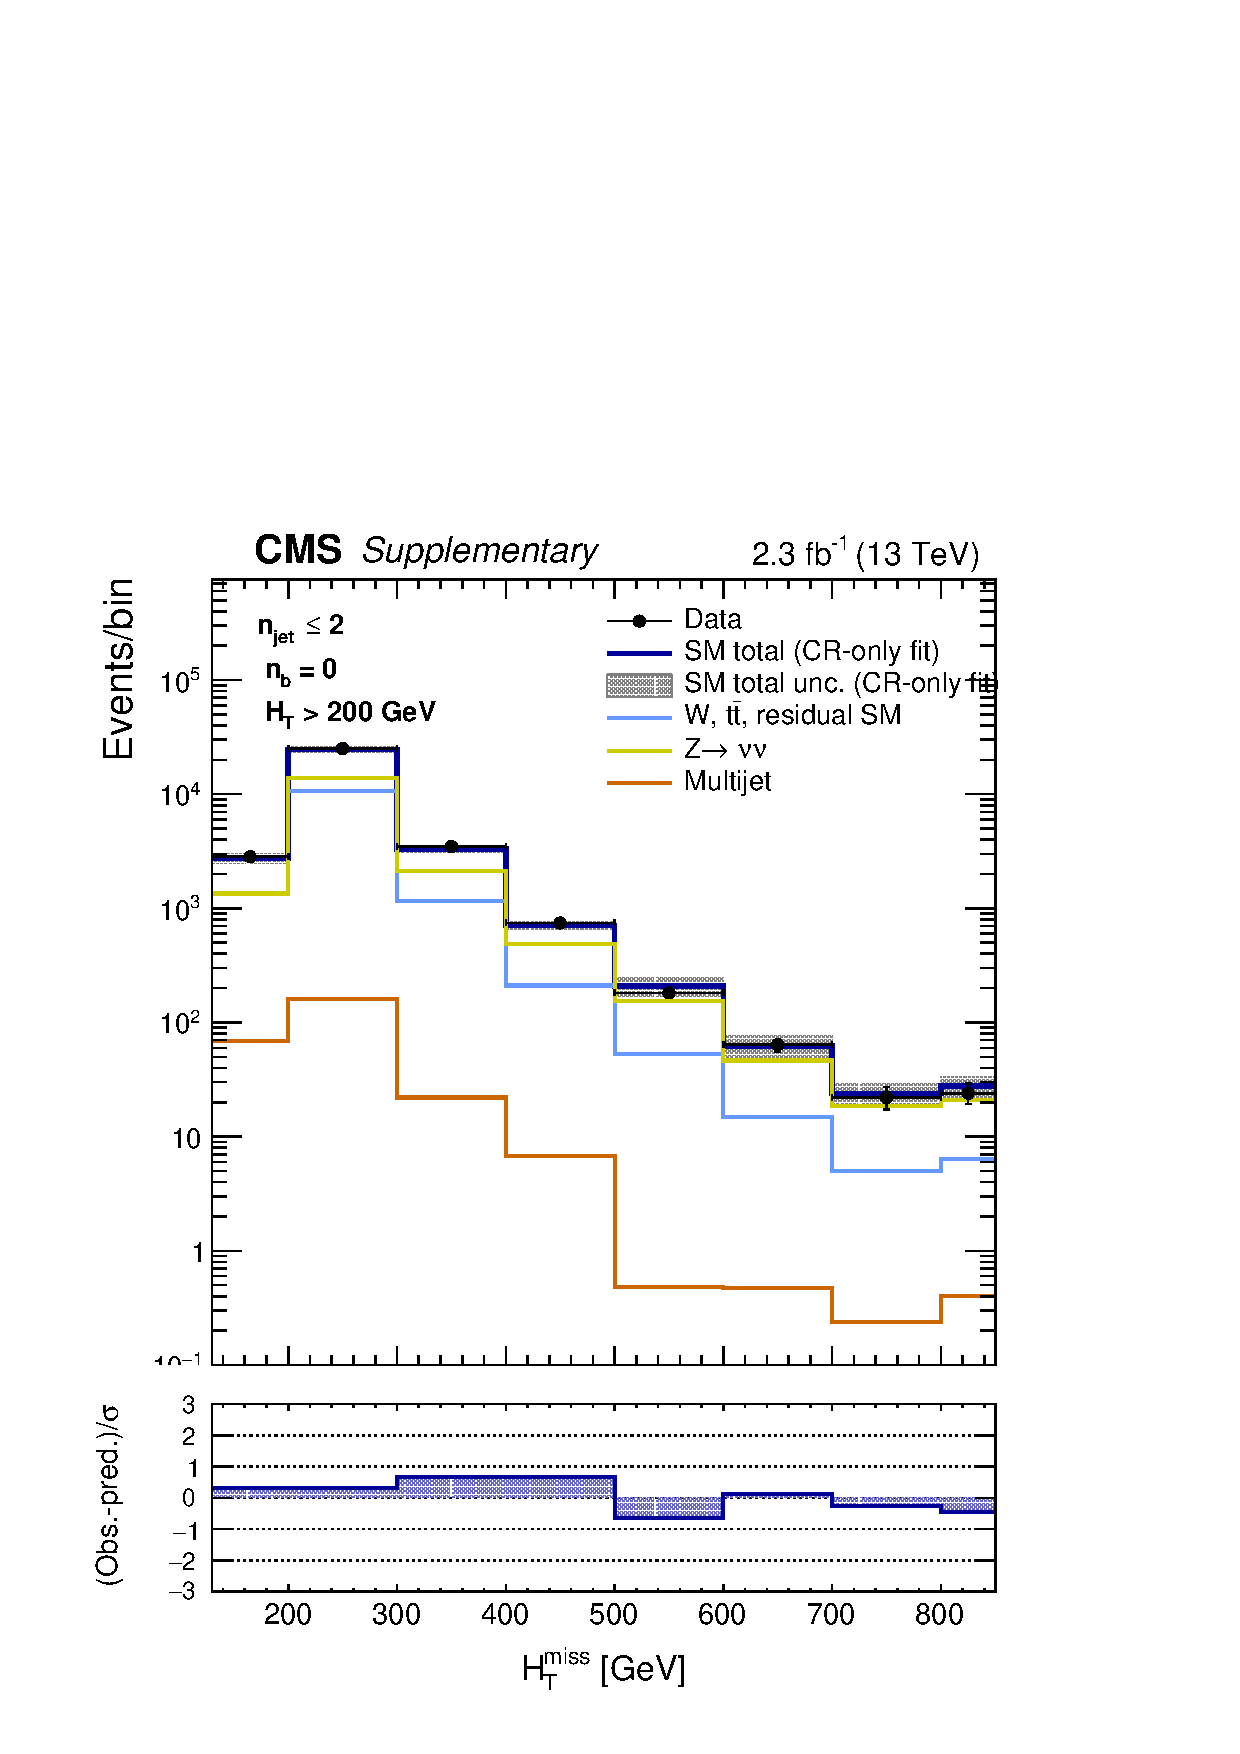
\includegraphics[width=0.49\textwidth]{Supplementary/aggregated_mhtShape_eq0b_le2j_200_Inf_crfit_aux.pdf} 
    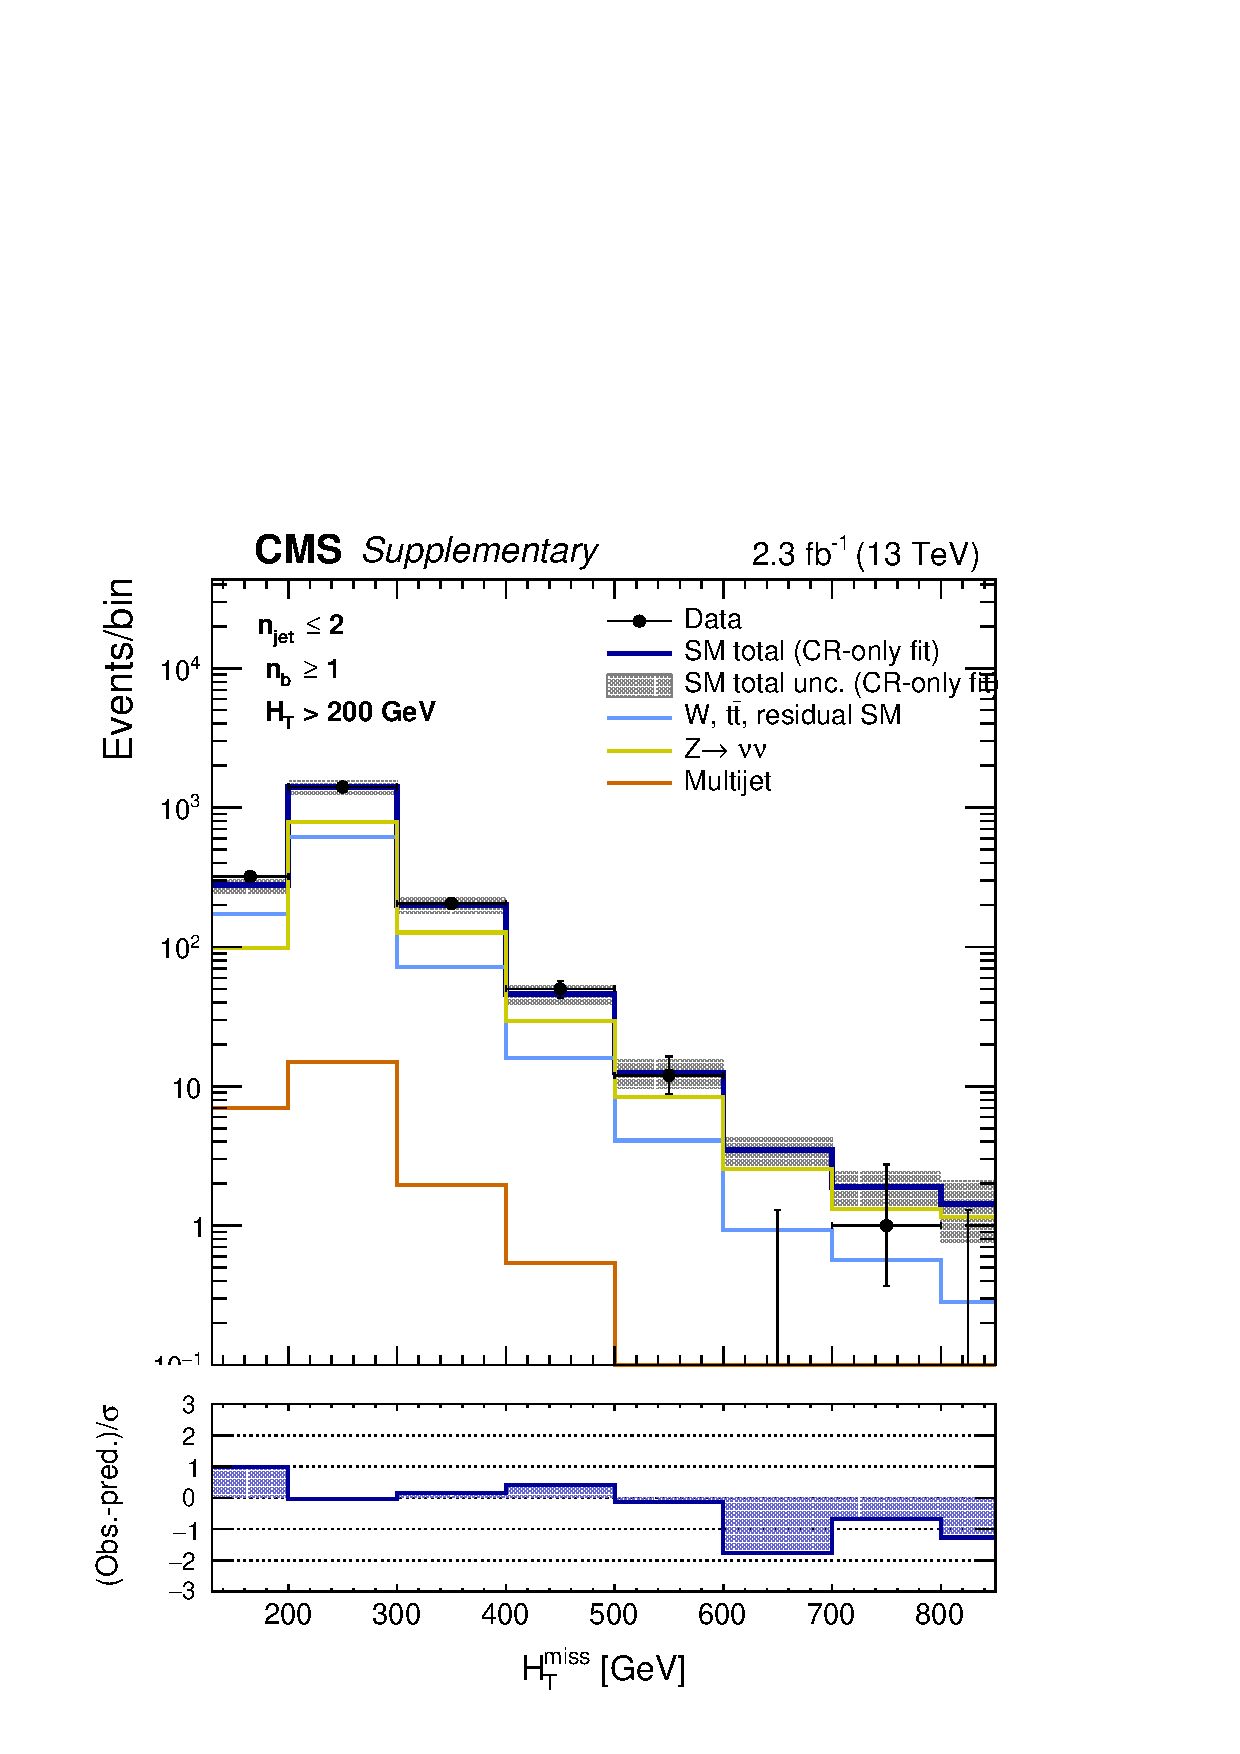
\includegraphics[width=0.49\textwidth]{Supplementary/aggregated_mhtShape_ge1b_le2j_200_Inf_crfit_aux.pdf} \\
    \caption{\customcaption{``monojet-like''}{$1 \leq \njet \leq 2$ or $\njetasym = 2$}{$\nb = 0$}{$\nb \geq 1$}
      \label{fig:aggr_monojet} 
    }
  \end{center}
\end{figure*}

\clearpage
\begin{figure*}[!h]
  \begin{center}
    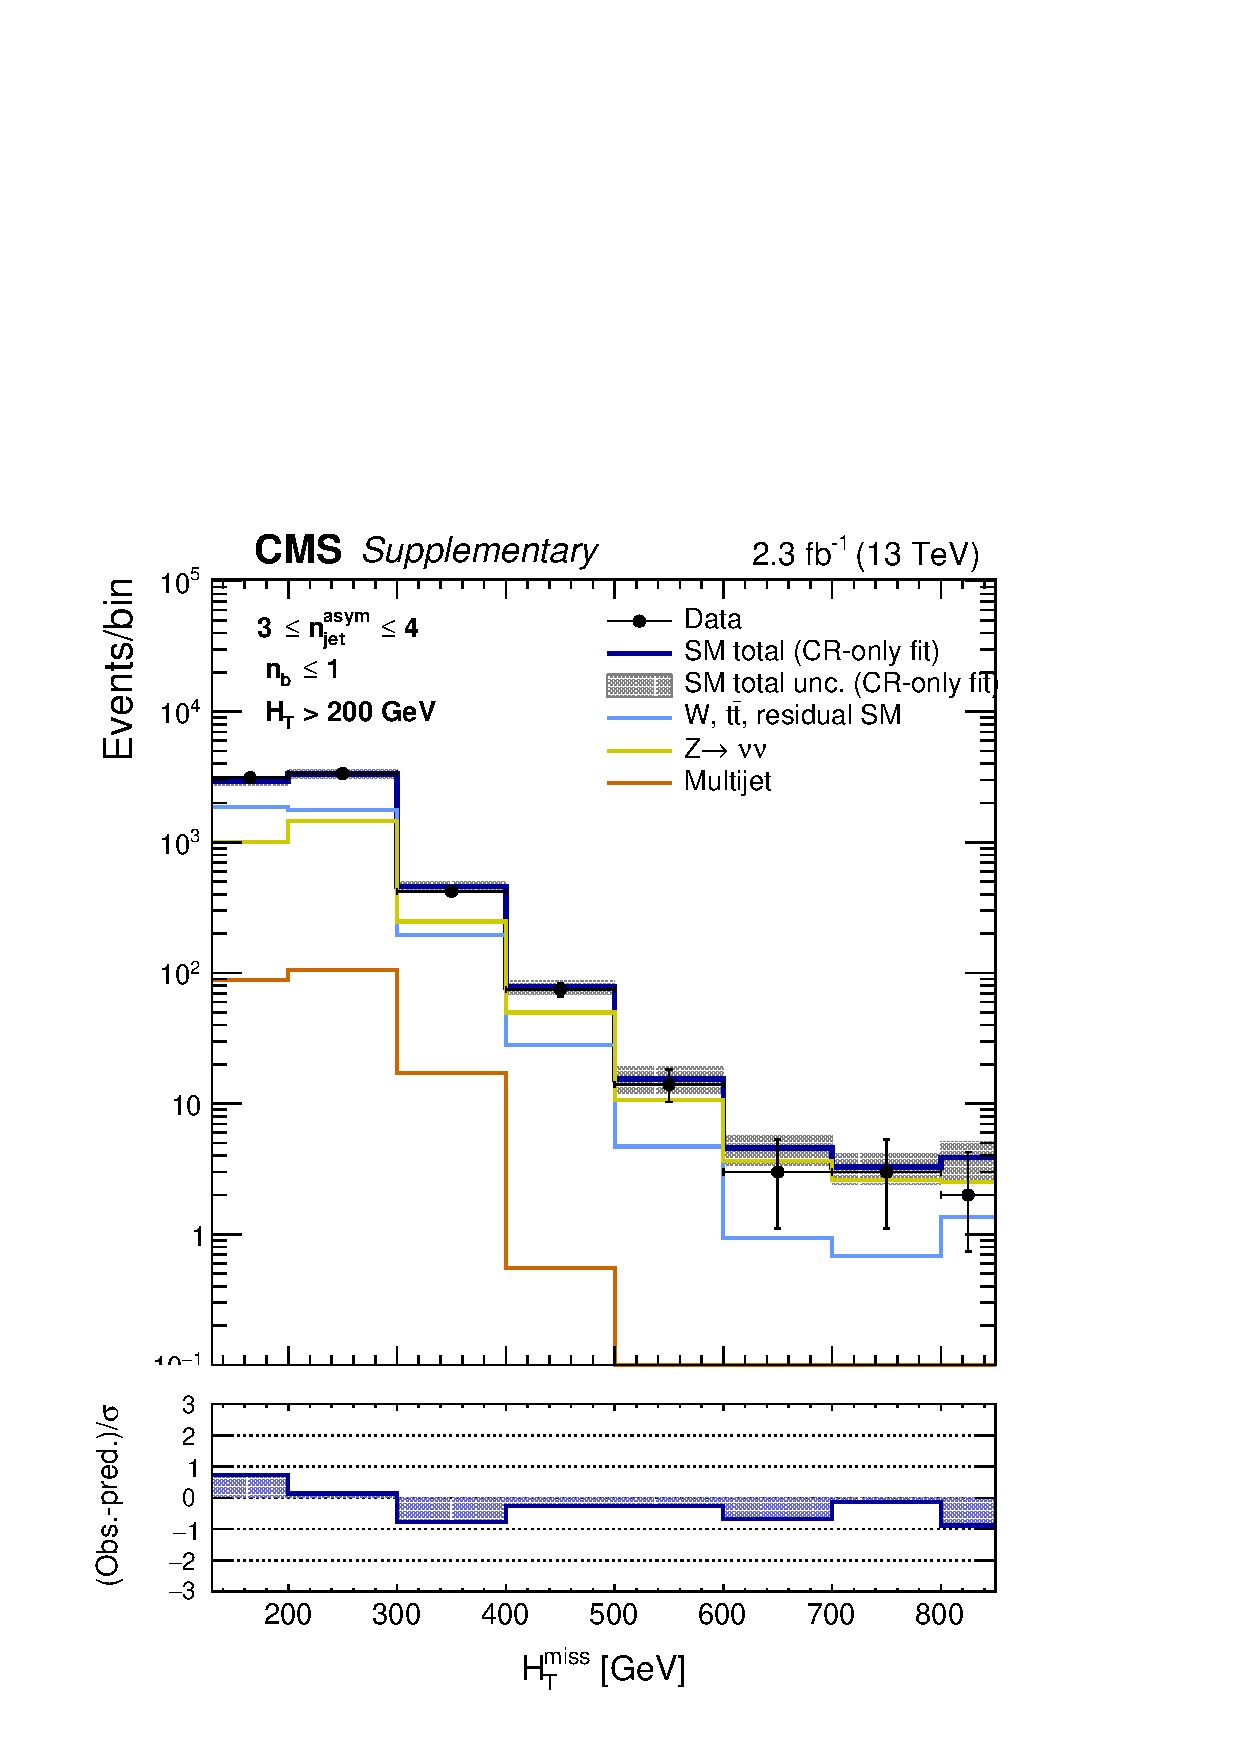
\includegraphics[width=0.49\textwidth]{Supplementary/aggregated_mhtShape_le1b_ge3a_200_Inf_crfit_aux.pdf} 
    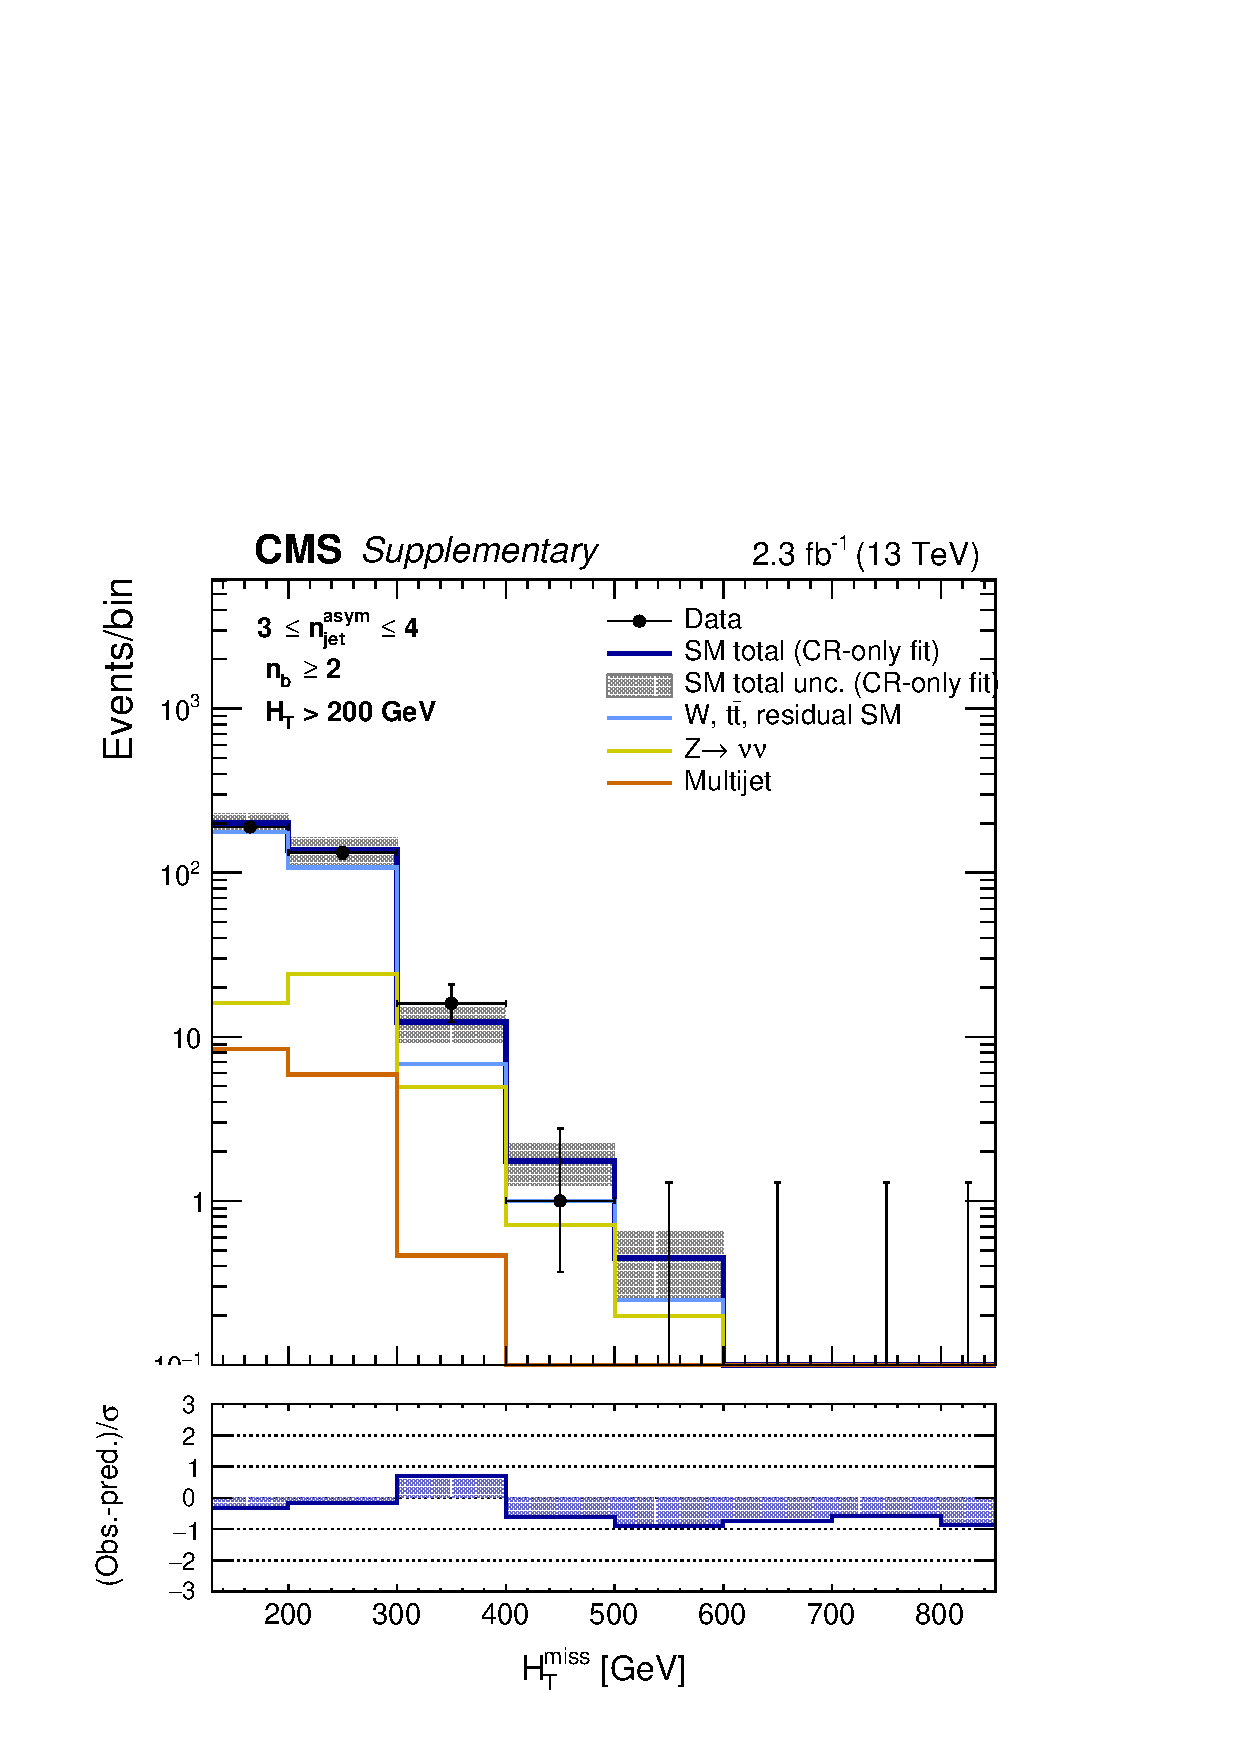
\includegraphics[width=0.49\textwidth]{Supplementary/aggregated_mhtShape_ge2b_ge3a_200_Inf_crfit_aux.pdf} \\
    \caption{\customcaption{``asymmetric''}{$\njetasym \geq 3$}{$0 \leq \nb \leq 1$}{$\nb \geq 2$}
      \label{fig:aggr_asym} 
    }
  \end{center}
\end{figure*}

\clearpage
\begin{figure*}[!h]
  \begin{center}
    \includegraphics[width=0.49\textwidth]{Supplementary/aggregated_mhtShape_le1b_ge3j_200_Inf_crfit_aux.pdf} 
    \includegraphics[width=0.49\textwidth]{Supplementary/aggregated_mhtShape_ge2b_ge3j_200_Inf_crfit_aux.pdf} \\
    \caption{\customcaption{``low \njet''}{$3 \leq \njet \leq 4$}{$0 \leq \nb \leq 1$}{$\nb \geq 2$}
      \label{fig:aggr_mid} 
    }
  \end{center}
\end{figure*}

\clearpage
\begin{figure*}[!h]
  \begin{center}
    \includegraphics[width=0.49\textwidth]{Supplementary/aggregated_mhtShape_le1b_ge5j_200_Inf_crfit_aux.pdf} 
    \includegraphics[width=0.49\textwidth]{Supplementary/aggregated_mhtShape_ge2b_ge5j_200_Inf_crfit_aux.pdf} \\
    \caption{\customcaption{``high \njet''}{$\njet \geq 5$}{$0 \leq \nb \leq 1$}{$\nb \geq 2$}
      \label{fig:aggr_high} 
    }
  \end{center}
\end{figure*}

\clearpage
\begin{figure*}[!h]
  \begin{center}
    \includegraphics[width=\textwidth]{Supplementary/aggregated_covariance_aux.pdf} 
    \caption{Covariance matrix for the SM background estimates
      obtained using the simplified binning scheme, determined from a
      simultaneous fit to data in the control regions only (CR-only
      fit). The uncertainties in the background estimates are
      correlated in such a way that the covariance is typically
      positive. Small positive values, as well as the few negative
      values, are not shown.  
      \label{fig:aggr_corr} 
    }
  \end{center}
\end{figure*}

\clearpage
\begin{figure*}[!h]
  \begin{center}
    \includegraphics[width=\textwidth]{Supplementary/aggregated_correlation_aux.pdf} 
    \caption{Correlation matrix for the SM background estimates
      obtained using the simplified binning scheme, determined from a
      simultaneous fit to data in the control regions only (CR-only
      fit).  
      \label{fig:aggr_corr} 
    }
  \end{center}
\end{figure*}

\clearpage
\begin{table*}[!t]
  \topcaption{Expected ($\mu_{\text{exp}}$) and observed 
    ($\mu_{\text{obs}}$) upper limits on the production cross section, 
    expressed in terms of the signal strength parameter, obtained using
    both the nominal and simplified binning schema. Comparable values
    are obtained from the two schema for these benchmark SUSY models
    because the signal events typically populate bins at high values
    of \scalht and \HTmiss and so are at or near the limit of the
    search sensitivity. Larger differences in $\mu$ can be observed
    for models that populate the core of these distributions. 
  }
  \label{tab:aggr_limits}
  \centering
  \begin{tabular}{ llccccc }
    \hline
    \multicolumn{2}{c}{Benchmark models}    & \multicolumn{2}{c}{Nominal}
                                            & 
                                            & \multicolumn{2}{c}{Simplified}             \\ [0.3ex]
    \cline{3-4}
    \cline{6-7}
    \multicolumn{2}{c}{$(m_{\text{SUSY}}, m_{\mathrm{LSP}})$ [\GeVns{}]} 
                                            & $\mu_{\text{exp}}$
                                            & $\mu_{\text{obs}}$
                                            & 
                                            & $\mu_{\text{exp}}$
                                            & $\mu_{\text{obs}}$                         \\ [0.3ex]
    \hline
    \multirow{2}{*}{\texttt{T1qqqq}}        & (1300, 100) & 0.79 & 0.76 &  & 0.89 & 0.65 \\
                                            & (900, 700)  & 0.58 & 0.44 &  & 0.72 & 0.54 \\ [0.5ex]
    \multirow{2}{*}{\texttt{T2qq\_8fold}}   & (1050, 100) & 0.90 & 0.63 &  & 1.05 & 0.56 \\
                                            & (650, 550)  & 0.93 & 0.80 &  & 1.23 & 0.86 \\ [0.5ex]
    \multirow{2}{*}{\texttt{T2qq\_1fold}}   & (600, 50)   & 0.78 & 0.84 &  & 1.20 & 1.23 \\
                                            & (400, 250)  & 0.73 & 0.71 &  & 1.04 & 0.84 \\ [0.5ex]
    \multirow{2}{*}{\texttt{T1bbbb}}        & (1500, 100) & 0.81 & 0.79 &  & 1.04 & 0.83 \\
                                            & (1000, 800) & 0.33 & 0.32 &  & 0.57 & 0.90 \\ [0.5ex]
    \multirow{2}{*}{\texttt{T1tttt}}        & (1300, 100) & 1.00 & 1.89 &  & 1.41 & 1.20 \\
                                            & (800, 400)  & 0.56 & 1.03 &  & 1.32 & 1.92 \\ [0.5ex]
    \multirow{2}{*}{\texttt{T1ttbb}}        & (1300, 100) & 0.60 & 0.91 &  & 0.86 & 0.72 \\
                                            & (1000, 700) & 0.51 & 0.70 &  & 0.89 & 1.51 \\ [0.5ex]
    \multirow{2}{*}{\texttt{T5tttt\_DM175}} & (800, 100)  & 0.69 & 1.19 &  & 0.97 & 1.40 \\
                                            & (700, 400)  & 1.00 & 1.35 &  & 2.01 & 3.21 \\ [0.5ex]
    \multirow{2}{*}{\texttt{T5ttcc}}        & (1200, 200) & 0.58 & 0.87 &  & 0.80 & 0.67 \\
                                            & (750, 600)  & 0.89 & 0.72 &  & 1.36 & 1.08 \\ [0.5ex]
    \multirow{2}{*}{\texttt{T2bb}}          & (800, 50)   & 0.96 & 1.06 &  & 1.60 & 1.09 \\
                                            & (375, 300)  & 0.67 & 0.87 &  & 1.24 & 1.31 \\ [0.5ex]
    \multirow{2}{*}{\texttt{T2tb}}          & (600, 50)   & 0.70 & 1.35 &  & 0.97 & 1.48 \\
                                            & (350, 225)  & 0.79 & 0.88 &  & 1.62 & 1.77 \\ [0.5ex]
    \multirow{2}{*}{\texttt{T2tt}}          & (700, 50)   & 0.90 & 1.19 &  & 1.16 & 1.58 \\
                                            & (350, 100)  & 0.44 & 0.50 &  & 0.82 & 0.96 \\ [0.5ex]
    \multirow{1}{*}{\texttt{T2cc}}          & (325, 305)  & 0.92 & 0.68 &  & 1.31 & 0.95 \\ [0.5ex]
    \multirow{1}{*}{\texttt{T2tt\_degen}}   & (300, 290)  & 0.56 & 0.41 &  & 0.77 & 0.57 \\ [0.5ex]
    \multirow{1}{*}{\texttt{T2tt\_mixed}}   & (300, 250)  & 0.99 & 0.58 &  & 1.41 & 1.08 \\ [0.5ex]
    \hline
  \end{tabular}
\end{table*}

